% Options for packages loaded elsewhere
\PassOptionsToPackage{unicode}{hyperref}
\PassOptionsToPackage{hyphens}{url}
\PassOptionsToPackage{dvipsnames,svgnames,x11names}{xcolor}
%
\documentclass[
  letterpaper,
  DIV=11,
  numbers=noendperiod]{scrreprt}

\usepackage{amsmath,amssymb}
\usepackage{iftex}
\ifPDFTeX
  \usepackage[T1]{fontenc}
  \usepackage[utf8]{inputenc}
  \usepackage{textcomp} % provide euro and other symbols
\else % if luatex or xetex
  \usepackage{unicode-math}
  \defaultfontfeatures{Scale=MatchLowercase}
  \defaultfontfeatures[\rmfamily]{Ligatures=TeX,Scale=1}
\fi
\usepackage{lmodern}
\ifPDFTeX\else  
    % xetex/luatex font selection
\fi
% Use upquote if available, for straight quotes in verbatim environments
\IfFileExists{upquote.sty}{\usepackage{upquote}}{}
\IfFileExists{microtype.sty}{% use microtype if available
  \usepackage[]{microtype}
  \UseMicrotypeSet[protrusion]{basicmath} % disable protrusion for tt fonts
}{}
\makeatletter
\@ifundefined{KOMAClassName}{% if non-KOMA class
  \IfFileExists{parskip.sty}{%
    \usepackage{parskip}
  }{% else
    \setlength{\parindent}{0pt}
    \setlength{\parskip}{6pt plus 2pt minus 1pt}}
}{% if KOMA class
  \KOMAoptions{parskip=half}}
\makeatother
\usepackage{xcolor}
\usepackage{soul}
\setlength{\emergencystretch}{3em} % prevent overfull lines
\setcounter{secnumdepth}{5}
% Make \paragraph and \subparagraph free-standing
\ifx\paragraph\undefined\else
  \let\oldparagraph\paragraph
  \renewcommand{\paragraph}[1]{\oldparagraph{#1}\mbox{}}
\fi
\ifx\subparagraph\undefined\else
  \let\oldsubparagraph\subparagraph
  \renewcommand{\subparagraph}[1]{\oldsubparagraph{#1}\mbox{}}
\fi

\usepackage{color}
\usepackage{fancyvrb}
\newcommand{\VerbBar}{|}
\newcommand{\VERB}{\Verb[commandchars=\\\{\}]}
\DefineVerbatimEnvironment{Highlighting}{Verbatim}{commandchars=\\\{\}}
% Add ',fontsize=\small' for more characters per line
\usepackage{framed}
\definecolor{shadecolor}{RGB}{241,243,245}
\newenvironment{Shaded}{\begin{snugshade}}{\end{snugshade}}
\newcommand{\AlertTok}[1]{\textcolor[rgb]{0.68,0.00,0.00}{#1}}
\newcommand{\AnnotationTok}[1]{\textcolor[rgb]{0.37,0.37,0.37}{#1}}
\newcommand{\AttributeTok}[1]{\textcolor[rgb]{0.40,0.45,0.13}{#1}}
\newcommand{\BaseNTok}[1]{\textcolor[rgb]{0.68,0.00,0.00}{#1}}
\newcommand{\BuiltInTok}[1]{\textcolor[rgb]{0.00,0.23,0.31}{#1}}
\newcommand{\CharTok}[1]{\textcolor[rgb]{0.13,0.47,0.30}{#1}}
\newcommand{\CommentTok}[1]{\textcolor[rgb]{0.37,0.37,0.37}{#1}}
\newcommand{\CommentVarTok}[1]{\textcolor[rgb]{0.37,0.37,0.37}{\textit{#1}}}
\newcommand{\ConstantTok}[1]{\textcolor[rgb]{0.56,0.35,0.01}{#1}}
\newcommand{\ControlFlowTok}[1]{\textcolor[rgb]{0.00,0.23,0.31}{#1}}
\newcommand{\DataTypeTok}[1]{\textcolor[rgb]{0.68,0.00,0.00}{#1}}
\newcommand{\DecValTok}[1]{\textcolor[rgb]{0.68,0.00,0.00}{#1}}
\newcommand{\DocumentationTok}[1]{\textcolor[rgb]{0.37,0.37,0.37}{\textit{#1}}}
\newcommand{\ErrorTok}[1]{\textcolor[rgb]{0.68,0.00,0.00}{#1}}
\newcommand{\ExtensionTok}[1]{\textcolor[rgb]{0.00,0.23,0.31}{#1}}
\newcommand{\FloatTok}[1]{\textcolor[rgb]{0.68,0.00,0.00}{#1}}
\newcommand{\FunctionTok}[1]{\textcolor[rgb]{0.28,0.35,0.67}{#1}}
\newcommand{\ImportTok}[1]{\textcolor[rgb]{0.00,0.46,0.62}{#1}}
\newcommand{\InformationTok}[1]{\textcolor[rgb]{0.37,0.37,0.37}{#1}}
\newcommand{\KeywordTok}[1]{\textcolor[rgb]{0.00,0.23,0.31}{#1}}
\newcommand{\NormalTok}[1]{\textcolor[rgb]{0.00,0.23,0.31}{#1}}
\newcommand{\OperatorTok}[1]{\textcolor[rgb]{0.37,0.37,0.37}{#1}}
\newcommand{\OtherTok}[1]{\textcolor[rgb]{0.00,0.23,0.31}{#1}}
\newcommand{\PreprocessorTok}[1]{\textcolor[rgb]{0.68,0.00,0.00}{#1}}
\newcommand{\RegionMarkerTok}[1]{\textcolor[rgb]{0.00,0.23,0.31}{#1}}
\newcommand{\SpecialCharTok}[1]{\textcolor[rgb]{0.37,0.37,0.37}{#1}}
\newcommand{\SpecialStringTok}[1]{\textcolor[rgb]{0.13,0.47,0.30}{#1}}
\newcommand{\StringTok}[1]{\textcolor[rgb]{0.13,0.47,0.30}{#1}}
\newcommand{\VariableTok}[1]{\textcolor[rgb]{0.07,0.07,0.07}{#1}}
\newcommand{\VerbatimStringTok}[1]{\textcolor[rgb]{0.13,0.47,0.30}{#1}}
\newcommand{\WarningTok}[1]{\textcolor[rgb]{0.37,0.37,0.37}{\textit{#1}}}

\providecommand{\tightlist}{%
  \setlength{\itemsep}{0pt}\setlength{\parskip}{0pt}}\usepackage{longtable,booktabs,array}
\usepackage{calc} % for calculating minipage widths
% Correct order of tables after \paragraph or \subparagraph
\usepackage{etoolbox}
\makeatletter
\patchcmd\longtable{\par}{\if@noskipsec\mbox{}\fi\par}{}{}
\makeatother
% Allow footnotes in longtable head/foot
\IfFileExists{footnotehyper.sty}{\usepackage{footnotehyper}}{\usepackage{footnote}}
\makesavenoteenv{longtable}
\usepackage{graphicx}
\makeatletter
\def\maxwidth{\ifdim\Gin@nat@width>\linewidth\linewidth\else\Gin@nat@width\fi}
\def\maxheight{\ifdim\Gin@nat@height>\textheight\textheight\else\Gin@nat@height\fi}
\makeatother
% Scale images if necessary, so that they will not overflow the page
% margins by default, and it is still possible to overwrite the defaults
% using explicit options in \includegraphics[width, height, ...]{}
\setkeys{Gin}{width=\maxwidth,height=\maxheight,keepaspectratio}
% Set default figure placement to htbp
\makeatletter
\def\fps@figure{htbp}
\makeatother
\newlength{\cslhangindent}
\setlength{\cslhangindent}{1.5em}
\newlength{\csllabelwidth}
\setlength{\csllabelwidth}{3em}
\newlength{\cslentryspacingunit} % times entry-spacing
\setlength{\cslentryspacingunit}{\parskip}
\newenvironment{CSLReferences}[2] % #1 hanging-ident, #2 entry spacing
 {% don't indent paragraphs
  \setlength{\parindent}{0pt}
  % turn on hanging indent if param 1 is 1
  \ifodd #1
  \let\oldpar\par
  \def\par{\hangindent=\cslhangindent\oldpar}
  \fi
  % set entry spacing
  \setlength{\parskip}{#2\cslentryspacingunit}
 }%
 {}
\usepackage{calc}
\newcommand{\CSLBlock}[1]{#1\hfill\break}
\newcommand{\CSLLeftMargin}[1]{\parbox[t]{\csllabelwidth}{#1}}
\newcommand{\CSLRightInline}[1]{\parbox[t]{\linewidth - \csllabelwidth}{#1}\break}
\newcommand{\CSLIndent}[1]{\hspace{\cslhangindent}#1}

\KOMAoption{captions}{tableheading}
\makeatletter
\@ifpackageloaded{tcolorbox}{}{\usepackage[skins,breakable]{tcolorbox}}
\@ifpackageloaded{fontawesome5}{}{\usepackage{fontawesome5}}
\definecolor{quarto-callout-color}{HTML}{909090}
\definecolor{quarto-callout-note-color}{HTML}{0758E5}
\definecolor{quarto-callout-important-color}{HTML}{CC1914}
\definecolor{quarto-callout-warning-color}{HTML}{EB9113}
\definecolor{quarto-callout-tip-color}{HTML}{00A047}
\definecolor{quarto-callout-caution-color}{HTML}{FC5300}
\definecolor{quarto-callout-color-frame}{HTML}{acacac}
\definecolor{quarto-callout-note-color-frame}{HTML}{4582ec}
\definecolor{quarto-callout-important-color-frame}{HTML}{d9534f}
\definecolor{quarto-callout-warning-color-frame}{HTML}{f0ad4e}
\definecolor{quarto-callout-tip-color-frame}{HTML}{02b875}
\definecolor{quarto-callout-caution-color-frame}{HTML}{fd7e14}
\makeatother
\makeatletter
\makeatother
\makeatletter
\@ifpackageloaded{bookmark}{}{\usepackage{bookmark}}
\makeatother
\makeatletter
\@ifpackageloaded{caption}{}{\usepackage{caption}}
\AtBeginDocument{%
\ifdefined\contentsname
  \renewcommand*\contentsname{Table of contents}
\else
  \newcommand\contentsname{Table of contents}
\fi
\ifdefined\listfigurename
  \renewcommand*\listfigurename{List of Figures}
\else
  \newcommand\listfigurename{List of Figures}
\fi
\ifdefined\listtablename
  \renewcommand*\listtablename{List of Tables}
\else
  \newcommand\listtablename{List of Tables}
\fi
\ifdefined\figurename
  \renewcommand*\figurename{Figure}
\else
  \newcommand\figurename{Figure}
\fi
\ifdefined\tablename
  \renewcommand*\tablename{Table}
\else
  \newcommand\tablename{Table}
\fi
}
\@ifpackageloaded{float}{}{\usepackage{float}}
\floatstyle{ruled}
\@ifundefined{c@chapter}{\newfloat{codelisting}{h}{lop}}{\newfloat{codelisting}{h}{lop}[chapter]}
\floatname{codelisting}{Listing}
\newcommand*\listoflistings{\listof{codelisting}{List of Listings}}
\makeatother
\makeatletter
\@ifpackageloaded{caption}{}{\usepackage{caption}}
\@ifpackageloaded{subcaption}{}{\usepackage{subcaption}}
\makeatother
\makeatletter
\@ifpackageloaded{tcolorbox}{}{\usepackage[skins,breakable]{tcolorbox}}
\makeatother
\makeatletter
\@ifundefined{shadecolor}{\definecolor{shadecolor}{rgb}{.97, .97, .97}}
\makeatother
\makeatletter
\makeatother
\makeatletter
\makeatother
\ifLuaTeX
  \usepackage{selnolig}  % disable illegal ligatures
\fi
\IfFileExists{bookmark.sty}{\usepackage{bookmark}}{\usepackage{hyperref}}
\IfFileExists{xurl.sty}{\usepackage{xurl}}{} % add URL line breaks if available
\urlstyle{same} % disable monospaced font for URLs
\hypersetup{
  pdftitle={Course Notes for ST231},
  pdfauthor={Dr.~Devan Becker},
  colorlinks=true,
  linkcolor={blue},
  filecolor={Maroon},
  citecolor={Blue},
  urlcolor={Blue},
  pdfcreator={LaTeX via pandoc}}

\title{Course Notes for ST231}
\author{Dr.~Devan Becker}
\date{2023-06-20}

\begin{document}
\maketitle
\ifdefined\Shaded\renewenvironment{Shaded}{\begin{tcolorbox}[sharp corners, enhanced, borderline west={3pt}{0pt}{shadecolor}, boxrule=0pt, interior hidden, frame hidden, breakable]}{\end{tcolorbox}}\fi

\renewcommand*\contentsname{Table of contents}
{
\hypersetup{linkcolor=}
\setcounter{tocdepth}{2}
\tableofcontents
}
\bookmarksetup{startatroot}

\hypertarget{preface}{%
\chapter*{Preface}\label{preface}}
\addcontentsline{toc}{chapter}{Preface}

\markboth{Preface}{Preface}

These course notes structured to coincide with Baldi and Moore's The
basic Practice of Statistics in the Life Sciences, 4th edition.

\part{Pre-Midterm}

\hypertarget{introduction-picturing-distributions-with-graphs}{%
\chapter{Introduction / Picturing Distributions with
Graphs}\label{introduction-picturing-distributions-with-graphs}}

L01

\hfill\break

\hypertarget{outline}{%
\chapter{Outline}\label{outline}}

\hypertarget{announcements}{%
\section{Announcements}\label{announcements}}

\begin{itemize}
\tightlist
\item
  A1 is this week\lspace
\item
  Lab 1 is next monday\lspace
\item
  ``That's my jam!''\lspace
\end{itemize}

\hypertarget{agenda}{%
\section{Agenda}\label{agenda}}

\begin{itemize}
\tightlist
\item
  READ THE SYLLABUS\lspace
\item
  Success tips\lspace
\item
  Introduction to statistics\lspace
\item
  Picturing distributions
\end{itemize}

\hypertarget{read-the-syllabus}{%
\chapter{Read the Syllabus}\label{read-the-syllabus}}

\hypertarget{read-the-syllabus-1}{%
\section{Read the Syllabus}\label{read-the-syllabus-1}}

\centering


\includegraphics[width=0.75\textwidth]{figs/phdSyllabus.png}

\footnotesize\{Source: Ph.D.~Comics by Jorge Cham\}

\raggedright

\hypertarget{instructors}{%
\section{Instructors}\label{instructors}}

\begin{itemize}
\tightlist
\item
  Dr.~Devan Becker
\item
  Contact: dbecker@wlu.ca
\item
  Lectures: Here and now
\item
  Office Hours: In-Person (LH3063): Mondays at 1-2pm
\end{itemize}

\pspace

\begin{itemize}
\tightlist
\item
  Lab Co-Ordinator: Di Meng
\item
  Contact: dmeng@wlu.ca
\item
  Lab times: Mondays at 4pm
\end{itemize}

\hypertarget{helpful-information}{%
\section{Helpful Information}\label{helpful-information}}

\begin{itemize}
\tightlist
\item
  Text: Bald \& Moore: The practice of statistics in the life sciences.

  \begin{itemize}
  \tightlist
  \item
    \emph{Recommended}, not required.
  \item
    Copy available in the library. Old versions work fine.\lspace
  \end{itemize}
\item
  Alternate (free) text (trialing):

  \begin{itemize}
  \tightlist
  \item
    \href{https://www.openintro.org/book/biostat/}{OpenIntro Statistics
    for Life Sciences}
  \end{itemize}
\end{itemize}

The textbook for this course is recommended but not required. We will
not be using questions directly from the textbook so it's fine if you
have an old version. Instead, you can just use it as a reference for
extra information about any of the course topics.

I've also included an alternate textbook. If you use this, please share
your experience with me so that I know whether I could switch to this
free textbook!.

\hypertarget{learning-outcomes}{%
\section{Learning Outcomes}\label{learning-outcomes}}

\begin{itemize}
\tightlist
\item
  Critically appraise \textbf{published articles} in health sciences
  research.\lspace
\item
  Use \textbf{industry standard tools} to apply \textbf{basic
  statistical concepts} to \textbf{real-world problems}.\lspace
\item
  Understand the use and application of \textbf{statistical techniques}
  such as descriptive and inferential statistics.
\end{itemize}

\hypertarget{accessing-materials}{%
\section{Accessing Materials}\label{accessing-materials}}

\begin{itemize}
\tightlist
\item
  Lectures posted on MyLS\lspace
\item
  RStudio

  \begin{itemize}
  \tightlist
  \item
    Free, open-source interface to the R programming language.\lspace
  \end{itemize}
\item
  Syzygy Jupyter (JuPyteR) Notebooks

  \begin{itemize}
  \tightlist
  \item
    Free, \textbf{web-based} service for WLU students
  \item
    No need to install R on your own computer\lspace
  \end{itemize}
\item
  WeBWork

  \begin{itemize}
  \tightlist
  \item
    Link in MyLS
  \end{itemize}
\end{itemize}

You can use either RStudio or syzygy for this course, RStudio has many
fantastic bells and whistles that help you produce results and reports,
whereas syzygy has an online interface and makes it easy to use without
installing R on your own computer.

For lectures, I will be using VSCode, which is the main program that I
use because it works well with python and R, as well as other languages
that I need. I will switch to RStudio for many demonstrations just to
show you how it works because this is the program that most people who
do statistics will use. I will occasionally demonstrate some concepts
using Jupyter notebooks because this is another common way that people
do statistics and data science. You will not be tested on the features
of Rtudio, VSCode or Jupyter notebooks, but mastery of RStudio will be
extremely helpful for all future data analysis tasks beyond this course.

\hypertarget{grade-components}{%
\section{Grade Components}\label{grade-components}}

\begin{longtable}[]{@{}llll@{}}
\toprule\noalign{}
What & When & How many & How much \\
\midrule\noalign{}
\endhead
\bottomrule\noalign{}
\endlastfoot
Assignments & Due the night before labs & 6 & .15 \\
Labs & Bi-Weekly (Next week) & 6 & .25 \\
Midterm & June 26th & 1 & .25 \\
Final Exam & Aug 4-18 & 1 & .3 \\
Participation & Every day & All of them & .05 bonus \\
\end{longtable}

Participation marks are assessed as in class quizzes through MyLS. The
questions will only be shown on the slides and you're expected to answer
on my learning space. The question text does not appear on the MyLS
quizzes.

\hypertarget{getting-a-good-grade}{%
\section{Getting a Good Grade}\label{getting-a-good-grade}}

\begin{itemize}
\tightlist
\item
  TIME MANAGEMENT

  \begin{itemize}
  \tightlist
  \item
    School is 40 hours/week
  \item
    Learn to love your calendar
  \item
    \st{Put in the work.} Put in the \emph{right} work\lspace
  \end{itemize}
\item
  Make things: 2 outputs for every input

  \begin{itemize}
  \tightlist
  \item
    Input: course notes
  \item
    Output: explain to others; new descriptions, connections to other
    topics, DIY exam questions\lspace
  \end{itemize}
\item
  Be good to yourself

  \begin{itemize}
  \tightlist
  \item
    Drink water
  \item
    Learn to cook quick, healthy things
  \item
    Social media only in browser
  \item
    Celebration, not degredation
  \end{itemize}
\end{itemize}

\hypertarget{the-learning-hierarchy}{%
\section{The Learning Hierarchy}\label{the-learning-hierarchy}}

\begin{enumerate}
\def\labelenumi{\arabic{enumi}.}
\tightlist
\item
  Observing/Reading
\item
  Doing
\item
  \textbf{Teaching}
\end{enumerate}

You only remember a little bit of what you read, you remember a lot more
of what you do, and you remember most of what you teach (but still not
everything). I strongly recommend structuring your notes as if you're
teaching somebody else what you've learned, not just copying what I've
taught you. Add in your own examples, your own multiple choice
questions, etc. Write it as if you're teaching your future self who has
forgotten most things.

\hypertarget{the-golden-hierarchy}{%
\section{The Golden Hierarchy}\label{the-golden-hierarchy}}

\centering

Sleep more than you study

\pspace\pause

Study more than you party

\pspace\pause

\Huge PARTY AS MUCH AS YOU CAN\pause

\footnotesize (``Party'' includes self care.)

\raggedright

As long as you maintain this hierarchy where you are sleeping a lot and
studying a lot, you should do as much for yourself as you can! Keep in
mind that this means anything that supports your mental health, not just
going out to parties.

\hypertarget{self-care-mental-health-and-student-success}{%
\section{Self-Care, Mental Health, and Student
Success}\label{self-care-mental-health-and-student-success}}

\begin{itemize}
\tightlist
\item
  Academic Advising and Support

  \begin{itemize}
  \tightlist
  \item
    Student Success
  \item
    Academic Advising
  \item
    Accessible Learning\lspace
  \end{itemize}
\item
  The Student Wellness Centre\lspace
\item
  The Office of the Dean of Students
\end{itemize}

\pspace

At what point would you reach out for help?

Take some time and think back to previous semesters. Were there times
where you may have benefitted from one of the support services? If so,
at what point do you think you should have reached out? Keep that in
mind during this semester and every semester after.

\hypertarget{introduction}{%
\chapter{Introduction}\label{introduction}}

\hypertarget{defining-statistics}{%
\section{Defining ``Statistics''}\label{defining-statistics}}

My definition: Statistics is the study of \textbf{variance} (or
uncertainty).

\pspace

\begin{itemize}
\tightlist
\item
  The big question: is 1 \textbf{statistically different} from
  100?\pause

  \begin{itemize}
  \tightlist
  \item
    1 vs.~100 apples? Yes.
  \item
    1 vs.~100 atoms in an apple? No.
  \end{itemize}
\end{itemize}

Many definitions of statistics are based on data. This completely misses
theoretical statistics, and makes it seem like it's all about dealing
with data. I think a better definition of statistics is that it's the
study of variance, whether that means studying the theoretical
properties of variance or trying to explain variance in a data set.

I like to ask the question is one statistically different from 100. It
may seem like they are obviously different things, but consider the
context. If you're comparing numbers of apples, then yes, one apple is
very different from having 100 apples. However, if we're looking at
numbers of of atoms per apple than one and 100 are both imperceptible
numbers of atoms and thus we might say they're practically the same. The
difference in these two examples is the scale, and variance is a great
way to measure the scale of things. In my opinion, the main thing we
learned in this course is how to tell whether to numbers are different,
given the scale of those two numbers.

In my lecture notes, I use bold font for anything that you will be
expected to be able to explain or define. You won't necessarily be able
to find it the first time you see it, but by the midterm/final it is
something I expect you to know. A good way to study in this course is to
keep a glossary of all of the words I've put in bold, with a definition
that you update as we learn more about that concept. And, of course,
write a description as if you're teaching someone else!

\hypertarget{why-study-variance}{%
\section{Why study variance?}\label{why-study-variance}}

\begin{itemize}
\tightlist
\item
  Give context to different numbers.

  \begin{itemize}
  \tightlist
  \item
    The size of the difference depends on the context.\lspace
  \end{itemize}
\item
  We need to know \emph{how} and \emph{why} we were wrong.

  \begin{itemize}
  \tightlist
  \item
    \emph{How}: What is the magnitude of the difference?
  \item
    \emph{Why}: Are we missing relationships? Bad sampling? Fundamental
    randomness?
  \end{itemize}
\end{itemize}

\pspace

Variance is information!

Variance comes from many sources. We might just be doing something wrong
and missing out on important feature of our data, we might be collecting
the data in a biased or incorrect way, or there might be some
fundamental part of the problem that we will never be able to measure
perfectly, and so the variance that we calculated may already be the
smallest possible variance for this problem.

I like to see that variances information. Think about an example, we're
trying to figure out the heights of undergraduate students. We can
calculate an average height, but it is entirely possible that nobody in
our data set is exactly the average height. We would want to quantify
how much variation there is around that average height. If our sample
includes a basketball team, then, this is variation due to some thing
that we could have measured. In other words, the variation in our data
can be explained by including another perspective. Once we have that
perspective and we were included in our analysis are variance should be
smaller, and that we have extracted more information. As we gain more
information about our data, the variance in our estimate goes down -
this is why I say that variance is information!

\hypertarget{descriptive-versus-inferential-statistics}{%
\section{Descriptive Versus Inferential
Statistics}\label{descriptive-versus-inferential-statistics}}

\begin{itemize}
\tightlist
\item
  \textbf{Descriptive statistics} are used to explore the data.

  \begin{itemize}
  \tightlist
  \item
    Graphs/figures
  \item
    Numbers\lspace
  \end{itemize}
\item
  \textbf{Inferential statistics} relate our data to the
  \textbf{population}.

  \begin{itemize}
  \tightlist
  \item
    Must have a good \textbf{sample} first!
  \item
    Our sample has a mean. The population has a mean. How different do
    we expect them to be?

    \begin{itemize}
    \tightlist
    \item
      \textbf{how different}
    \end{itemize}
  \end{itemize}
\end{itemize}

In this course, we will learn about two classes of statistics.
Descriptive statistics are the ones that we used to describe the sample
that we obtained. This can include things like the mean/median/mode, the
variance or the interquartile range, as well as bar charts, histograms
box, plots, etc.

Inferential statistics are numbers that we calculate that we think have
a relationship to the population. For instance, if we calculate the mean
of our data, and we trust that our sample is good, then we expect this
sample mean to be somewhat close to the population mean. Any time in
this course I talk about the difference between two things. I will
always mean it with reference to the variance. In this, since we have a
sample mean, as well as some measure of its variance, and this variance
tells us how similar we expect the sample mean to be to the population
mean. If we have a small sample variance, it means that we have a lot of
information about the population mean. Variance is information!

In this course, we're going to start by talking about descriptive
statistics and work our way to inferential statistics.

\hypertarget{descriptive-statistics-plots-and-graphs}{%
\chapter{Descriptive Statistics: Plots and
Graphs}\label{descriptive-statistics-plots-and-graphs}}

\hypertarget{the-palmer-penguins-data}{%
\section{The Palmer Penguins Data}\label{the-palmer-penguins-data}}

The following data are from the \texttt{palmerpenguins} package. All
code shown in the Notes files.

\begin{Shaded}
\begin{Highlighting}[]
\FunctionTok{library}\NormalTok{(palmerpenguins) }\CommentTok{\# Load in the \textasciigrave{}penguins\textasciigrave{} data.}
\FunctionTok{library}\NormalTok{(dplyr)}

\CommentTok{\# Display nicely in the slides/notes}
\CommentTok{\# Usually, you would just use head(penguins)}
\NormalTok{penguins[, }\FunctionTok{c}\NormalTok{(}\StringTok{"species"}\NormalTok{, }\StringTok{"sex"}\NormalTok{, }\StringTok{"bill\_length\_mm"}\NormalTok{, }\StringTok{"body\_mass\_g"}\NormalTok{)] }\SpecialCharTok{\%\textgreater{}\%}
    \FunctionTok{head}\NormalTok{() }\SpecialCharTok{\%\textgreater{}\%}
\NormalTok{    knitr}\SpecialCharTok{::}\FunctionTok{kable}\NormalTok{()}
\end{Highlighting}
\end{Shaded}

\begin{longtable}[]{@{}llrr@{}}
\toprule\noalign{}
species & sex & bill\_length\_mm & body\_mass\_g \\
\midrule\noalign{}
\endhead
\bottomrule\noalign{}
\endlastfoot
Adelie & male & 39.1 & 3750 \\
Adelie & female & 39.5 & 3800 \\
Adelie & female & 40.3 & 3250 \\
Adelie & NA & NA & NA \\
Adelie & female & 36.7 & 3450 \\
Adelie & male & 39.3 & 3650 \\
\end{longtable}

\begin{itemize}
\tightlist
\item
  Species can be Adelie, Gentoo, or Chinstrap
\item
  Sex is male/female
\item
  Bill Length is measured in millimetres
\item
  Body Mass is measured in grams
\item
  Not shown: Island (one of three), bill depth (mm), flipper length
  (mm), year.
\end{itemize}

Let me introduce you to a dataset that I'm going to be returning to
throughout the semester. This is called the Palmer penguins data, end it
contains information on penguins from several islands in Antarctica. In
the slides, I use some fancier code to only show some of the data, but
I'll display the full data set with simpler code below:

\begin{Shaded}
\begin{Highlighting}[]
\FunctionTok{library}\NormalTok{(palmerpenguins)}
\FunctionTok{head}\NormalTok{(}\FunctionTok{as.data.frame}\NormalTok{(penguins))}
\end{Highlighting}
\end{Shaded}

\begin{verbatim}
  species    island bill_length_mm bill_depth_mm flipper_length_mm body_mass_g
1  Adelie Torgersen           39.1          18.7               181        3750
2  Adelie Torgersen           39.5          17.4               186        3800
3  Adelie Torgersen           40.3          18.0               195        3250
4  Adelie Torgersen             NA            NA                NA          NA
5  Adelie Torgersen           36.7          19.3               193        3450
6  Adelie Torgersen           39.3          20.6               190        3650
     sex year
1   male 2007
2 female 2007
3 female 2007
4   <NA> 2007
5 female 2007
6   male 2007
\end{verbatim}

These data are really nice for this purpose because we can look at what
factors contribute to body mass, species or biological sex. It's not
shown in the slides, but we can see here that we also have measurements
on flipper length and bill width.

\hypertarget{types-of-variables}{%
\section{Types of Variables}\label{types-of-variables}}

\begin{Shaded}
\begin{Highlighting}[]
\NormalTok{penguins[, }\FunctionTok{c}\NormalTok{(}\StringTok{"species"}\NormalTok{, }\StringTok{"sex"}\NormalTok{, }\StringTok{"body\_mass\_g"}\NormalTok{)] }\SpecialCharTok{\%\textgreater{}\%}
    \FunctionTok{head}\NormalTok{() }\SpecialCharTok{\%\textgreater{}\%}
\NormalTok{    knitr}\SpecialCharTok{::}\FunctionTok{kable}\NormalTok{()}
\end{Highlighting}
\end{Shaded}

\begin{longtable}[]{@{}llr@{}}
\toprule\noalign{}
species & sex & body\_mass\_g \\
\midrule\noalign{}
\endhead
\bottomrule\noalign{}
\endlastfoot
Adelie & male & 3750 \\
Adelie & female & 3800 \\
Adelie & female & 3250 \\
Adelie & NA & NA \\
Adelie & female & 3450 \\
Adelie & male & 3650 \\
\end{longtable}

\begin{itemize}
\tightlist
\item
  Species is \textbf{categorical}

  \begin{itemize}
  \tightlist
  \item
    Mutually exclusive categories.\lspace
  \end{itemize}
\item
  Sex is \textbf{binary}

  \begin{itemize}
  \tightlist
  \item
    One or the other
  \item
    Special case of categorical with 2 cats\lspace
  \end{itemize}
\item
  Body mass is \textbf{quantitative}

  \begin{itemize}
  \tightlist
  \item
    It's a number (quantity)
  \end{itemize}
\end{itemize}

The type of variable is extremely important for choosing the right
summary of the data.

Categorical variables consist of two or more mutually exclusive
categories, that is, each observation has a label and nothing has more
than one label. Categorical variables may be ordered (such as ``low'',
``medium'', and ``high'') or unordered (such as names or student
numbers; putting names in alphabetical order is not usually meaningful
for summarising the data or doing the analysis).

Binary variables are a special case of categorical variables, which only
have two categories.

The distinction between categorical and quantitative isn't always this
obvious, but can be very helpful for choosing the right kind of plot or
numerical summary.

\hypertarget{grey-areas}{%
\section{Grey Areas}\label{grey-areas}}

\begin{tcolorbox}[enhanced jigsaw, opacitybacktitle=0.6, left=2mm, colbacktitle=quarto-callout-warning-color!10!white, colframe=quarto-callout-warning-color-frame, breakable, toptitle=1mm, title=\textcolor{quarto-callout-warning-color}{\faExclamationTriangle}\hspace{0.5em}{Student Numbers}, opacityback=0, bottomrule=.15mm, toprule=.15mm, arc=.35mm, leftrule=.75mm, titlerule=0mm, bottomtitle=1mm, colback=white, rightrule=.15mm, coltitle=black]

A student number looks like a quantitative variable, but it's actually
just a name (category)!

\end{tcolorbox}

\pspace

\begin{tcolorbox}[enhanced jigsaw, opacitybacktitle=0.6, left=2mm, colbacktitle=quarto-callout-warning-color!10!white, colframe=quarto-callout-warning-color-frame, breakable, toptitle=1mm, title=\textcolor{quarto-callout-warning-color}{\faExclamationTriangle}\hspace{0.5em}{Number of Children}, opacityback=0, bottomrule=.15mm, toprule=.15mm, arc=.35mm, leftrule=.75mm, titlerule=0mm, bottomtitle=1mm, colback=white, rightrule=.15mm, coltitle=black]

If there are only counts of 0, 1, and 2, you might want to consider the
counts as categories.

\end{tcolorbox}

There are a couple gray areas when talking about variable types. The
distinction between categorical and quantitative isn't always perfectly
clear. For example, student numbers are names, but they are completely
made up of numbers. However, you wouldn't treat these numbers as if one
student number comes after another in the same way that you wouldn't put
students in an order based on their names. You technically can do this
if you do it alphabetically or order the student numbers in order, but
this isn't a meaningful ordering. It's not like one student number is
larger than another student number, and taking the meaning of student
numbers wouldn't make any sense.

Another gray area is a counting variable that has low counts. For
example, if you only have zero one or two children as possible values,
tt might make more sense to look at all of the people with zero
children, look at all the people with one child, and then look at all
the people with two children, rather than making a plot that treats the
number of children as if it can be any value between zero and infinity.

\hypertarget{individuals-subjects}{%
\section{Individuals (Subjects)}\label{individuals-subjects}}

\textbf{Individual:} the unit of study.

In the Palmer Penguins data set, a penguin is an individual.

\pspace

\begin{tcolorbox}[enhanced jigsaw, opacitybacktitle=0.6, left=2mm, colbacktitle=quarto-callout-warning-color!10!white, colframe=quarto-callout-warning-color-frame, breakable, toptitle=1mm, title=\textcolor{quarto-callout-warning-color}{\faExclamationTriangle}\hspace{0.5em}{CO\(_2\) Measurements}, opacityback=0, bottomrule=.15mm, toprule=.15mm, arc=.35mm, leftrule=.75mm, titlerule=0mm, bottomtitle=1mm, colback=white, rightrule=.15mm, coltitle=black]

Monthly measurements of CO\(_2\) - the months are the individuals?

\end{tcolorbox}

\begin{tcolorbox}[enhanced jigsaw, opacitybacktitle=0.6, left=2mm, colbacktitle=quarto-callout-warning-color!10!white, colframe=quarto-callout-warning-color-frame, breakable, toptitle=1mm, title=\textcolor{quarto-callout-warning-color}{\faExclamationTriangle}\hspace{0.5em}{Paired Observations}, opacityback=0, bottomrule=.15mm, toprule=.15mm, arc=.35mm, leftrule=.75mm, titlerule=0mm, bottomtitle=1mm, colback=white, rightrule=.15mm, coltitle=black]

\begin{itemize}
\tightlist
\item
  Spousal pairs - the pairs are the individuals?
\item
  Before/after (e.g., weight loss) - people are individuals.
\end{itemize}

\end{tcolorbox}

All of the variables we just talked about our measured on individuals.
That is to say an individual is what you are measuring when collecting
data. This can take the form of a single penguin, in which case it's
obvious that this body mass belongs to this penguin; we have measured
this body mass on this.

There are some gray areas to this as well, though. For example, if we're
measuring carbon dioxide every month, then we're actually measuring
carbon dioxide as the variable and months as the individuals, and we can
measure other things on those individuals if needed.

We will also encounter pared observations in this course, which our
measurements on two things at once. For example, we might be looking at
spousal pairs, perhaps measuring the number of children per pair. The
variable we are measuring is the number of children, and so we must have
one observation of the number of children per individual, which means
that the individuals must be the pairs of people. I slightly more
obvious example is something like a weight loss study were observing a
change in weight for a certain person, even though we have two
observations, the individual is still the person who were measuring.

\hypertarget{example-what-are-the-individuals-what-are-variables}{%
\section{Example: What are the Individuals? What are
Variables?}\label{example-what-are-the-individuals-what-are-variables}}

\begin{Shaded}
\begin{Highlighting}[]
\NormalTok{mtcars[}\DecValTok{1}\SpecialCharTok{:}\DecValTok{6}\NormalTok{, }\DecValTok{1}\SpecialCharTok{:}\DecValTok{5}\NormalTok{]}
\end{Highlighting}
\end{Shaded}

\begin{verbatim}
                   mpg cyl disp  hp drat
Mazda RX4         21.0   6  160 110 3.90
Mazda RX4 Wag     21.0   6  160 110 3.90
Datsun 710        22.8   4  108  93 3.85
Hornet 4 Drive    21.4   6  258 110 3.08
Hornet Sportabout 18.7   8  360 175 3.15
Valiant           18.1   6  225 105 2.76
\end{verbatim}

\begin{itemize}
\tightlist
\item
  Individuals: Each car (not brand)
\item
  Variables: \texttt{wt}, \texttt{mpg}, \texttt{cyl}, \texttt{am}, etc.

  \begin{itemize}
  \tightlist
  \item
    \texttt{wt}: Quantitative; the weight of the car.
  \item
    \texttt{am}: Binary (categorical); whether the car is automatic or
    manual.
  \item
    \texttt{cyl}: It's the number of cylinders, so it can be considered
    a number. However, there are only three possible values: 4, 6, or 8.
    We \emph{could} consider these numbers, but it is likely more useful
    to think of 4 cylinder cars in one category, 6 cylinder in another
    category, and 8 cylinder in the last category. This way, when we do
    analysis, we are just comparing categories rather than see what
    happens when we add cylinders (``adding cylinders'' makes it sound
    like we might add 1 cylinder to a 4 cylinder car, or liek we might
    make predictions about what would happen with a 2 cylinder car).
  \end{itemize}
\end{itemize}

\hypertarget{graphs}{%
\chapter{Graphs}\label{graphs}}

\hypertarget{words-are-hard}{%
\section{Words are Hard}\label{words-are-hard}}

Graph, chart, plot are \emph{usually} synonyms.

\begin{itemize}
\tightlist
\item
  \emph{Graph theory} refers to graphs with edges and notes.
\item
  \emph{Plotting} refers to making a visual representation of
  information.

  \begin{itemize}
  \tightlist
  \item
    Applies to more than just data.
  \end{itemize}
\item
  \emph{Charts} are plots that are meant to compare things.
\end{itemize}

\pspace

Takeaway message: A bar chart and a bar plot are the same thing.

In this class, we'll use them all interchangably.

\hypertarget{pie-charts}{%
\section{Pie Charts}\label{pie-charts}}

\begin{itemize}
\tightlist
\item
  The wedges must sum to 1.
\item
  Mainly good for \emph{emphasizing} one wedge

  \begin{itemize}
  \tightlist
  \item
    \emph{Emphasizing} can mean \emph{misrepresenting}!
  \end{itemize}
\end{itemize}

\pspace

\url{https://www.darkhorseanalytics.com/blog/salvaging-the-pie}

In this course, I will not be providing you the code required to make a
pie chart. However, you should understand what a pie chart is, what data
it works for, and how they relate to bar charts.

\hypertarget{bar-charts-categories}{%
\section{Bar Charts: Categories}\label{bar-charts-categories}}

\begin{Shaded}
\begin{Highlighting}[]
\FunctionTok{library}\NormalTok{(ggplot2)}
\FunctionTok{theme\_set}\NormalTok{(}\FunctionTok{theme\_bw}\NormalTok{())}

\FunctionTok{ggplot}\NormalTok{(mtcars) }\SpecialCharTok{+}
    \FunctionTok{aes}\NormalTok{(}\AttributeTok{x =} \FunctionTok{factor}\NormalTok{(am)) }\SpecialCharTok{+}
    \FunctionTok{geom\_bar}\NormalTok{() }\SpecialCharTok{+}
    \FunctionTok{labs}\NormalTok{(}\AttributeTok{x =} \StringTok{"Transmission Type"}\NormalTok{,}
        \AttributeTok{y =} \StringTok{"Count"}\NormalTok{)}
\end{Highlighting}
\end{Shaded}

\texttt{ggplot} calculates the \(y\) values for you!

\includegraphics{L01-Intro_PicturingGraphs_files/figure-pdf/unnamed-chunk-6-1.pdf}

Compare this to the output of \texttt{table(mtcars\$am)}.

Bar charts are primarily used to compare categories. The most common use
of a bar chart is to count the number of observations in each category,
and create a bar with a corresponding height. In this example, we see,
automatic and manual transmissions, with automatic labelled as zero and
manual labelled as one. We can see that approximately 22 cars are
automatic and 13 cars are manual. Unlike a pie chart, we can read these
numbers off of the plot and it's easy to compare these two categories.

The code required to create this bar chart as shown on the left. The
data set is built into our so we don't need to load anything to put this
data. We do need to load in the \texttt{ggplot} library, though. In my
lecture notes, you'll see lots of code that looks like this, but you
will not be tested on your ability to re-create this code. For those
interested, here's a quick breakdown of the functions I used:

\begin{itemize}
\tightlist
\item
  The ggplot function tells R what data we will be using.
\item
  The \texttt{aes()} function sets up the plot ``aesthetics'', such as
  what variable goes on the x-axis, what variable goes on the y-axis,
  what variable is assigned to a colour, what variable determines the
  shapes of points etc.
\item
  \texttt{geom\_bar()} actually makes the bar plot using the data set
  that \texttt{ggplot()} set up and the aesthetics, that \texttt{aes()}
  set up.
\item
  The \texttt{labs()} function simply adds labels to the plot to make it
  look nicer.
\end{itemize}

\textbf{Exercises}

The following exercises are based on the exercises in Chapter 1 of Baldi
\& Moore, 4th ed.

\begin{enumerate}
\def\labelenumi{\arabic{enumi}.}
\tightlist
\item
  Children's food choices. Does the presence of popular cartoon
  characters on food packages influence children's food choices? A study
  asked 40 young children (ages four to six) to taste two small pieces
  of Graham Crackers coming from a package with and a package without a
  popular cartoon character, and to indicate whether the two foods
  tasted the same or one tasted better. Unknown to the children, the
  crackers were the same both times. Here are the findings:
\end{enumerate}

\begin{longtable}[]{@{}lll@{}}
\toprule\noalign{}
Taste Preference & Number of Children & Percent \\
\midrule\noalign{}
\endhead
\bottomrule\noalign{}
\endlastfoot
Tastes better without character & 3 & \\
Taste the same & 15 & \\
Tastes better with character & 22 & \\
\end{longtable}

\begin{enumerate}
\def\labelenumi{\alph{enumi}.}
\tightlist
\item
  Identify the individuals and the variable or variables in the study.
\item
  Present these data in a well-labeled bar graph.
\item
  Would it also be correct to present these data in a single pie chart?
  Explain your reasoning.
\item
  What do the data suggest about the influence of cartoon characters on
  Graham Cracker preference in young children
\end{enumerate}

\begin{enumerate}
\def\labelenumi{\arabic{enumi}.}
\setcounter{enumi}{1}
\tightlist
\item
  The study in Exercise 1 also asked the 40 children to taste small
  pieces of gummy fruit snacks and baby carrots presented in packages
  with and in packages without a popular cartoon character. For each
  food type, the children indicated which of the two options they would
  prefer to eat for a snack. (Note that this is a different question
  from the one asked in Exercise 1) The number and percent of children
  choosing the version with a cartoon on the package are displayed in
  the following table:
\end{enumerate}

\begin{longtable}[]{@{}
  >{\raggedright\arraybackslash}p{(\columnwidth - 4\tabcolsep) * \real{0.3333}}
  >{\raggedright\arraybackslash}p{(\columnwidth - 4\tabcolsep) * \real{0.3333}}
  >{\raggedright\arraybackslash}p{(\columnwidth - 4\tabcolsep) * \real{0.3333}}@{}}
\toprule\noalign{}
\begin{minipage}[b]{\linewidth}\raggedright
Food Item
\end{minipage} & \begin{minipage}[b]{\linewidth}\raggedright
Number of children choosing the cartooon version
\end{minipage} & \begin{minipage}[b]{\linewidth}\raggedright
Percent choosing the cartoon
\end{minipage} \\
\midrule\noalign{}
\endhead
\bottomrule\noalign{}
\endlastfoot
Graham Crackers & 35 & \\
Gummy and fruit snacks & 34 & \\
Baby carrots & 29 & \\
\end{longtable}

\begin{enumerate}
\def\labelenumi{\alph{enumi}.}
\tightlist
\item
  Identify the individuals and the variable or variables in the study.
\item
  Make a well-labeled bar graph of the data.
\item
  Would it be correct to present these data in a single pie chart?
  Explain your reasoning.
\item
  What can you conclude from these findings?
\end{enumerate}

\hypertarget{quantitative-varibles}{%
\section{Quantitative Varibles}\label{quantitative-varibles}}

\begin{itemize}
\tightlist
\item
  Discrete (whole numbers)

  \begin{itemize}
  \tightlist
  \item
    Ex. Number of students in a classroom.\lspace
  \end{itemize}
\item
  Continuous (could be measured with more precision)

  \begin{itemize}
  \tightlist
  \item
    Ex. height\pause
  \end{itemize}
\end{itemize}

\pspace

\begin{tcolorbox}[enhanced jigsaw, opacitybacktitle=0.6, left=2mm, colbacktitle=quarto-callout-warning-color!10!white, colframe=quarto-callout-warning-color-frame, breakable, toptitle=1mm, title=\textcolor{quarto-callout-warning-color}{\faExclamationTriangle}\hspace{0.5em}{Grey Area}, opacityback=0, bottomrule=.15mm, toprule=.15mm, arc=.35mm, leftrule=.75mm, titlerule=0mm, bottomtitle=1mm, colback=white, rightrule=.15mm, coltitle=black]

What type of variable is ``dose level'', defined as either no dose, half
dose, or full dose? They aren't whole numbers, but we can't measure them
with greater precision!

\end{tcolorbox}

Quantitative variables are split into discrete and continuous variables.
Discrete variables are generally represented by whole numbers, for
example, the number of students in a given classroom.

In contrast, continuous numbers could be anything! I like to think of
them as numbers that could've been measured with more precision if we
had better tools. For example, peoples Heights could be measured to
infinite precision if we had perfect tools, whereas we don't need better
tools to measure the number of children and family more precisely.

Of course, as with all things, there is a gray area here. Many studies
will choose to give their subjects either no dose, a half dose or a full
dose. These are obviously numbers and it is very likely that the
response for a 0.75 dose is somewhere in between the half dose and the
full dose. However, we chose these numbers and thus there are only three
possible numbers. No amount of measuring is going to give us something
other than a half dose (any deviation in administration of the dose can
hopefully be ignored for the purpose of the study). In the definitions
we've used it is neither a whole number, nor cannot be measured with
higher precision. For the purposes of visualization, we might actually
want to use a bar chart as if this were a categorical variable. If the
dose had more categories and we expected the response to have a smooth
trend across different dose levels, then we might use visualizations
meant for discrete data. If the dose could have been any number between
zero and one then we might use visualization meant for continuous data.

\hypertarget{quantitative-variables}{%
\section{Quantitative Variables}\label{quantitative-variables}}

Here are the lengths of sharks:

\begin{verbatim}
 9.4 12.1 12.2 12.3 12.4 12.6 13.2 13.2 13.2 13.2 13.5
13.6 13.6 13.8 14.3 14.6 14.7 14.9 15.2 15.3 15.7 15.7
15.8 15.8 16.1 16.2 16.2 16.4 16.4 16.6 16.7 16.8 16.8
17.6 17.8 17.8 18.2 18.3 18.6 18.7 18.7 19.1 19.7 22.8
\end{verbatim}

\pspace

\begin{itemize}
\tightlist
\item
  We could have measured more precisely!\lspace
\item
  Can't just draw a bar chart with all sharks that were 9.4, all that
  were 12.1, \ldots{}\lspace
\end{itemize}

How many we display this collection of shark lengths? It is clear that
there are many different values that we could've gotten for the length
and so we might not want to use something like a bar chart.

\hypertarget{quantitative-variables-as-a-bar-chart}{%
\section{Quantitative Variables as a Bar
Chart}\label{quantitative-variables-as-a-bar-chart}}

\begin{Shaded}
\begin{Highlighting}[]
\FunctionTok{library}\NormalTok{(ggplot2)}
\FunctionTok{theme\_set}\NormalTok{(}\FunctionTok{theme\_bw}\NormalTok{())}
\NormalTok{sharks }\OtherTok{\textless{}{-}}  \FunctionTok{c}\NormalTok{(}\FloatTok{9.4}\NormalTok{, }\FloatTok{12.1}\NormalTok{, }\FloatTok{12.2}\NormalTok{, }\FloatTok{12.3}\NormalTok{, }\FloatTok{12.4}\NormalTok{, }\FloatTok{12.6}\NormalTok{, }\FloatTok{13.2}\NormalTok{, }\FloatTok{13.2}\NormalTok{, }\FloatTok{13.2}\NormalTok{, }\FloatTok{13.2}\NormalTok{, }\FloatTok{13.5}\NormalTok{,}
\FloatTok{13.6}\NormalTok{, }\FloatTok{13.6}\NormalTok{, }\FloatTok{13.8}\NormalTok{, }\FloatTok{14.3}\NormalTok{, }\FloatTok{14.6}\NormalTok{, }\FloatTok{14.7}\NormalTok{, }\FloatTok{14.9}\NormalTok{, }\FloatTok{15.2}\NormalTok{, }\FloatTok{15.3}\NormalTok{, }\FloatTok{15.7}\NormalTok{, }\FloatTok{15.7}\NormalTok{,}
\FloatTok{15.8}\NormalTok{, }\FloatTok{15.8}\NormalTok{, }\FloatTok{16.1}\NormalTok{, }\FloatTok{16.2}\NormalTok{, }\FloatTok{16.2}\NormalTok{, }\FloatTok{16.4}\NormalTok{, }\FloatTok{16.4}\NormalTok{, }\FloatTok{16.6}\NormalTok{, }\FloatTok{16.7}\NormalTok{, }\FloatTok{16.8}\NormalTok{, }\FloatTok{16.8}\NormalTok{,}
\FloatTok{17.6}\NormalTok{, }\FloatTok{17.8}\NormalTok{, }\FloatTok{17.8}\NormalTok{, }\FloatTok{18.2}\NormalTok{, }\FloatTok{18.3}\NormalTok{, }\FloatTok{18.6}\NormalTok{, }\FloatTok{18.7}\NormalTok{, }\FloatTok{18.7}\NormalTok{, }\FloatTok{19.1}\NormalTok{, }\FloatTok{19.7}\NormalTok{, }\FloatTok{22.8}\NormalTok{)}

\FunctionTok{ggplot}\NormalTok{() }\SpecialCharTok{+} \FunctionTok{aes}\NormalTok{(}\AttributeTok{x =}\NormalTok{ sharks) }\SpecialCharTok{+} \FunctionTok{geom\_bar}\NormalTok{()}
\end{Highlighting}
\end{Shaded}

\begin{figure}[H]

{\centering \includegraphics{L01-Intro_PicturingGraphs_files/figure-pdf/unnamed-chunk-7-1.pdf}

}

\end{figure}

This plot demonstrates why bar chart isn't appropriate for these data.
We can see that each data point essentially gets its own bar, and so the
heights are no longer meaningful. The exception is that these data are
rounded, and so some lengths end up in the same bar. Knowing that some
of our data are rounded to the same value is not necessarily meaningful
for any analyses that we might want to do. Instead, we would like a
chart that shows us where most of the data are, and whether or not they
are clear patterns in these data.

\hypertarget{histograms-put-observations-into-bins}{%
\section{Histograms: Put observations into
bins}\label{histograms-put-observations-into-bins}}

The steps in building a histogram:

\pspace

\begin{enumerate}
\def\labelenumi{\arabic{enumi}.}
\tightlist
\item
  Choose the bins.

  \begin{itemize}
  \tightlist
  \item
    e.g.~(0,10{]}, (10,20{]}, (20, 30{]}, etc.\lspace
  \end{itemize}
\item
  Count the number of obs. in each bin.\lspace
\item
  Draw a bar chart as if the bins are categories.

  \begin{itemize}
  \tightlist
  \item
    Bars should touch since there's nothing in between.
  \end{itemize}
\end{enumerate}

\begin{Shaded}
\begin{Highlighting}[]
\CommentTok{\# Note: I\textquotesingle{}ve added fanciness to make the slide look good.}
\FunctionTok{ggplot}\NormalTok{() }\SpecialCharTok{+} 
    \FunctionTok{aes}\NormalTok{(}\AttributeTok{x =}\NormalTok{ sharks) }\SpecialCharTok{+}
    \FunctionTok{geom\_histogram}\NormalTok{(}\AttributeTok{binwidth=}\DecValTok{2}\NormalTok{, }
        \AttributeTok{center =} \DecValTok{0}\NormalTok{, }\CommentTok{\# Only need to specify the center of one bin}
        \AttributeTok{colour =} \StringTok{"black"}\NormalTok{, }\AttributeTok{fill =} \StringTok{"lightgrey"}\NormalTok{) }\SpecialCharTok{+}
    \FunctionTok{labs}\NormalTok{(}\AttributeTok{x =} \StringTok{"Shark Length"}\NormalTok{, }\AttributeTok{y =} \StringTok{"Count"}\NormalTok{)}
\end{Highlighting}
\end{Shaded}

\begin{figure}[H]

{\centering \includegraphics{L01-Intro_PicturingGraphs_files/figure-pdf/unnamed-chunk-8-1.pdf}

}

\end{figure}

Bins are (0,1{]}, (1,2{]}, (2,3{]}\ldots{}

Notice how the y-axis is still ``Counts'' (like a bar chart).

Most of the time we will probably want to use a histogram to display
quantitative, continuous data. A histogram is very much like putting
continuous numbers into discrete bins, and then showing it as a bar
chart. In this example, I chose bins from 1 to 3, then 3 to 5, then 5 to
7, and so on. For the bar on this histogram centred at a shark length of
12 we can see that there were five observations between 11 and 13. Note
that the definitions of bins has a round bracket on the left side and
the square bracket on the right side, this is to say that the left end
point \emph{is not} included but the right end point \emph{is} included.
This is just to account for cases where X may fall directly on the
border between two bins, and we have to choose which bin. The actual bin
we choose is arbitrary kind of like driving in the left or the right.
You will not be tested on whether you can remember which endpoint is
inclusive.

From the plot on the right, we can see that most of the sharks are
around 16 feet in length with sun going down to 10 feet and some as long
as around 22 feet. The plot has a nice bell shape.

A simple version of the plot can be made as follows, where
\texttt{ggplot} chooses the bins automatically. Note that this is rarely
desireable, and you should almost always choose the bins yourself.

\begin{Shaded}
\begin{Highlighting}[]
\FunctionTok{ggplot}\NormalTok{() }\SpecialCharTok{+} 
    \FunctionTok{aes}\NormalTok{(}\AttributeTok{x =}\NormalTok{ sharks) }\SpecialCharTok{+}
    \FunctionTok{geom\_histogram}\NormalTok{()}
\end{Highlighting}
\end{Shaded}

\begin{figure}[H]

{\centering \includegraphics{L01-Intro_PicturingGraphs_files/figure-pdf/unnamed-chunk-9-1.pdf}

}

\end{figure}

Below is an app to visualize the difference that the binwidth can make!

\begin{Shaded}
\begin{Highlighting}[]
\NormalTok{shiny}\SpecialCharTok{::}\FunctionTok{runGitHub}\NormalTok{(}\AttributeTok{repo =} \StringTok{"DBecker7/DB7\_TeachingApps"}\NormalTok{, }
    \AttributeTok{subdir =} \StringTok{"Apps/DensHist"}\NormalTok{)}
\end{Highlighting}
\end{Shaded}

\hypertarget{histograms-bin-width-matters}{%
\section{Histograms: Bin Width
Matters!}\label{histograms-bin-width-matters}}

\centering

These histograms are showing the same data!

\raggedright

\begin{Shaded}
\begin{Highlighting}[]
\FunctionTok{ggplot}\NormalTok{() }\SpecialCharTok{+} 
    \FunctionTok{aes}\NormalTok{(}\AttributeTok{x =}\NormalTok{ sharks) }\SpecialCharTok{+}
    \FunctionTok{geom\_histogram}\NormalTok{(}\AttributeTok{binwidth=}\DecValTok{2}\NormalTok{, }
        \AttributeTok{center =} \DecValTok{0}\NormalTok{, }\CommentTok{\# Only need to specify the center of one bin}
        \AttributeTok{colour =} \StringTok{"black"}\NormalTok{, }\AttributeTok{fill =} \StringTok{"lightgrey"}\NormalTok{) }\SpecialCharTok{+}
    \FunctionTok{labs}\NormalTok{(}\AttributeTok{x =} \StringTok{"Shark Length"}\NormalTok{, }\AttributeTok{y =} \StringTok{"Count"}\NormalTok{)}
\end{Highlighting}
\end{Shaded}

\begin{figure}[H]

{\centering \includegraphics{L01-Intro_PicturingGraphs_files/figure-pdf/unnamed-chunk-11-1.pdf}

}

\end{figure}

\begin{Shaded}
\begin{Highlighting}[]
\FunctionTok{ggplot}\NormalTok{() }\SpecialCharTok{+} 
    \FunctionTok{aes}\NormalTok{(}\AttributeTok{x =}\NormalTok{ sharks) }\SpecialCharTok{+}
    \FunctionTok{geom\_histogram}\NormalTok{(}\AttributeTok{binwidth=}\FloatTok{1.5}\NormalTok{, }
        \AttributeTok{center =} \FloatTok{0.75}\NormalTok{, }\CommentTok{\# Only need to specify the center of one bin}
        \AttributeTok{colour =} \StringTok{"black"}\NormalTok{, }\AttributeTok{fill =} \StringTok{"lightgrey"}\NormalTok{) }\SpecialCharTok{+}
    \FunctionTok{labs}\NormalTok{(}\AttributeTok{x =} \StringTok{"Shark Length"}\NormalTok{, }\AttributeTok{y =} \StringTok{"Count"}\NormalTok{)}
\end{Highlighting}
\end{Shaded}

\begin{figure}[H]

{\centering \includegraphics{L01-Intro_PicturingGraphs_files/figure-pdf/unnamed-chunk-12-1.pdf}

}

\end{figure}

In the previous slide, it looked like the distribution of sharks
followed a nice bell curve. However, if we use bins that are 1.5 units
wide we get a plot that looks fairly different. It still looks like most
sharks are around 16 feet and some go down to 10 and some go as high is
22 or 23, But we see a large bar that covers 12 to 13.5. This no longer
has a nice bell shaped to it, but still looks relatively the same.

With histograms the bins that you choose are extremely important. Most
software have default values that are generally reasonable, But it's
always always always worth investigating other bins.

\hypertarget{describing-distributions}{%
\section{Describing Distributions}\label{describing-distributions}}

When you're asked to comment on a histogram, always mention the
following:

\begin{itemize}
\tightlist
\item
  \textbf{Shape}: \textbf{Unimodal}/\textbf{bimodal} and
  \textbf{skewness}

  \begin{itemize}
  \tightlist
  \item
    Skewness: put a glob of peanut butter on toast, ``skew'' it to one
    side.\lspace
  \end{itemize}
\item
  \textbf{Center}: midpoint (\textbf{mean}/\textbf{median})

  \begin{itemize}
  \tightlist
  \item
    \textbf{Mode} depends on the bin!
  \item
    Skewness shows up in the relation between mean and median: ``Mean
    less (than median) means left (skew).''\lspace
  \end{itemize}
\item
  \textbf{Spread}: the
  \textbf{range}/\textbf{variance}/\textbf{IQR}\lspace

  \begin{itemize}
  \tightlist
  \item
    More on IQR later!\lspace
  \end{itemize}
\item
  \textbf{Outliers}: points that don't fit the shape

  \begin{itemize}
  \tightlist
  \item
    More on outliers when we cover IQR!
  \end{itemize}
\end{itemize}

There are many shapes that a histogram can show. A distribution can be
skewed (or ``heavy-tailed''), which means that it looks like a bell
curve but one side has a longer/thicker tail. We also want to know about
several measures of the center of the distribution, as well as how
spread out it is. Outliers are also something interesting to note;
outliers are something that are \emph{not} part of the shape (so you
wouldn't consider them when evaluating the skewness of a distribution).

Try drawing out each of these shapes/patterns!

\hypertarget{example-what-is-the-shape}{%
\section{Example: What is the Shape?}\label{example-what-is-the-shape}}

\includegraphics{L01-Intro_PicturingGraphs_files/figure-pdf/unnamed-chunk-13-1.pdf}

This represents a \textbf{bimodal} distribution because it has two peaks
(the word ``mode'' can refer to the category with the most observations,
but it can also refer to the top of a peak). This would be described as
a bimodal distribution with centres around 190 and 215, ranges around
195 to 205 and 205 to 235, with both peaks being symmetric and without
any outliers.

\hypertarget{example-what-is-the-shape-1}{%
\section{Example: What is the
Shape?}\label{example-what-is-the-shape-1}}

\includegraphics{L01-Intro_PicturingGraphs_files/figure-pdf/unnamed-chunk-14-1.pdf}

This is the classic sort of gotcha question that I like to use. This is
actually a bar chart that I modified so that the bars have no space
in-between - the x-labels are categories, not ranges! It may look
somewhat symmatric and unimodal without any outliers, but the x-labels
are actually out of order. These numbers are actually just numerical
encodings of species names - 1 refers to Adelie penguins, 2 refers to
Chinstrap, and 3 refers to Gentoo. These numbers were applied
alphabetically because there isn't really a logical way to order these
species: they're unordered categories!

So, basically, it does not make sense to talk about shape in a bar graph
where the labels could have been put in any order!

\hypertarget{purely-pedagogical-stem-and-leaf-plots.}{%
\section{Purely Pedagogical: Stem-and-Leaf
plots.}\label{purely-pedagogical-stem-and-leaf-plots.}}

Consider the data

\begin{verbatim}
12, 43, 12, 32, 53, 66, 78, 25, 36, 12, 26,
34, 98, 39, 44, 23, 15, 67, 1,  4,  54, 21
\end{verbatim}

\textbf{Stem-and-Leaf}

\begin{verbatim}
0  | 14
10 | 2225
20 | 1356
30 | 2469
40 | 34
50 | 34
60 | 67
70 | 8
80 |
90 | 8
\end{verbatim}

\textbf{Sideways Histogram}

\begin{Shaded}
\begin{Highlighting}[]
\NormalTok{mydata }\OtherTok{\textless{}{-}} \FunctionTok{c}\NormalTok{(}\DecValTok{12}\NormalTok{, }\DecValTok{43}\NormalTok{, }\DecValTok{12}\NormalTok{, }\DecValTok{32}\NormalTok{, }\DecValTok{53}\NormalTok{, }\DecValTok{66}\NormalTok{, }\DecValTok{78}\NormalTok{, }\DecValTok{25}\NormalTok{, }\DecValTok{36}\NormalTok{, }\DecValTok{12}\NormalTok{, }\DecValTok{26}\NormalTok{,}
    \DecValTok{34}\NormalTok{, }\DecValTok{98}\NormalTok{, }\DecValTok{39}\NormalTok{, }\DecValTok{44}\NormalTok{, }\DecValTok{23}\NormalTok{, }\DecValTok{15}\NormalTok{, }\DecValTok{67}\NormalTok{, }\DecValTok{1}\NormalTok{,  }\DecValTok{4}\NormalTok{,  }\DecValTok{54}\NormalTok{, }\DecValTok{21}\NormalTok{)}

\FunctionTok{ggplot}\NormalTok{() }\SpecialCharTok{+} \FunctionTok{theme\_minimal}\NormalTok{() }\SpecialCharTok{+}
    \FunctionTok{aes}\NormalTok{(}\AttributeTok{x =}\NormalTok{ mydata) }\SpecialCharTok{+}
    \FunctionTok{geom\_histogram}\NormalTok{(}\AttributeTok{binwidth =} \DecValTok{10}\NormalTok{, }\AttributeTok{center =} \DecValTok{5}\NormalTok{,}
        \AttributeTok{fill =} \StringTok{"lightgrey"}\NormalTok{, }\AttributeTok{colour =} \StringTok{"black"}\NormalTok{) }\SpecialCharTok{+}
    \FunctionTok{scale\_x\_continuous}\NormalTok{(}\AttributeTok{breaks =}\NormalTok{ (}\DecValTok{0}\SpecialCharTok{:}\DecValTok{10}\NormalTok{)}\SpecialCharTok{*}\DecValTok{10}\NormalTok{, }\AttributeTok{trans =} \StringTok{"reverse"}\NormalTok{, }\AttributeTok{expand =} \FunctionTok{c}\NormalTok{(}\DecValTok{0}\NormalTok{,}\DecValTok{0}\NormalTok{)) }\SpecialCharTok{+}
    \FunctionTok{coord\_flip}\NormalTok{() }\SpecialCharTok{+} 
    \FunctionTok{labs}\NormalTok{(}\AttributeTok{x =} \StringTok{"Value"}\NormalTok{, }\AttributeTok{y =} \ConstantTok{NULL}\NormalTok{)}
\end{Highlighting}
\end{Shaded}

\begin{figure}[H]

{\centering \includegraphics{L01-Intro_PicturingGraphs_files/figure-pdf/unnamed-chunk-15-1.pdf}

}

\end{figure}

This visualization technique is shown purely for pedagogical reasons. A
stem and leaf plot is like a histogram where the bins are all powers of
10. It isisplayed using the stem, which is the first digit and the leaf
which is the second digit. For example, the number 78 has a 7 in the
tens place (and were using the tens place as the stem) and an 8 in the
ones place (and we using the ones place as the leaf). In the stem and
leaf plot, 78 goes on the stem labelled 70 and it gets a leaf of eight.
Going the other way, we can see a stem labelled 90 and a leaf labelled
eight which corresponds to the number 98. For the stem labelled zero we
have the numbers one and four, for the stem label 10 we have the numbers
12, 12, 12, and 15, and so on.

Essentially, this is just a histogram. We're instead of drawing a bar
that corresponds to the number of observations in that bin, we are just
listing the observations in that bin. Compare the stem and leaf plot to
the sideways histogram on the right: in the first bin from 0 to 10 (not
including 10) there are two numbers, one and four, and the length of the
bin is two. For the stem label 20, we have the numbers 21, 23, 25 and
26, and this is displayed as a bar with link for in the histogram.

The main reason for showing this visualization technique is that it can
be very useful for tests and quizzes, because it allows you to create a
histogram without software. It also allows easy computation of the
median since all of the leaves are in order. These are not used in
practice, because in practice, you will have software to create
histograms \emph{and} find the median!

Note that the shape of the distribution can be seen from the stem and
leaf plot. It is a unimodal distribution that is right skewed and likely
does not have an outlier (there is one point that appears to be separate
from the others, but this is likely due to bin choice).

\hypertarget{summary}{%
\section{Summary}\label{summary}}

\begin{itemize}
\tightlist
\item
  \textbf{Individuals} are what we make measurements on

  \begin{itemize}
  \tightlist
  \item
    Can be pairs, dates, or people\lspace
  \end{itemize}
\item
  \textbf{Variables} are what we measure

  \begin{itemize}
  \tightlist
  \item
    Can be derived from other measurements\lspace
  \end{itemize}
\item
  You will not be asked to do anything with pie charts in this
  course.\lspace
\item
  \textbf{Bar charts} show counts of categories.

  \begin{itemize}
  \tightlist
  \item
    Can optionally sum to 1 (like a pie chart).\lspace
  \end{itemize}
\item
  \textbf{Histograms} are like bar charts for binned data.

  \begin{itemize}
  \tightlist
  \item
    \textbf{Bins matter}.
  \item
    Must interpret \textbf{shape}.
  \end{itemize}
\end{itemize}

\textless---

\hypertarget{participation-question-1}{%
\section{Participation Question 1}\label{participation-question-1}}

Which of the following visualizations would be \emph{least} appropriate
for \textbf{discrete} data?

\pspace

\begin{enumerate}
\def\labelenumi{\arabic{enumi}.}
\tightlist
\item
  Bar Chart\lspace
\item
  Histogram\lspace
\item
  Pie Chart\lspace
\item
  Stem-and-Leaf plot
\end{enumerate}

\hypertarget{participation-question-2}{%
\section{Participation Question 2}\label{participation-question-2}}

\vspace{0.5cm}

What shape is the distribution on the right?

\pspace

\begin{enumerate}
\def\labelenumi{\arabic{enumi}.}
\tightlist
\item
  Symmetric\lspace
\item
  Left Skewed\lspace
\item
  Right Skewed
\end{enumerate}

\includegraphics{L01-Intro_PicturingGraphs_files/figure-pdf/unnamed-chunk-16-1.pdf}

\hypertarget{q3}{%
\section{Q3}\label{q3}}

Age was collected as the number of days since birth. What kind of
variable is this?

\pspace

\begin{enumerate}
\def\labelenumi{\arabic{enumi}.}
\tightlist
\item
  Ordered categorical\lspace
\item
  Unorded categorical\lspace
\item
  Discrete\lspace
\item
  Continuous
\end{enumerate}

\hypertarget{q4}{%
\section{Q4}\label{q4}}

Age was collected as 0-17, 18-25, 25-34, or 35+. What kind of variable
is this?

\pspace

\begin{enumerate}
\def\labelenumi{\arabic{enumi}.}
\tightlist
\item
  Ordered categorical\lspace
\item
  Unorded categorical\lspace
\item
  Discrete\lspace
\item
  Continuous
\end{enumerate}

\hypertarget{q5}{%
\section{Q5}\label{q5}}

Age was collected as age in years, then rounded to the nearest 10. What
kind of variable is the rounded value of age?

\pspace

\begin{enumerate}
\def\labelenumi{\arabic{enumi}.}
\tightlist
\item
  Ordered categorical\lspace
\item
  Unorded categorical\lspace
\item
  Discrete\lspace
\item
  Continuous
\end{enumerate}

\hypertarget{q6}{%
\section{Q6}\label{q6}}

\vspace{1cm}

Approximately what proportion of the data is larger than 0? Note that
there are 40 data points.

\pspace

\begin{enumerate}
\def\labelenumi{\arabic{enumi}.}
\tightlist
\item
  50\%
\item
  25\%
\item
  75\%
\item
  100\%
\end{enumerate}

\begin{Shaded}
\begin{Highlighting}[]
\FunctionTok{set.seed}\NormalTok{(}\DecValTok{2112}\NormalTok{)}
\NormalTok{myd }\OtherTok{\textless{}{-}} \FunctionTok{rnorm}\NormalTok{(}\DecValTok{40}\NormalTok{)}
\FunctionTok{ggplot}\NormalTok{() }\SpecialCharTok{+} \FunctionTok{aes}\NormalTok{(}\AttributeTok{x =}\NormalTok{ myd) }\SpecialCharTok{+} \FunctionTok{geom\_histogram}\NormalTok{(}\AttributeTok{center =} \FloatTok{0.5}\NormalTok{, }\AttributeTok{binwidth =} \DecValTok{1}\NormalTok{, }\AttributeTok{fill =} \StringTok{"lightgrey"}\NormalTok{, }\AttributeTok{colour =} \DecValTok{1}\NormalTok{)}
\end{Highlighting}
\end{Shaded}

\begin{figure}[H]

{\centering 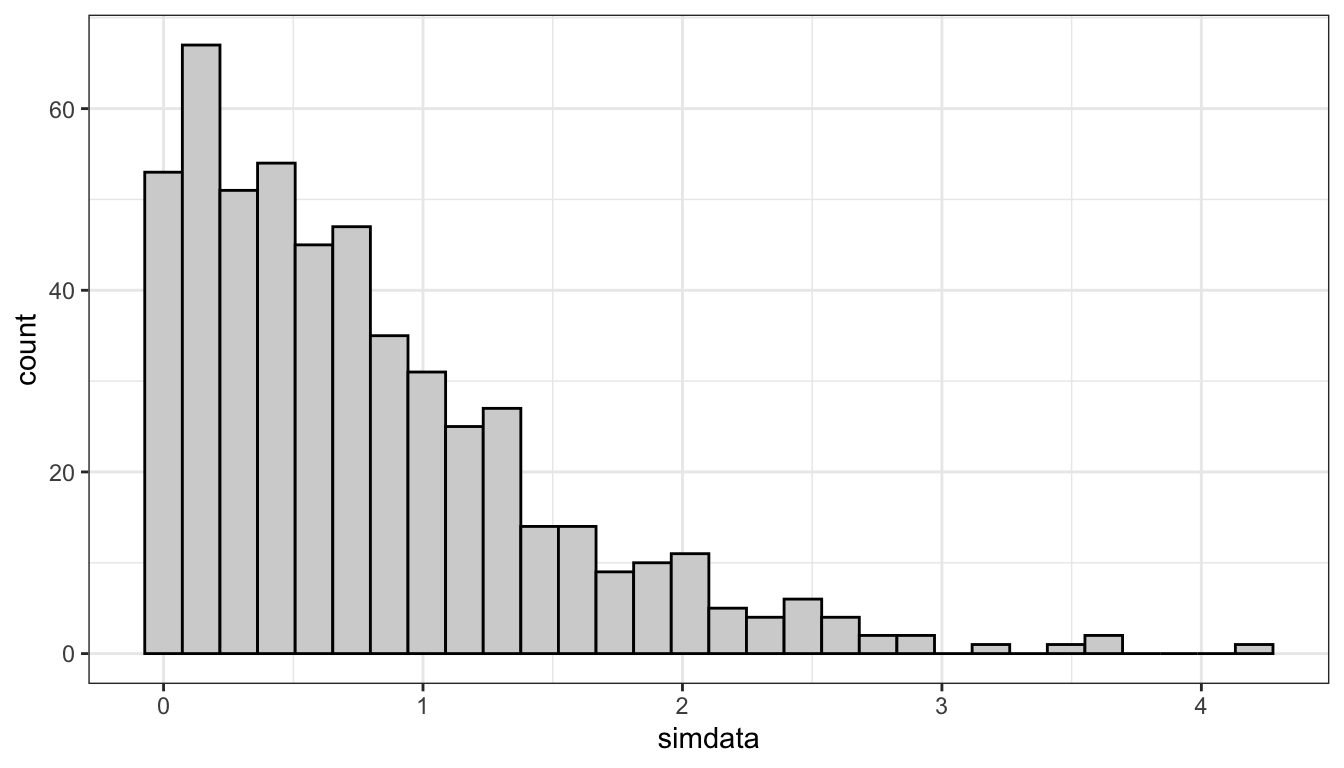
\includegraphics{L01-Intro_PicturingGraphs_files/figure-pdf/unnamed-chunk-17-1.pdf}

}

\end{figure}

---\textgreater{}

\hypertarget{for-next-class}{%
\section{For Next Class!!!}\label{for-next-class}}

\begin{itemize}
\tightlist
\item
  Next class \emph{won't} be a slideshow. It will be closer to active
  learning.\lspace
\item
  Read the notes posted, then we'll expand on the important points in
  class.

  \begin{itemize}
  \tightlist
  \item
    ``Important points'' == ``I will write exam questions about these
    things''\lspace
  \end{itemize}
\item
\end{itemize}

\textbf{Exercises}

\begin{enumerate}
\def\labelenumi{\arabic{enumi}.}
\tightlist
\item
  \textbf{Prescriptions of opioid pain relievers.} Opioid pain relievers
  are prescribed at a higher rate in the United States than in any other
  nation, even though abuse of these medications can result in addiction
  and fatal overdoses. The CDC examined opioid pain reliever
  prescriptions in each state to find out how variable prescription
  rates are across the nation. Here are the 2012 state prescription
  rates, in number of prescriptions per 100 people, listed in increasing
  order:
\end{enumerate}

\texttt{opiods\ \textless{}-\ c(52.0,\ 57.0,\ 59.5,\ 61.6,\ 62.9,\ 65.1,\ 66.5,\ 67.4,\ 67.9,\ 69.6,\ 70.8,\ 71.2,\ 71.7,\ 72.4,\ 72.7,\ 72.8,\ 73.8,\ 74.3,\ 74.3,\ 74.7,\ 76.1,\ 77.3,\ 77.5,\ 79.4,\ 82.0,\ 82.4,\ 85.1,\ 85.6,\ 85.8,\ 88.2,\ 89.2,\ 89.6,\ 90.7,\ 90.8,\ 93.8,\ 94.1,\ 94.8,\ 96.6,\ 100.1,\ 101.8,\ 107.0,\ 109.1,\ 115.8,\ 118.0,\ 120.3,\ 127.8,\ 128.4,\ 137.6,\ 142.8,\ 142.9)}

\begin{enumerate}
\def\labelenumi{\alph{enumi}.}
\tightlist
\item
  Make a histogram of the state opioid pain reliever prescription rates
  using classes of width 10 starting at 50.0 prescriptions per 100
  people. e.g.~(50, 60{]}. Do this by hand first, then using R.
\item
  Would you say that the distribution is single-peaked or
  multiple-peaked? Is it roughly symmetric or skewed?
\end{enumerate}

The Statistical Abstract of the United States, prepared by the Census
Bureau, provides the number of single-organ transplants for the year
2010, by organ. The following two exercises are based on this table:

\begin{longtable}[]{@{}ll@{}}
\toprule\noalign{}
Disease & Count \\
\midrule\noalign{}
\endhead
\bottomrule\noalign{}
\endlastfoot
Heart & 2,333 \\
Lung & 1,770 \\
Liver & 6,291 \\
Kidney & 16,898 \\
Pancreas & 350 \\
Intestine & 151 \\
\end{longtable}

\begin{enumerate}
\def\labelenumi{\arabic{enumi}.}
\setcounter{enumi}{1}
\tightlist
\item
  (1.14 in BM) The data on single-organ transplants can be displayed in
\end{enumerate}

\begin{enumerate}
\def\labelenumi{\alph{enumi}.}
\tightlist
\item
  a pie chart but not a bar graph.
\item
  a bar graph but not a pie chart.
\item
  either a pie chart or a bar graph.
\end{enumerate}

\begin{enumerate}
\def\labelenumi{\arabic{enumi}.}
\setcounter{enumi}{2}
\tightlist
\item
  (1.15 in BM) Kidney transplants represented what percent of single-
  organ transplants in 2010?
\end{enumerate}

\begin{enumerate}
\def\labelenumi{\alph{enumi}.}
\tightlist
\item
  Nearly 61\%.
\item
  One-sixth (nearly 17\%).
\item
  This percent cannot be calculated from the information provided in the
  table.
\end{enumerate}

See also:
\href{https://stats.libretexts.org/Bookshelves/Introductory_Statistics/Book\%3A_OpenIntro_Statistics_(Diez_et_al)./01\%3A_Introduction_to_Data/1.E\%3A_Introduction_to_Data_(Exercises)}{OpenIntro
Textbook} problems relating to visualizations that we have learned,
especially 1.30, 1.36, 1.37, 1.39, 1.40, 1.47.

\hypertarget{describing-distributions-with-numbers}{%
\chapter{Describing Distributions with
Numbers}\label{describing-distributions-with-numbers}}

L02

\hfill\break

\hypertarget{preamble}{%
\chapter{Preamble}\label{preamble}}

\hypertarget{announcements-1}{%
\section{Announcements}\label{announcements-1}}

\begin{itemize}
\tightlist
\item
  A1 is waiting for you!
\end{itemize}

\hypertarget{agenda-1}{%
\section{Agenda}\label{agenda-1}}

\begin{itemize}
\tightlist
\item
  Quantitative Variables\lspace
\item
  Measures of Centre\lspace
\item
  Measures of Spread\lspace
\item
  Graphical displays of summary statistics.\lspace
\item
  Outliers
\end{itemize}

\hypertarget{quantitative-variables-1}{%
\chapter{Quantitative Variables}\label{quantitative-variables-1}}

\hypertarget{parameters-versus-statistics}{%
\section{Parameters Versus
Statistics}\label{parameters-versus-statistics}}

\begin{itemize}
\tightlist
\item
  Numerical summaries are called parameters when they describe an entire
  population, and statistics when they describe a sample\lspace
\item
  Since we typically will not collect data on the entire population, we
  use (sample) statistics to make statements (with some uncertainty)
  about what the (population) parameter is.\lspace
\item
  Categorical variables are summarized by the count or proportion
  (percent) of the data in each category.\lspace
\item
  Quantitative variables are summarized by the centre and spread of the
  data
\end{itemize}

\hypertarget{parameters-versus-statistics-truth}{%
\section{\texorpdfstring{Parameters Versus Statistics:
``\,````Truth''``\,''}{Parameters Versus Statistics: ``\,``\,``Truth''\,``\,''}}\label{parameters-versus-statistics-truth}}

We assume there's some ``true'' population mean.

\begin{itemize}
\tightlist
\item
  This will change if, say, a new baby is born.\lspace
\end{itemize}

\pspace

We cannot know the population parameter!

If we were able to measure the height of every Canadian at this very
instant, we would get one value. We can't do this though, so we collect
a sample instead. We try to collect the sample in such a way that we get
value close to the population parameter.

In this course, we make a big distinction between population parameter
and sample statistic. A sample statistic is something that we calculate
from a sample, where is the population? Parameter is the value that we
would get if we had the whole population.

Most of this course is centred around using the sample statistic to get
an idea of what the population parameter might be.

\hypertarget{measures-of-centre}{%
\chapter{Measures of Centre}\label{measures-of-centre}}

\hypertarget{the-centre}{%
\section{The Centre}\label{the-centre}}

The ``centre'' is a strange concept.

\begin{itemize}
\tightlist
\item
  Where are ``most'' of the data?\lspace
\item
  If we took an individual at random, what's the ``best guess'' of their
  height?\lspace
\end{itemize}

\pspace

We want to \textbf{summarize} the data using a few words/numbers.

I prefer the second description here - if I were to make a prediction, I
want my predicted value to be close to the actual value. For example, I
might want to design something that fits the average person's height. I
must make a prediction about the height of the people that will use it.
My prediction is chosen to minimize how far off I would be, which means
that I want to be near the ``centre''.

\hypertarget{centre-1-the-median}{%
\section{Centre 1: The Median}\label{centre-1-the-median}}

The \textbf{median} (\(M\)) is the midpoint of a distribution: half the
observations are smaller and the other half are larger than it. To find
the median: \pspace

\begin{enumerate}
\def\labelenumi{\arabic{enumi}.}
\tightlist
\item
  Arrange all observations in order of size, from smallest to largest.
\item
  If the number of observations (\(n\)) is odd, the median \(M\) is the
  centre observation in the ordered list. Find the location of the
  median by counting \((n + 1)/2\) observations up from the smallest
  observation.
\item
  If n is even, the median \(M\) halfway between the two centre
  observations in the ordered list. The location of the median is again
  \((n + 1)/2\), counting from the smallest observation in the list.
\end{enumerate}

Basically, the median is the middle value. With odd \(n\), the middle
value is one of the observations, but when \(n\) is even we have to go
in between two values.

\hypertarget{example-1-odd-n}{%
\section{\texorpdfstring{Example 1: Odd
\(n\)}{Example 1: Odd n}}\label{example-1-odd-n}}

The distribution of needle lengths is how species of pine trees are
characterized. The following data are the lengths (in cm) of a sample of
15 needles taken at random from different parts of several Aleppo pine
trees (Southern California). What is the median length?

\begin{verbatim}
7.20 7.60  8.50  8.50  8.70  9.00  9.00 9.30
9.40 9.40 10.20 10.90 11.30 12.10 12.80
\end{verbatim}

\hypertarget{example-2-even-n}{%
\section{\texorpdfstring{Example 2: Even
\(n\)}{Example 2: Even n}}\label{example-2-even-n}}

We also have the lengths (in cm) of 18 needles from trees of the
noticeably different Torrey pine species. What is the median length for
these 18 pine needles? The ordered data are:

\begin{verbatim}
21.20 21.60 21.70 23.10 23.70 24.20 24.20 25.50 26.60
26.80 28.90 29.00 29.70 29.70 30.20 32.50 33.70 33.70
\end{verbatim}

\hypertarget{example-3-robustness}{%
\section{Example 3: Robustness}\label{example-3-robustness}}

\begin{verbatim}
Set 1: 1 2 3 4 5 6
Set 2: 1 1 1 6 6 6
Set 3: -2000 -1000 3 4 5000 60000000
\end{verbatim}

All three have the same median!

\pspace

Do the ``centres'' make sense? Do they provide a good summary?

These three data sets demonstrate that the median only depends on the
middle two numbers when \(n\) is odd. For the first two data sets, the
median does seem to describe centre of the data well. The last data set
is a little bit different from the others and the median might not be
enough information.

\hypertarget{the-mean}{%
\section{The Mean}\label{the-mean}}

The mean is defined as:

\[
\bar x = \frac{1}{n}(x_1 + x_2 + ... + x_n)= \frac{1}{n}\sum_{i=1}^nx_i
\]

For example, the mean of (1, 2, 3, 4) is \[
\frac{1}{4}(1 + 2 + 3 + 4) = \frac{10}{4} = 2.5
\] (this also happens to be the median!)

This formula for the mean may look a little bit scary, but all it means
is that we add up all of the values that we have and divide by the
number of values.

Create a couple examples yourself and find the mean! If you create a
list of values, you can use R to check your work as follows:

\begin{Shaded}
\begin{Highlighting}[]
\NormalTok{my\_values }\OtherTok{\textless{}{-}} \FunctionTok{c}\NormalTok{(}\DecValTok{1}\NormalTok{, }\DecValTok{2}\NormalTok{, }\DecValTok{2}\NormalTok{, }\DecValTok{3}\NormalTok{, }\DecValTok{4}\NormalTok{, }\DecValTok{5}\NormalTok{, }\FloatTok{6.3212}\NormalTok{, }\DecValTok{3}\NormalTok{)}
\FunctionTok{mean}\NormalTok{(my\_values)}
\end{Highlighting}
\end{Shaded}

\begin{verbatim}
[1] 3.29015
\end{verbatim}

\begin{itemize}
\tightlist
\item
  The name ``\texttt{my\_values}'' could have been anything that is just
  letters, numbers, and underscores (no spaces, can't start with a
  number). It's just the name of an object in R.

  \begin{itemize}
  \tightlist
  \item
    An object is just a thing. You can put two things together, do a
    function of a thing, etc.
  \end{itemize}
\item
  \texttt{my\_values} is a \emph{vector}. That is, it's a collection of
  values.

  \begin{itemize}
  \tightlist
  \item
    We create it using the \texttt{c()} function, which means
    ``concatenate'', or ``put together''.
  \end{itemize}
\item
  The mean function takes a vector and calculates the mean for you.
\end{itemize}

To run this code, go to \url{wlu.syzygy.ca} and create a new R notebook.
Insert an ``R cell'', and copy/paste the code above into that cell.
Either hit the ``play'' button, or Alt+Enter (Option+Enter on a Mac).

\hypertarget{the-mean-is-not-robust}{%
\section{\texorpdfstring{The mean is \emph{not}
robust}{The mean is not robust}}\label{the-mean-is-not-robust}}

Consider the following sets of data:

\begin{verbatim}
Set 1: 1, 2, 3, 4, 5, 6
Set 2: 1, 2, 3, 4, 5, 60
\end{verbatim}

\pspace

\begin{itemize}
\tightlist
\item
  Both have the same median.\lspace
\item
  Mean of 3.5 and 12.5, respectively.
\end{itemize}

\pspace

Which do you think is the correct measure of the centre?

Unlike the median, which only depends on the middle value, the mean uses
information from all of the values. This means that if there's an
outlier or a misrecorded point, the mean will reflect this. Sometimes
this is what we want and sometimes it is not.

A common example of when the mean is not what we want is income. The
lowest possible income is zero, but there is no maximum income, so
incomes tend to be right skewed. The right skew affects the mean a lot
more than that affects the median, and so, in this case the median is a
better measure of the most common levels of income.

\hypertarget{mean-and-median-vs.-skew-mean-less-means-left}{%
\section{Mean and Median vs.~Skew: Mean less means
left}\label{mean-and-median-vs.-skew-mean-less-means-left}}

\begin{Shaded}
\begin{Highlighting}[]
\NormalTok{shiny}\SpecialCharTok{::}\FunctionTok{runGitHub}\NormalTok{(}\AttributeTok{repo =} \StringTok{"DBecker7/DB7\_TeachingApps"}\NormalTok{, }
    \AttributeTok{subdir =} \StringTok{"Apps/MeanLessMeansLeft"}\NormalTok{)}
\end{Highlighting}
\end{Shaded}

The app above will be used in class, so do not worry if you're unable to
run it. It demonstrates that when they mean is less than the median it
means it's left skewed. The reason for this is that the outliers to the
left affect the mean more than they affect the median.

\hypertarget{measures-of-spread}{%
\chapter{Measures of Spread}\label{measures-of-spread}}

\hypertarget{which-has-more-variance}{%
\section{Which has more variance?}\label{which-has-more-variance}}

\begin{verbatim}
Set 1: 1 1 1 5 5 5
Set 2: 1 2 3 3 4 5
Set 3: 1 3 3 3 3 5
\end{verbatim}

\pspace

\begin{itemize}
\tightlist
\item
  All have the same \textbf{range} (max - min).
\end{itemize}

These three data sets all have the same mean and median, but just
looking at them shows that they are differnt collections of numbers. The
first said, only has two unique values put those values are relatively
far away from each other compared to the other sets. The second set is a
more even spread from one to five. The third set has for value is equal
to the mean and two values that may be outliers.

To me, the first set looks like it's the most variable because all of
the values are very far away from either the mean or the median. The
second set has a smaller variance, because there are values closer to
the mean. And the last set I expect to have the lowest variance, because
most values are actually equal to the mean.

The formula for the variance, which will introduce next, matches this
intuition. However, many students have different intuitions about which
has the most variance and those are valid as well but are harder to
quantify.

\hypertarget{measure-of-spread-the-variance}{%
\section{Measure of Spread: The
Variance}\label{measure-of-spread-the-variance}}

Consider set 1, which has a mean of 3:

\begin{verbatim}
1 1 1 5 5 5
\end{verbatim}

\begin{itemize}
\tightlist
\item
  The distances to the mean are all -2 or 2

  \begin{itemize}
  \tightlist
  \item
    If we found the mean, we'd get 0! We need to make sure they're all
    positive.\lspace
  \end{itemize}
\item
  Alternative 1: Absolute value. The average \emph{absolute} distance to
  the mean is 2.\lspace
\item
  Alternative 2: Squared value.

  \begin{itemize}
  \tightlist
  \item
    The \textbf{average squared distance to the mean} is 4

    \begin{itemize}
    \tightlist
    \item
      Important: This is not the actual variance calculation!
    \end{itemize}
  \end{itemize}
\end{itemize}

The \textbf{variance} is the average \emph{squared} distance to the
mean!

(We use squared because math - more on this later).

We are basically looking at the average deviation from the mean. We want
that deviation to be positive and there are several ways to do this. We
have settled on squaring the numbers for the same reason we drive on the
right side of the road: it's just convention. There are benefits to
using the absolute distance from the mean, but there are many
mathematical advantages to squaring the values first.

\hypertarget{variance-formula}{%
\section{Variance Formula}\label{variance-formula}}

\vspace{1.5cm}

\[
s^2 = \frac{1}{n-1}\sum_{i=1}^n(x_i - \bar x)^2
\]

\pspace

We use \(n-1\) because of math reasons.

The easiest way to calculate this is to put it in a table:

\begin{longtable}[]{@{}llll@{}}
\toprule\noalign{}
\(i\) & \(x_i\) & \(x_i - \bar x\) & \((x_i - \bar x)^2\) \\
\midrule\noalign{}
\endhead
\bottomrule\noalign{}
\endlastfoot
1 & 1 & -2 & 4 \\
2 & 1 & -2 & 4 \\
3 & 1 & -2 & 4 \\
4 & 5 & 2 & 4 \\
5 & 5 & 2 & 4 \\
6 & 5 & 2 & 4 \\
\(\sum\) & 18 & 0 & 24 \\
\end{longtable}

The mean is 3, and the variance is 24/5 = 4.8.

In the table above, as before, the subscript \(i\) is just used to
denote different observations. For example \(x_1\) is the first
observation, \(x_2\) is the second observation in our data, and so on
(this ordering is arbitrary).

In order to calculate the variance, we must first know the mean, and so
it's convenient to put this at the bottom of the table. We then squared
the deviations from the mean and divided by \(n-1\). There are very good
technical reasons why we divide by (n-1) that we won't get into here.
Come to my office and chat if you'd like to know more, or just ask
ChatGPT!

\begin{tcolorbox}[enhanced jigsaw, opacitybacktitle=0.6, left=2mm, colbacktitle=quarto-callout-note-color!10!white, colframe=quarto-callout-note-color-frame, breakable, toptitle=1mm, title=\textcolor{quarto-callout-note-color}{\faInfo}\hspace{0.5em}{\(n-1\) in the denominator}, opacityback=0, bottomrule=.15mm, toprule=.15mm, arc=.35mm, leftrule=.75mm, titlerule=0mm, bottomtitle=1mm, colback=white, rightrule=.15mm, coltitle=black]

As a quick explanation for \(n-1\), consider the variance of a single
observation. It doesn't vary! There's not enough information to see how
much variance there is. There isn't enough \emph{information} in our
data. The \(n-1\) in the denominator enforces this - we can't calculate
the variance of one observation.

\end{tcolorbox}

Note that the variance can be calculated in R as follows:

\begin{Shaded}
\begin{Highlighting}[]
\NormalTok{my\_values }\OtherTok{\textless{}{-}} \FunctionTok{c}\NormalTok{(}\DecValTok{1}\NormalTok{, }\DecValTok{2}\NormalTok{, }\DecValTok{2}\NormalTok{, }\DecValTok{3}\NormalTok{, }\DecValTok{4}\NormalTok{, }\DecValTok{5}\NormalTok{, }\FloatTok{6.3212}\NormalTok{, }\DecValTok{3}\NormalTok{)}
\FunctionTok{var}\NormalTok{(my\_values)}
\end{Highlighting}
\end{Shaded}

\begin{verbatim}
[1] 3.050982
\end{verbatim}

\hypertarget{the-variance-and-the-standard-deviation}{%
\section{The Variance and the Standard
Deviation}\label{the-variance-and-the-standard-deviation}}

\[
s = \sqrt{\frac{1}{n-1}\sum_{i=1}^n(x - \bar x)^2}
\]

The \textbf{standard deviation} (or \textbf{sd}) is just the square root
of the variance.

\begin{itemize}
\tightlist
\item
  This makes it have the same units as the original data.
\end{itemize}

In addition, if we have two data sets and the variance of one is larger
than the other, then the standard deviation is also larger. They're the
same thing, just in different units!

I will often refer to one when I mean the other. When I'm comparing
standard deviations, I may call them variances because the same patterns
will be there.

Here's the R code:

\begin{Shaded}
\begin{Highlighting}[]
\FunctionTok{sd}\NormalTok{(my\_values)}
\end{Highlighting}
\end{Shaded}

\begin{verbatim}
[1] 1.746706
\end{verbatim}

\begin{Shaded}
\begin{Highlighting}[]
\FunctionTok{sd}\NormalTok{(my\_values)}\SpecialCharTok{\^{}}\DecValTok{2} \CommentTok{\# the sd is the square root of the variance}
\end{Highlighting}
\end{Shaded}

\begin{verbatim}
[1] 3.050982
\end{verbatim}

\hypertarget{exercise-variation-of-the-three-sets}{%
\section{Exercise: Variation of the three
sets}\label{exercise-variation-of-the-three-sets}}

\begin{verbatim}
Set 1: 1 1 1 5 5 5
Set 2: 1 2 3 3 4 5
Set 3: 1 3 3 3 3 5
\end{verbatim}

\pspace

\begin{enumerate}
\def\labelenumi{\arabic{enumi}.}
\tightlist
\item
  Draw out bar plots.\lspace
\item
  Set up the table and find the variance.\lspace
\item
  Compare the standard deviations; make a conclusion.
\end{enumerate}

\begin{longtable}[]{@{}llll@{}}
\toprule\noalign{}
\(i\) & \(x_i\) & \(x_i - \bar x\) & \((x_i - \bar x)^2\) \\
\midrule\noalign{}
\endhead
\bottomrule\noalign{}
\endlastfoot
1 & & & \\
2 & & & \\
3 & & & \\
4 & & & \\
5 & & & \\
6 & & & \\
\(\sum\) & & & \\
\end{longtable}

Fill out the table above yourself!

\hypertarget{measure-of-spread-2-the-iqr}{%
\section{Measure of Spread 2: The
IQR}\label{measure-of-spread-2-the-iqr}}

The IQR is very closely related to the median. But first, we will learn
what quartiles are.

Consider the data:

\begin{verbatim}
1 2 3 4 5 6 7 8
\end{verbatim}

The median of these data is 5; 50\% of the data are to the left of this
point.

\begin{itemize}
\tightlist
\item
  ``Quartile'': Split the data into four.

  \begin{itemize}
  \tightlist
  \item
    Q1: 25\% of the data are to the left.
  \item
    Q2: 50\% of the data are to the left (the median).
  \item
    Q3: 75\% of the data are to the left.
  \end{itemize}
\end{itemize}

\hypertarget{finding-quartiles}{%
\section{Finding Quartiles}\label{finding-quartiles}}

\begin{verbatim}
1 2 3 4 5 6 7 8
\end{verbatim}

\begin{enumerate}
\def\labelenumi{\arabic{enumi}.}
\tightlist
\item
  Find the median

  \begin{itemize}
  \tightlist
  \item
    It's 4.5. Cool.
  \end{itemize}
\item
  Q1 is just half of 50\% - we're finding a median again!

  \begin{itemize}
  \tightlist
  \item
    Q1 is the median of everything to the left of the median.
  \item
    In this case, 1 2 3 4 are the numbers to the left of the median, and
    so Q1 is 2.5.
  \end{itemize}
\item
  By a similar argument, Q3 is 6.5.
\end{enumerate}

Q0 is where 0\% of the data are to the left. In other words, it's the
minimum value in the data! Similarly, Q4 is the maximum value in the
data.

\begin{tcolorbox}[enhanced jigsaw, opacitybacktitle=0.6, left=2mm, colbacktitle=quarto-callout-warning-color!10!white, colframe=quarto-callout-warning-color-frame, breakable, toptitle=1mm, title=\textcolor{quarto-callout-warning-color}{\faExclamationTriangle}\hspace{0.5em}{Warning}, opacityback=0, bottomrule=.15mm, toprule=.15mm, arc=.35mm, leftrule=.75mm, titlerule=0mm, bottomtitle=1mm, colback=white, rightrule=.15mm, coltitle=black]

The algorithm we just used for computing the quartiles is not the only
one! In R, there are \emph{NINE} different ways to calculate the
quartiles. You should stick to doing this by hand if you want to get the
WeBWork answers right.

\end{tcolorbox}

\hypertarget{the-five-number-summary}{%
\section{The five number summary}\label{the-five-number-summary}}

Let's use the folowing example:

\begin{verbatim}
1, 3, 3, 4, 5, 5, 5, 6, 7, 7, 8, 8, 9, 10, 10, 11, 12
\end{verbatim}

The quartiles give an excellent way to summarise data:

\begin{longtable}[]{@{}lllll@{}}
\toprule\noalign{}
Q0 (min) & Q1 & Q2 (median) & Q3 & Q4 (max) \\
\midrule\noalign{}
\endhead
\bottomrule\noalign{}
\endlastfoot
1 & 4.5 & 7 & 8.5 & 12 \\
\end{longtable}

The five number summary just shows all five of the quartiles. Note that
there are five quartiles, because zero is also one of them.

For practice, make sure you can calculate the median, and then the
median of all the values to the left of it!

\hypertarget{visualizing-the-five-number-summary-the-boxplot}{%
\section{Visualizing the five number summary: the
boxplot}\label{visualizing-the-five-number-summary-the-boxplot}}

\vspace{1cm}

The plot on the right shows the body masses for the Palmer Penguins.

\pspace

\begin{itemize}
\tightlist
\item
  The lowest point is Q0
\item
  The left of the box is Q1
\item
  The thick line in the box is Q2 (the median)
\item
  The right of the box is Q3
\item
  The highest point is Q4
\end{itemize}

\begin{Shaded}
\begin{Highlighting}[]
\FunctionTok{library}\NormalTok{(ggplot2)}
\FunctionTok{library}\NormalTok{(palmerpenguins)}
\FunctionTok{theme\_set}\NormalTok{(}\FunctionTok{theme\_bw}\NormalTok{())}

\FunctionTok{ggplot}\NormalTok{(penguins) }\SpecialCharTok{+} 
    \FunctionTok{aes}\NormalTok{(}\AttributeTok{y =}\NormalTok{ body\_mass\_g) }\SpecialCharTok{+}
    \FunctionTok{geom\_boxplot}\NormalTok{() }\SpecialCharTok{+}
    \FunctionTok{labs}\NormalTok{(}\AttributeTok{y =} \StringTok{"Body Mass (g)"}\NormalTok{) }\SpecialCharTok{+}
    \FunctionTok{coord\_flip}\NormalTok{()}
\end{Highlighting}
\end{Shaded}

\begin{figure}[H]

{\centering \includegraphics{L02-Describing_Distributions_Numbers_files/figure-pdf/unnamed-chunk-5-1.pdf}

}

\end{figure}

\begin{Shaded}
\begin{Highlighting}[]
\FunctionTok{ggplot}\NormalTok{(penguins) }\SpecialCharTok{+} 
    \FunctionTok{aes}\NormalTok{(}\AttributeTok{x =}\NormalTok{ body\_mass\_g) }\SpecialCharTok{+}
    \FunctionTok{geom\_histogram}\NormalTok{(}\AttributeTok{colour =} \DecValTok{1}\NormalTok{, }\AttributeTok{fill =} \StringTok{"lightgrey"}\NormalTok{) }\SpecialCharTok{+}
    \FunctionTok{labs}\NormalTok{(}\AttributeTok{x =} \StringTok{"Body Mass (g)"}\NormalTok{)}
\end{Highlighting}
\end{Shaded}

\begin{figure}[H]

{\centering \includegraphics{L02-Describing_Distributions_Numbers_files/figure-pdf/unnamed-chunk-6-1.pdf}

}

\end{figure}

The boxplot and the histogram both demonstrate the right skew of the
data, but the boxplot is much more compact!

Take a moment to compare the two plots and make sure you can explain the
skewness. Remember that 25\% of the data are in each interval shown in
the box plot!

\hypertarget{measure-2-the-inter-quartile-range-iqr}{%
\section{Measure 2: The Inter-Quartile Range
(IQR)}\label{measure-2-the-inter-quartile-range-iqr}}

The IQR is defined as: Q3 - Q1.

\pspace

\begin{itemize}
\tightlist
\item
  Same units as the original data\lspace
\item
  Robust to outliers (unlike the sd)!
\end{itemize}

This is the second measure of spread that we will learn. The IQR is
commonly used when we have highly skewed data or data with outliers. The
sd measures the average squared deviation from the mean, whereas the IQR
measures the middle 50\% of the data.

Notice how this is not centered on the median. Consider the following
data:

\begin{Shaded}
\begin{Highlighting}[]
\NormalTok{my\_values }\OtherTok{\textless{}{-}} \FunctionTok{c}\NormalTok{(}\DecValTok{1}\NormalTok{, }\DecValTok{1}\NormalTok{, }\DecValTok{1}\NormalTok{, }\DecValTok{2}\NormalTok{, }\DecValTok{2}\NormalTok{, }\DecValTok{2}\NormalTok{, }\DecValTok{2}\NormalTok{, }\DecValTok{3}\NormalTok{, }\DecValTok{3}\NormalTok{, }\DecValTok{3}\NormalTok{, }\DecValTok{3}\NormalTok{, }\DecValTok{3}\NormalTok{, }\DecValTok{4}\NormalTok{, }\DecValTok{4}\NormalTok{, }\DecValTok{4}\NormalTok{, }\DecValTok{5}\NormalTok{, }\DecValTok{6}\NormalTok{, }\DecValTok{7}\NormalTok{, }\DecValTok{8}\NormalTok{, }\DecValTok{10}\NormalTok{)}
\FunctionTok{length}\NormalTok{(my\_values)}
\end{Highlighting}
\end{Shaded}

\begin{verbatim}
[1] 20
\end{verbatim}

\begin{Shaded}
\begin{Highlighting}[]
\FunctionTok{hist}\NormalTok{(my\_values)}
\end{Highlighting}
\end{Shaded}

\begin{figure}[H]

{\centering \includegraphics{L02-Describing_Distributions_Numbers_files/figure-pdf/unnamed-chunk-7-1.pdf}

}

\end{figure}

The median of these should be at position
\((n+1)/2 = (20 + 1)/2 = 10.5\) (I used the \texttt{length()} function
in R to count the number of observations for me). This value is halfway
between 3 and 3, meaning it's 3. Q1 is the median of the first 10 data
points, which is at position 5.5, giving us a value of 2. Q3 is 5.5
positions from the end, which is 4.5. Thus the IQR is \(4.5 - 2 = 2.5\).

First, does this make sense to you? Does 2.5 sound like a reasonable
width for the middle 50\%?

Now consider that the distribution is clearly skewed to the right. This
affects the variance a lot, but the IQR would have been the same no
matter what the first 4 or last 4 values were.

\hypertarget{iqr-for-outliers}{%
\section{IQR for Outliers}\label{iqr-for-outliers}}

In this class, we use a rule of thumb for calculating outliers. Anything
that is\ldots{}

\begin{itemize}
\tightlist
\item
  Below the median minus 1.5*IQR, or
\item
  above the median plus 1.5*IQR
\end{itemize}

is considered an outlier.

This rule of thumb is not based on any mathematical derivations, it just
seems to work in most situations.

The idea is that the IQR gives a measure of spread, and the median gives
the measure of the centre, so anything too far from the centre is an
outlier. We use the spread to figure out how far away from the centre we
are willing to accept. This will show up several times in this course.
We've seen it in this example for the IQR and median because this is
simple and easy to interpret.

Most of the rest of this course will be spent looking at something
similar for the mean. We will still use this idea of the centre plus or
minus some measure of the spread, but will incorporate information about
the sample and assumptions about the population that allow us to make
much stronger conclusions beyond simply checking if something is an
outlier.

\hypertarget{summary-1}{%
\section{Summary}\label{summary-1}}

\begin{itemize}
\tightlist
\item
  The ``centre'' is trying to measure the most common value.

  \begin{itemize}
  \tightlist
  \item
    Often, this is our best \textbf{prediction}.\lspace
  \end{itemize}
\item
  The ``spread'' is trying to measure the scale, or variation.

  \begin{itemize}
  \tightlist
  \item
    Gives context to the centre.\lspace
  \end{itemize}
\item
  The mean and variance

  \begin{itemize}
  \tightlist
  \item
    Interpretations and formulas are important.\lspace
  \end{itemize}
\item
  The median and IQR

  \begin{itemize}
  \tightlist
  \item
    Calculations, interpretations, five-number-summary, outliers, and
    boxplots are all important.
  \end{itemize}
\end{itemize}

We saw the same thing a couple of times throughout this lesson. We saw
measures of centre that try to describe the middle of a distribution and
centres of spread that tell us how spread out the data are. The mean and
the sd are intrinsically linked, and the median and IQR are
intrinsically linked.

We also saw the rule-of-thumb to use IQR for finding outliers by using
the median plus-an-minus some number times the spread. You better
believe that this idea will show up again later in this course!

Boxplots are a visual representation of the five number summary. These
can be very small while still showing the shape of our data. However,
these only work for unimodal data - there isn't a good way to show a
bimodal distribution on a boxplot. Also, it is very easy to plot two
boxplots for two different data sets in order to compare the
distributions.

For assignments and exams, be ready to calculate any of these values and
compare the mean/median and sd/IQR. Also be ready to compare the five
number summary to a boxplot.

\textbf{Exercises}

\begin{enumerate}
\def\labelenumi{\arabic{enumi}.}
\tightlist
\item
  \textbf{Spider Silk.} Spider silk is the strongest known material,
  natural or man-made, on a weight basis. A study examined the
  mechanical properties of spider silk using 21 female golden orb
  weavers, Nephila clavipes. Here are data on silk yield stress, which
  represents the amount of force per unit area needed to reach permanent
  deformation of the silk strand. The data are expressed in megapascals
  (MPa):
\end{enumerate}

\begin{verbatim}
164.00 173.00 176.10 236.10 251.30 270.50 270.50
272.40 282.20 288.80 290.70 300.60 327.20 329.00
332.10 351.70 358.20 362.00 448.90 478.70 740.20
\end{verbatim}

\begin{enumerate}
\def\labelenumi{\alph{enumi}.}
\tightlist
\item
  Describe the shape, centre, and spread of the data using a histogram
  (code below).
\item
  Find the mean and median yield stress. Compare these two values.
  Referring to the histogram produced by the code below, what general
  fact does your comparison illustrate?
\item
  Re-run the code using different values of \texttt{breaks}. What do you
  see? (Note that this example uses base R rather than \texttt{ggplot2}
  because it has simpler code - \texttt{ggplot2} has more flexibility,
  but that flexibility isn't necessary here.)
\item
  Use the \texttt{boxplot()} function to create a boxplot (you do not
  need the \texttt{breaks=10} part of the code). Compare this to the
  histogram. Also comment on any points that stand out (when there are
  outliers, R shows \(Q2\pm 1.5IQR\) rather than Q0 and Q4).
\item
  Use the \(Q2\pm 1.5IQR\) formula by hand to find the outliers, and
  verify your calculations with the R plot.
\end{enumerate}

\begin{Shaded}
\begin{Highlighting}[]
\NormalTok{silk\_stress }\OtherTok{\textless{}{-}} \FunctionTok{c}\NormalTok{(}\FloatTok{164.00}\NormalTok{, }\FloatTok{173.00}\NormalTok{, }\FloatTok{176.10}\NormalTok{, }\FloatTok{236.10}\NormalTok{, }\FloatTok{251.30}\NormalTok{, }\FloatTok{270.50}\NormalTok{, }\FloatTok{270.50}\NormalTok{,}
    \FloatTok{272.40}\NormalTok{, }\FloatTok{282.20}\NormalTok{, }\FloatTok{288.80}\NormalTok{, }\FloatTok{290.70}\NormalTok{, }\FloatTok{300.60}\NormalTok{, }\FloatTok{327.20}\NormalTok{, }\FloatTok{329.00}\NormalTok{,}
    \FloatTok{332.10}\NormalTok{, }\FloatTok{351.70}\NormalTok{, }\FloatTok{358.20}\NormalTok{, }\FloatTok{362.00}\NormalTok{, }\FloatTok{448.90}\NormalTok{, }\FloatTok{478.70}\NormalTok{, }\FloatTok{740.20}\NormalTok{)}
\FunctionTok{hist}\NormalTok{(silk\_stress, }\AttributeTok{breaks =} \DecValTok{10}\NormalTok{)}
\end{Highlighting}
\end{Shaded}

\begin{figure}[H]

{\centering \includegraphics{L02-Describing_Distributions_Numbers_files/figure-pdf/unnamed-chunk-8-1.pdf}

}

\end{figure}

\begin{enumerate}
\def\labelenumi{\arabic{enumi}.}
\setcounter{enumi}{1}
\item
  \textbf{Deep-sea sediments.} Phytopigments are markers of the amount
  of organic matter that settles in sediments on the ocean floor.
  Phytopigment concentrations in deep-sea sediments collected worldwide
  showed a very strong right-skew. Of two summary statistics, 0.015 and
  0.009 gram per square meter of bottom surface, which one is the mean
  and which one is the median? Explain your reasoning.
\item
  \textbf{Glucose levels.} People with diabetes must monitor and control
  their blood glucose level. The goal is to maintain a ``fasting plasma
  glucose'' between approximately 90 and 130 milligrams per deciliter
  (mg/dl). The data tables below give the fasting plasma glucose levels
  for two groups of diabetics five months after they received either
  group instruction or individual instruction on glucose control.
\end{enumerate}

I provide the data as vectors in R, but you don't need R for this
question (it's good practice to do it both ways).

\begin{Shaded}
\begin{Highlighting}[]
\NormalTok{group }\OtherTok{\textless{}{-}} \FunctionTok{c}\NormalTok{(}\FloatTok{78.00}\NormalTok{, }\FloatTok{95.00}\NormalTok{, }\FloatTok{96.00}\NormalTok{, }\FloatTok{103.00}\NormalTok{, }\FloatTok{112.00}\NormalTok{, }\FloatTok{134.00}\NormalTok{, }\FloatTok{141.00}\NormalTok{, }\FloatTok{145.00}\NormalTok{, }\FloatTok{147.00}\NormalTok{,}
    \FloatTok{148.00}\NormalTok{, }\FloatTok{153.00}\NormalTok{, }\FloatTok{158.00}\NormalTok{, }\FloatTok{172.00}\NormalTok{, }\FloatTok{172.00}\NormalTok{, }\FloatTok{200.00}\NormalTok{, }\FloatTok{255.00}\NormalTok{, }\FloatTok{271.00}\NormalTok{, }\FloatTok{359.00}\NormalTok{)}

\NormalTok{individual }\OtherTok{\textless{}{-}} \FunctionTok{c}\NormalTok{(}\FloatTok{128.00}\NormalTok{, }\FloatTok{128.00}\NormalTok{, }\FloatTok{158.00}\NormalTok{, }\FloatTok{159.00}\NormalTok{, }\FloatTok{160.00}\NormalTok{, }\FloatTok{163.00}\NormalTok{, }\FloatTok{164.00}\NormalTok{, }\FloatTok{188.00}\NormalTok{, }\FloatTok{195.00}\NormalTok{,}
    \FloatTok{198.00}\NormalTok{, }\FloatTok{220.00}\NormalTok{, }\FloatTok{221.00}\NormalTok{, }\FloatTok{223.00}\NormalTok{, }\FloatTok{226.00}\NormalTok{, }\FloatTok{227.00}\NormalTok{, }\FloatTok{283.00}\NormalTok{)}
\end{Highlighting}
\end{Shaded}

\begin{enumerate}
\def\labelenumi{\alph{enumi}.}
\tightlist
\item
  Calculate the five-number summary for each of the two data sets.
\item
  Make side-by-side boxplots comparing the two groups. What can you say
  from this graph about the differences between the two diabetes control
  instruction methods? (\emph{Hint, you can create side-by-side boxplot
  using the code \texttt{boxplot(variable\_1,\ variable\_2)}}.)
\item
  Obtain the mean and standard deviation for each sample. Does this
  information give any clue about the shape of the two distributions?
\item
  Add to the historgrams a symbol representing the mean of each group
  and error bars representing one standard deviation above and below the
  mean. (You can do this by hand.) Compare this graphical summary with
  the boxplot display you also created.
\item
  Use the 1.5 × IQR rule to identify any suspected outliers. Then look
  at the raw data to determine if unusually high or low values in either
  data set actually are outliers.
\end{enumerate}

\hypertarget{scatterplots-and-correlation}{%
\chapter{Scatterplots and
Correlation}\label{scatterplots-and-correlation}}

\hypertarget{preamble-1}{%
\chapter{Preamble}\label{preamble-1}}

\hypertarget{announcements-2}{%
\section{Announcements}\label{announcements-2}}

\begin{itemize}
\tightlist
\item
  Lab today!\lspace
\item
  WeBWork A2 out soon.\lspace
\end{itemize}

\hypertarget{agenda-2}{%
\section{Agenda}\label{agenda-2}}

\begin{itemize}
\tightlist
\item
  Relationships\lspace
\item
  Plots (Scatterplots)\lspace
\item
  Numbers (Correlation)
\end{itemize}

\hypertarget{relationships}{%
\chapter{Relationships}\label{relationships}}

\hypertarget{explanatory-and-response-variables}{%
\section{Explanatory and Response
Variables}\label{explanatory-and-response-variables}}

\begin{itemize}
\tightlist
\item
  \textbf{Response:} Responds to the explanatory variable.

  \begin{itemize}
  \tightlist
  \item
    Also called \textbf{dependent} variable.\lspace
  \end{itemize}
\item
  \textbf{Explanatory:} Explains the response variable.

  \begin{itemize}
  \tightlist
  \item
    Also called \textbf{independent} variable.
  \end{itemize}
\end{itemize}

Knowledge about explanatory tells us about the response.

\pspace\pause

\begin{itemize}
\tightlist
\item
  We are \emph{not} assuming the explanatory causes the response. We
  will \emph{not} be covering causality in this course.\lspace
\item
  We are discovering tendencies, \emph{not} rules.
\end{itemize}

I just want to make this very clear: we are not looking for a causation.
Instead, we're just looking at whether or not to variables are related,
and we think that measurements of one will be enough to tell us about
measurements of the other. For example, if we think one variable is easy
to measure and another is harder to measure, then we might want to set
the easy to measure variable as the explanatory variable and see if it
``explains'' the harder to measure variable. This has nothing to do with
the easy to measure variable causing the hard to measure one.

\hypertarget{examples}{%
\section{Examples}\label{examples}}

\begin{itemize}
\tightlist
\item
  Blood alcohol content affects reflex time. -- Some individuals may be
  more or less affected.\lspace
\item
  Smoking cigarettes is associated with increased risk of lung cancer,
  and mortality. -- Some heavy smokers may live to age 90\lspace
\item
  As height increases, weight tends to increase.

  \begin{itemize}
  \tightlist
  \item
    Height does cause weight, but there are other explanations.
  \end{itemize}
\end{itemize}

In these examples, we carefully use words like ``affects'', ``associated
with'', and ``tends to''. For all of these examples we would expect a
relationship of some sort, but the causality is not necessarily obvious.

We obviously expect the blood alcohol contact to affect reflex time. We
expect this to be a causal relationship.

In the mid-1900s, it was hypothesized by cigarette companies that,
rather than cigarettes causing cancer, people who were at increased risk
of lung cancer with the sorts of people who also tended to smoke.
Finding a relationship was not enough to convince people that it was
cigarettes causing lung cancer. Even though we know that there's a
relationship between cigarettes and lung cancer, the techniques we learn
in this course are not enough to conclude causality.

Height and weight are an example of how are the knowledge of one
variable tells us about the other, without there being any causal
relationship. We expect that taller people will have more mass, but
there are also other reasons why somebody might have more mass that or
not captured by their height.

\hypertarget{scatterplots}{%
\chapter{Scatterplots}\label{scatterplots}}

\hypertarget{example}{%
\section{Example}\label{example}}

\includegraphics[width=0.5\textwidth]{figs/manatee1.png}

\includegraphics[width=0.5\textwidth]{figs/manatee2.png}

In the data frame above, we have an observation of the number of power
boats registered in each year, as well as the number of manatees that
died in a collision with a powerboat in that year. The table shown above
is only a small part of the data.

The rest of the data are shown in the plot. To create this plot, we put
the number of powerboats registered on the X axis, and the number of
manatee deaths on the Y axis. The annotation on the plot demonstrates
how the points were added. One of the columns in the data is labelled
1977 and in that year they were to 755,000 powerboats registered and
they were 54 manatee deaths that year. Because these two numbers are
measured on the same individual (with the individual being the year in
this example), we know that those two numbers go together. If we had a
collection of peoples heights and a separate collection of peoples
weights, but no knowledge of which individual each was collected on,
then we would not be able to make a scatterplot. In order to make a
scatterplot, we have to know which observation on the X axis is
associated with which observation on the Y axis.

\hypertarget{what-to-look-for}{%
\section{What to look for}\label{what-to-look-for}}

\pspace

\begin{itemize}
\tightlist
\item
  \textbf{Overall pattern}

  \begin{itemize}
  \tightlist
  \item
    Linear, curved, etc.
  \item
    \textbf{Direction} (increasing/\textbf{positive},
    decreasing/\textbf{negative})
  \item
    Constant variability\lspace
  \end{itemize}
\item
  \textbf{Deviations} from the pattern

  \begin{itemize}
  \tightlist
  \item
    E.g., linear only in a small range\lspace
  \end{itemize}
\item
  \textbf{Outliers}

  \begin{itemize}
  \tightlist
  \item
    As before, discuss outliers separately from the pattern.
  \end{itemize}
\end{itemize}

\includegraphics[width=0.5\textwidth]{figs/manatee2.png}

In general for this course were looking for a linear pattern. There are
other models out there that fit nonlinear patterns, but we do not cover
them in this course. There's one way for things to be linear, and there
are an infinite number of ways for things to be nonlinear. However,
there are many common ways to account for non-linearity while still
using a linear model.

Regardless of whether something is linear or has some sort of curve, we
are very interested in how strong of a pattern there is. For a linear
model this means we want the points to be very close to the line,
whereas for non-linear models we want the pattern to be very clear. We
generally want patterns to pass the ``facial impact test'', were the
pattern is so obvious that it might as well be slapping you in the face
(this is not an official test).

As with describing the shape of histograms, we treat outliers as
something that are not part of the shape. We can have a clear linear
pattern that happens to have an outlier.

The plot of manatees versus powerboats above would be described as a
strong linear pattern, perhaps with some extra variation at larger X
values.

\hypertarget{penguins}{%
\section{Penguins!}\label{penguins}}

\vspace{1cm}

What pattern is this?

\begin{Shaded}
\begin{Highlighting}[]
\FunctionTok{library}\NormalTok{(palmerpenguins)}
\FunctionTok{library}\NormalTok{(ggplot2)}
\FunctionTok{theme\_set}\NormalTok{(}\FunctionTok{theme\_bw}\NormalTok{())}

\FunctionTok{ggplot}\NormalTok{(penguins) }\SpecialCharTok{+} 
    \FunctionTok{aes}\NormalTok{(}\AttributeTok{x =}\NormalTok{ flipper\_length\_mm, }\AttributeTok{y =}\NormalTok{ body\_mass\_g) }\SpecialCharTok{+}
    \FunctionTok{geom\_point}\NormalTok{() }\SpecialCharTok{+} 
    \FunctionTok{geom\_smooth}\NormalTok{(}\AttributeTok{formula =}\NormalTok{ y}\SpecialCharTok{\textasciitilde{}}\NormalTok{x, }\AttributeTok{method =} \StringTok{"lm"}\NormalTok{, }\AttributeTok{se =} \ConstantTok{FALSE}\NormalTok{) }\SpecialCharTok{+}
    \FunctionTok{labs}\NormalTok{(}\AttributeTok{x =} \StringTok{"Flipper Length (mm)"}\NormalTok{,}
        \AttributeTok{y =} \StringTok{"Body Mass (g)"}\NormalTok{)}
\end{Highlighting}
\end{Shaded}

\begin{figure}[H]

{\centering \includegraphics{L03-Scatterplots_Correlation_files/figure-pdf/unnamed-chunk-1-1.pdf}

}

\end{figure}

The plot above shows a clear linear pattern. There is still some
variation above and below the lines, but the pattern is still clear. It
kinda looks like there may be two clusters; there's a space between the
two groups in the center of the X axis.

\hypertarget{adding-a-categorical-variable}{%
\section{Adding a Categorical
Variable}\label{adding-a-categorical-variable}}

\vspace{1cm}

Each point has an \(x\) coordinate, \(y\) coordinate, and some other
information.

\pspace

We can encode that information with a colour!

\begin{Shaded}
\begin{Highlighting}[]
\FunctionTok{library}\NormalTok{(palmerpenguins)}
\FunctionTok{library}\NormalTok{(ggplot2)}
\FunctionTok{theme\_set}\NormalTok{(}\FunctionTok{theme\_bw}\NormalTok{())}

\FunctionTok{ggplot}\NormalTok{(penguins) }\SpecialCharTok{+} 
    \FunctionTok{aes}\NormalTok{(}\AttributeTok{x =}\NormalTok{ flipper\_length\_mm, }\AttributeTok{y =}\NormalTok{ body\_mass\_g,}
        \AttributeTok{colour =}\NormalTok{ species) }\SpecialCharTok{+}
    \FunctionTok{geom\_point}\NormalTok{() }\SpecialCharTok{+}
    \FunctionTok{labs}\NormalTok{(}\AttributeTok{x =} \StringTok{"Flipper Length (mm)"}\NormalTok{,}
        \AttributeTok{y =} \StringTok{"Body Mass (g)"}\NormalTok{)}
\end{Highlighting}
\end{Shaded}

\begin{figure}[H]

{\centering 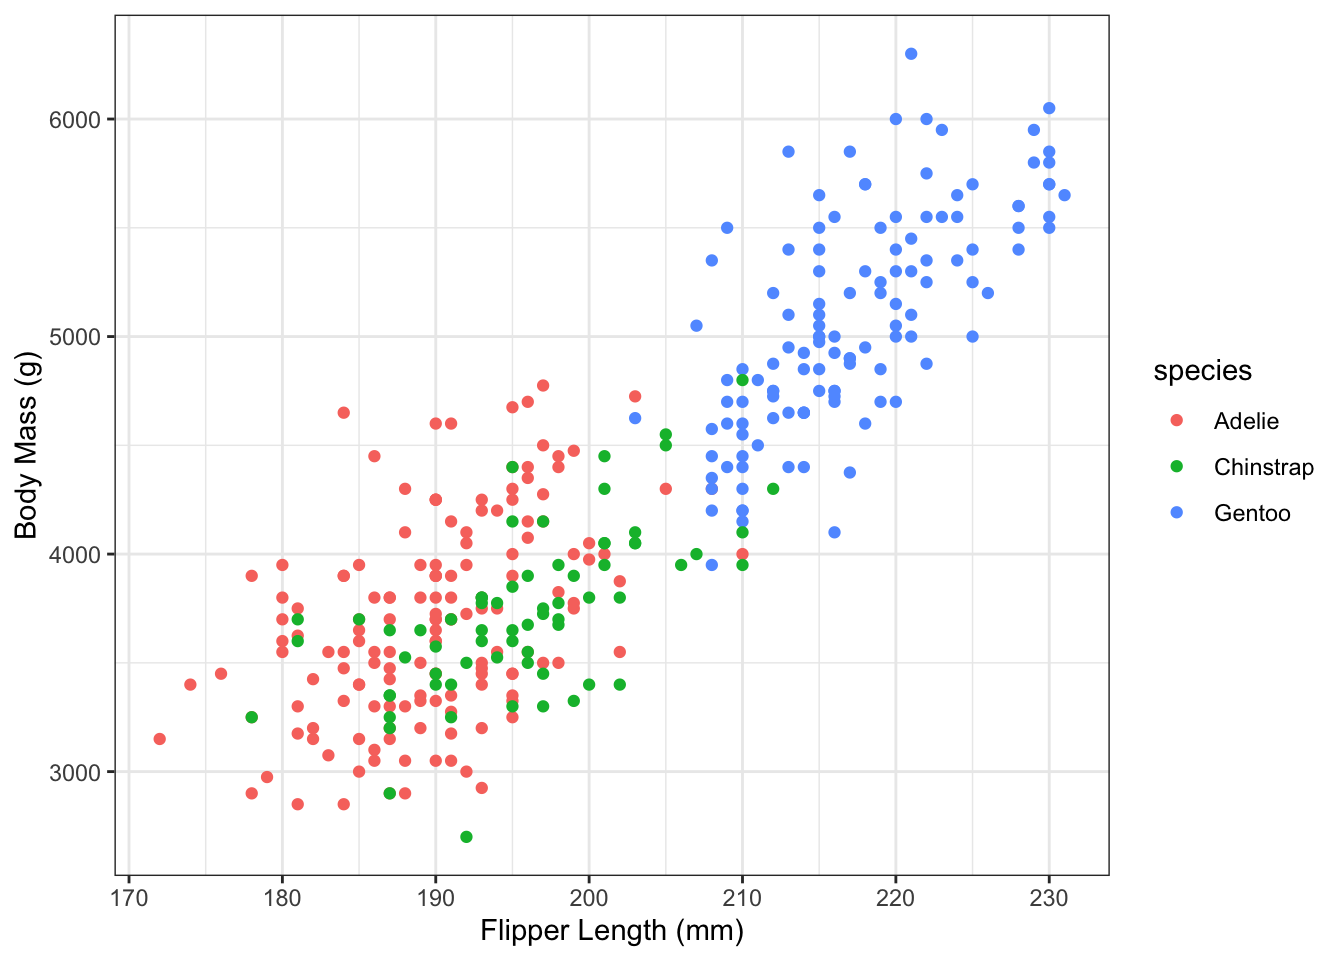
\includegraphics{L03-Scatterplots_Correlation_files/figure-pdf/unnamed-chunk-2-1.pdf}

}

\end{figure}

From this plot, we can see that the three species in these data all have
a similar relationship, but still it might be worth separating out the
groups and seeing what happens!

\hypertarget{the-importance-of-plotting-anscombes-quartet}{%
\section{The Importance of Plotting: Anscombe's
Quartet}\label{the-importance-of-plotting-anscombes-quartet}}

\begin{Shaded}
\begin{Highlighting}[]
\FunctionTok{data.frame}\NormalTok{(}
    \AttributeTok{variable =} \FunctionTok{names}\NormalTok{(anscombe),}
    \AttributeTok{mean =} \FunctionTok{apply}\NormalTok{(anscombe, }\DecValTok{2}\NormalTok{, mean),}
    \AttributeTok{sd =} \FunctionTok{apply}\NormalTok{(anscombe, }\DecValTok{2}\NormalTok{, sd)}
\NormalTok{) }\SpecialCharTok{|\textgreater{}}\NormalTok{ knitr}\SpecialCharTok{::}\FunctionTok{kable}\NormalTok{(}\AttributeTok{row.names =} \ConstantTok{FALSE}\NormalTok{)}
\end{Highlighting}
\end{Shaded}

\begin{longtable}[]{@{}lrr@{}}
\toprule\noalign{}
variable & mean & sd \\
\midrule\noalign{}
\endhead
\bottomrule\noalign{}
\endlastfoot
x1 & 9.000000 & 3.316625 \\
x2 & 9.000000 & 3.316625 \\
x3 & 9.000000 & 3.316625 \\
x4 & 9.000000 & 3.316625 \\
y1 & 7.500909 & 2.031568 \\
y2 & 7.500909 & 2.031657 \\
y3 & 7.500000 & 2.030424 \\
y4 & 7.500909 & 2.030578 \\
\end{longtable}

In this lecture were introducing plots before we talk about numerical
summaries of two variables for a very good reason. The date is it
displayed above is a well-known dataset called Anscombes quartet. Up to
the first two decimal places, all of the variables in the data have the
same mean and standard deviation. If this were all of the information
you had, you might expect the plots to look similar.

\hypertarget{anscombes-quartet}{%
\section{Anscombe's Quartet}\label{anscombes-quartet}}

\begin{Shaded}
\begin{Highlighting}[]
\FunctionTok{par}\NormalTok{(}\AttributeTok{mfrow =} \FunctionTok{c}\NormalTok{(}\DecValTok{2}\NormalTok{,}\DecValTok{2}\NormalTok{), }\AttributeTok{mar =} \FunctionTok{c}\NormalTok{(}\DecValTok{3}\NormalTok{,}\DecValTok{3}\NormalTok{,}\DecValTok{2}\NormalTok{,}\DecValTok{1}\NormalTok{))}
\FunctionTok{plot}\NormalTok{(y1 }\SpecialCharTok{\textasciitilde{}}\NormalTok{ x1, }\AttributeTok{data =}\NormalTok{ anscombe)}
\FunctionTok{abline}\NormalTok{(}\FunctionTok{lm}\NormalTok{(y1 }\SpecialCharTok{\textasciitilde{}}\NormalTok{ x1, }\AttributeTok{data =}\NormalTok{ anscombe))}

\FunctionTok{plot}\NormalTok{(y2 }\SpecialCharTok{\textasciitilde{}}\NormalTok{ x2, }\AttributeTok{data =}\NormalTok{ anscombe)}
\FunctionTok{abline}\NormalTok{(}\FunctionTok{lm}\NormalTok{(y2 }\SpecialCharTok{\textasciitilde{}}\NormalTok{ x2, }\AttributeTok{data =}\NormalTok{ anscombe))}

\FunctionTok{plot}\NormalTok{(y3 }\SpecialCharTok{\textasciitilde{}}\NormalTok{ x3, }\AttributeTok{data =}\NormalTok{ anscombe)}
\FunctionTok{abline}\NormalTok{(}\FunctionTok{lm}\NormalTok{(y3 }\SpecialCharTok{\textasciitilde{}}\NormalTok{ x3, }\AttributeTok{data =}\NormalTok{ anscombe))}

\FunctionTok{plot}\NormalTok{(y4 }\SpecialCharTok{\textasciitilde{}}\NormalTok{ x4, }\AttributeTok{data =}\NormalTok{ anscombe)}
\FunctionTok{abline}\NormalTok{(}\FunctionTok{lm}\NormalTok{(y4 }\SpecialCharTok{\textasciitilde{}}\NormalTok{ x4, }\AttributeTok{data =}\NormalTok{ anscombe))}
\end{Highlighting}
\end{Shaded}

\begin{figure}[H]

{\centering \includegraphics{L03-Scatterplots_Correlation_files/figure-pdf/unnamed-chunk-4-1.pdf}

}

\end{figure}

Clearly, there's a very different pattern in each plot.

\begin{itemize}
\tightlist
\item
  The first plot looks relatively linear with a little bit of random
  variation. For this data set a linear model does seem appropriate.
\item
  The plot at the top right she was a very clear pattern that is not
  linear, so we may be able to fit a model that accounts for this
  non-linearity.
\item
  The plot at the bottom left is almost a perfect line, but with an
  outlier. This outlier makes it so that the line that I have added to
  the plot doesn't actually go through the perfect pattern that we can
  see if that outlier weren't there.
\item
  The bottom right plot is a mess. If it weren't for the outlier, the X
  values would all be identical! In this case, a scatterplot would not
  be appropriate. If I saw this while analysing my data, I would have
  assumed that X was supposed to be either constant (e.g., all X values
  should have been 8) or categorical. In both cases, a scatterplot would
  not be appropriate.
\end{itemize}

Despite all of these wildly different shapes, all of these data sets
have the same summary statistics.

\hypertarget{summarizing-plots}{%
\section{Summarizing Plots}\label{summarizing-plots}}

\begin{itemize}
\tightlist
\item
  Each data point has an \(x\) and a \(y\). We plot \(y\) against \(x\).

  \begin{itemize}
  \tightlist
  \item
    \(y\) is the response, \(x\) is the explanatory variable.\lspace
  \end{itemize}
\item
  We're looking to see if it's linear. Linear models are something we
  know how to deal with!

  \begin{itemize}
  \tightlist
  \item
    Deviations from linearity are noteworthy.
  \item
    Outliers are noteworthy.\lspace
  \end{itemize}
\item
  We can incorporate more information in a scatterplot, especially
  \textbf{categorical variables}.
\end{itemize}

\hypertarget{correlation}{%
\chapter{Correlation}\label{correlation}}

\hypertarget{measuring-strength-of-linearity}{%
\section{Measuring Strength of
Linearity}\label{measuring-strength-of-linearity}}

\vspace{1cm}

From plots, we can sorta see that one looks more linear than another.

\pspace

It would be splendid if we could have a way to quantify this.

\begin{Shaded}
\begin{Highlighting}[]
\FunctionTok{library}\NormalTok{(ggplot2)}
\FunctionTok{theme\_set}\NormalTok{(}\FunctionTok{theme\_bw}\NormalTok{())}
\FunctionTok{library}\NormalTok{(patchwork)}
\NormalTok{x }\OtherTok{\textless{}{-}} \FunctionTok{runif}\NormalTok{(}\DecValTok{100}\NormalTok{, }\DecValTok{0}\NormalTok{, }\DecValTok{10}\NormalTok{)}
\NormalTok{y1 }\OtherTok{\textless{}{-}} \DecValTok{2} \SpecialCharTok{+} \DecValTok{3}\SpecialCharTok{*}\NormalTok{x }\SpecialCharTok{+} \FunctionTok{rnorm}\NormalTok{(}\DecValTok{100}\NormalTok{, }\DecValTok{0}\NormalTok{, }\DecValTok{4}\NormalTok{)}
\NormalTok{y2 }\OtherTok{\textless{}{-}} \DecValTok{2} \SpecialCharTok{+} \DecValTok{3}\SpecialCharTok{*}\NormalTok{x }\SpecialCharTok{+} \FunctionTok{rnorm}\NormalTok{(}\DecValTok{100}\NormalTok{, }\DecValTok{0}\NormalTok{, }\DecValTok{1}\NormalTok{)}

\NormalTok{g1 }\OtherTok{\textless{}{-}} \FunctionTok{ggplot}\NormalTok{() }\SpecialCharTok{+} \FunctionTok{aes}\NormalTok{(}\AttributeTok{x =}\NormalTok{ x, }\AttributeTok{y =}\NormalTok{ y1) }\SpecialCharTok{+} \FunctionTok{geom\_point}\NormalTok{() }\SpecialCharTok{+}
    \FunctionTok{labs}\NormalTok{(}\AttributeTok{title =} \StringTok{"Strong correlation"}\NormalTok{)}
\NormalTok{g2 }\OtherTok{\textless{}{-}} \FunctionTok{ggplot}\NormalTok{() }\SpecialCharTok{+} \FunctionTok{aes}\NormalTok{(}\AttributeTok{x =}\NormalTok{ x, }\AttributeTok{y =}\NormalTok{ y2) }\SpecialCharTok{+} \FunctionTok{geom\_point}\NormalTok{() }\SpecialCharTok{+}
    \FunctionTok{labs}\NormalTok{(}\AttributeTok{title =} \StringTok{"Stronger correlation"}\NormalTok{)}
\NormalTok{g1 }\SpecialCharTok{/}\NormalTok{ g2}
\end{Highlighting}
\end{Shaded}

\begin{figure}[H]

{\centering \includegraphics{L03-Scatterplots_Correlation_files/figure-pdf/unnamed-chunk-5-1.pdf}

}

\end{figure}

From this point on, we're focusing on linear relationships. The plots
above both demonstrate the same linear relationship, but with different
``strength''s. Let's measure that!

\hypertarget{the-correlation-coefficient-r}{%
\section{\texorpdfstring{The correlation coefficient
\(r\)}{The correlation coefficient r}}\label{the-correlation-coefficient-r}}

Recall the formula for the variance: \[
s_x^2 = \frac{1}{n-1}\sum_{i=1}^n(x_i - \bar x)^2 = \frac{1}{n-1}\sum_{i=1}^n(x_i - \bar x)(x_i - \bar x) 
\]

The \textbf{correlation coefficient} is defined as: \[
r = \frac{1}{n-1}\sum_{i=1}^n\left(\frac{x_i - \bar x}{s_x}\right)\left(\frac{y_i - \bar y}{s_y}\right)
\] where \(s_x\) is the s.d. of \(x\) and \(s_y\) is the s.d. of \(y\).

\pspace

It's like a variance for two variables at once!

This explanation might not stick for those of you who aren't a fan of
formulas, but I think this demonstrates an important aspect of the
correlation coefficient. The formula for the standard deviation includes
\((x_i - \bar x)(x_i - \bar x)\). If we replaced one of those with
\(y\), we'd get \((x_i - \bar x)(y_i - \bar y)\), which is one step
closer to the correlation coefficient. In other words, the correlation
is a measure of how two (quantitative) variables vary together!

Let's try another approach. \(x\) has variance. \(y\) has variance. They
also have variance \emph{with each other}. This is measured by the
correlation!

If neither of these explanations make sense, don't worry! We'll see
plenty of correlations and get an intuition for how correlations are
different with different data.

\hypertarget{the-range-of-r}{%
\section{\texorpdfstring{The range of
\(r\)}{The range of r}}\label{the-range-of-r}}

\[
r = \frac{1}{n-1}\sum_{i=1}^n\left(\frac{x_i - \bar x}{s_x}\right)\left(\frac{y_i - \bar y}{s_y}\right)
\]

\begin{itemize}
\tightlist
\item
  \(s_x\) and \(s_y\) are positive\lspace
\item
  \(s_x > \sum_{i=1}^n(x_i - \bar x)\), similar for \(s_y\)

  \begin{itemize}
  \tightlist
  \item
    This can't be larger than 1\lspace
  \end{itemize}
\item
  \(x_i - \bar x\) \emph{can} be negative (same with \((y_i-\bar y)\)).
\end{itemize}

\pspace

The correlation coefficient can be anything from -1 to 1, with 0
representing no correlation and -1 and 1 representing perfect
correlation.

The fact that the correlation can be negative is important. A
correlation coefficient of -1 looks like a perfect downward slope.

\hypertarget{interpreting-correlation}{%
\section{Interpreting correlation}\label{interpreting-correlation}}

\begin{itemize}
\tightlist
\item
  1 and -1 are \textbf{perfect} correlation.\lspace
\item
  0.8 is a strong correlation (depending on context)

  \begin{itemize}
  \tightlist
  \item
    Physics: 0.8 is very very weak.
  \item
    Social science: 0.8 is very very strong.
  \end{itemize}
\end{itemize}

\pspace

\begin{Shaded}
\begin{Highlighting}[]
\NormalTok{shiny}\SpecialCharTok{::}\FunctionTok{runGitHub}\NormalTok{(}\AttributeTok{repo =} \StringTok{"DBecker7/DB7\_TeachingApps"}\NormalTok{, }
    \AttributeTok{subdir =} \StringTok{"Apps/ScatterCorr"}\NormalTok{)}
\end{Highlighting}
\end{Shaded}

The app above shows data that start uncorrelated, then are slowly
transformed into perfect correlation. If you hav R installed on your
computer it should run just fine (you may need to run
\texttt{install.packages("shiny")} for the shiny package, and possibly
\texttt{install.packages("ggplot2")} if you haven't already).

For more examples (and more info on the correlation coefficient in
general), see the
\href{https://www.openintro.org/book/biostat/}{OpenIntro Textbook} and
let me know what you think of that textbook!

\hypertarget{comments-on-the-correlation}{%
\section{Comments on the
correlation}\label{comments-on-the-correlation}}

\[
r = \frac{1}{n-1}\sum_{i=1}^n\left(\frac{x_i - \bar x}{s_x}\right)\left(\frac{y_i - \bar y}{s_y}\right)
\]

\begin{itemize}
\tightlist
\item
  The order of \(x\) and \(y\) can be switched

  \begin{itemize}
  \tightlist
  \item
    2 times 3 is the same as 3 times 2.\lspace
  \end{itemize}
\item
  Since we're subtracting the mean and dividing by the s.d., the units
  don't matter!

  \begin{itemize}
  \tightlist
  \item
    Switching from kg to lbs has no effect on the correlation.\lspace
  \end{itemize}
\item
  \(r>0\) means the line goes up. \(r < 0\) means the line goes
  down.\lspace
\item
  Quantitative only
\item
  Linear only
\item
  \emph{Not} robust to outliers.
\end{itemize}

Let's explore some of these points with code!

\begin{Shaded}
\begin{Highlighting}[]
\FunctionTok{plot}\NormalTok{(y1 }\SpecialCharTok{\textasciitilde{}}\NormalTok{ x1, }\AttributeTok{data =}\NormalTok{ anscombe)}
\end{Highlighting}
\end{Shaded}

\begin{figure}[H]

{\centering \includegraphics{L03-Scatterplots_Correlation_files/figure-pdf/unnamed-chunk-7-1.pdf}

}

\end{figure}

It looks relatively linear. Take a moment to think of how correlated
these two variables are, and assign it a value between 0 and 1. This is
how you would guess the correlation coefficient

On exams, you will be expected to differentiate between ``not
correlated'' (about 0), ``slightly correlated'' (0.2 to 0.4), ``very
correlated'' (0.6 to 0.8), and ``near perfect correlation (almost
exactly 1)'', or the negatives of these values; you won't need to guess
whether the correlation is 0.55 or 0.6.

In R, we calculate the \(r\) with the \texttt{cor()} function.

\begin{Shaded}
\begin{Highlighting}[]
\FunctionTok{cor}\NormalTok{(anscombe}\SpecialCharTok{$}\NormalTok{y1, anscombe}\SpecialCharTok{$}\NormalTok{x1)}
\end{Highlighting}
\end{Shaded}

\begin{verbatim}
[1] 0.8164205
\end{verbatim}

Does this number make sense to you? It seems fairly high to me, but with
small amounts of data it's not that surprising. Think of it this way: if
you removed a quarter of the data at random, would you still be able to
see the pattern? If so, then it's probably ``very correlated''!

The first point states that the order doesn't matter:

\begin{Shaded}
\begin{Highlighting}[]
\FunctionTok{cor}\NormalTok{(anscombe}\SpecialCharTok{$}\NormalTok{y1, anscombe}\SpecialCharTok{$}\NormalTok{x1)}
\end{Highlighting}
\end{Shaded}

\begin{verbatim}
[1] 0.8164205
\end{verbatim}

The units don't matter:

\begin{Shaded}
\begin{Highlighting}[]
\FunctionTok{cor}\NormalTok{(anscombe}\SpecialCharTok{$}\NormalTok{y1}\SpecialCharTok{*}\DecValTok{5} \SpecialCharTok{+} \DecValTok{1}\NormalTok{, anscombe}\SpecialCharTok{$}\NormalTok{x1)}
\end{Highlighting}
\end{Shaded}

\begin{verbatim}
[1] 0.8164205
\end{verbatim}

However, it \emph{does} matter if we do a \emph{non-linear}
transformation, such as squaring the values. The correlation is a
measure of \textbf{linear} association, so making things non-linear will
affect it.

\begin{Shaded}
\begin{Highlighting}[]
\FunctionTok{plot}\NormalTok{(y1}\SpecialCharTok{\^{}}\DecValTok{2} \SpecialCharTok{\textasciitilde{}}\NormalTok{ x1, }\AttributeTok{data =}\NormalTok{ anscombe)}
\end{Highlighting}
\end{Shaded}

\begin{figure}[H]

{\centering \includegraphics{L03-Scatterplots_Correlation_files/figure-pdf/unnamed-chunk-11-1.pdf}

}

\end{figure}

\begin{Shaded}
\begin{Highlighting}[]
\FunctionTok{cor}\NormalTok{(anscombe}\SpecialCharTok{$}\NormalTok{x1, anscombe}\SpecialCharTok{$}\NormalTok{y1}\SpecialCharTok{\^{}}\DecValTok{2}\NormalTok{)}
\end{Highlighting}
\end{Shaded}

\begin{verbatim}
[1] 0.7992029
\end{verbatim}

For these data, squaring didn't have much of an effect (as we can see in
the plot), but we still saw a change in \(r\)! Notice that a unit change
had absolutely no effect on \(r\). In general, we either expect things
to be exactly the same or they can be completely different; very few
things are ``almost equal'' in the general case (they may be almost
equal with one set of data, but that means nothing for completely
different sets of data).

\hypertarget{r-measures-linear-correlation}{%
\section{\texorpdfstring{\(r\) measures \emph{linear}
correlation}{r measures linear correlation}}\label{r-measures-linear-correlation}}

Enzymatic activity is known to be affected by temperature. A study
examined the activity rate (in micromoles per second, μmol/s) of the
digestive enzyme acid phosphatase in vitro at varying temperatures
(measured in kelvins, K). The findings are displayed in the following
table.

\pspace

\begin{enumerate}
\def\labelenumi{\alph{enumi}.}
\tightlist
\item
  Describe the relationship
\item
  Explain why it doesn't make sense to describe this as ``positively
  associated'' or ``negatively associated''.
\item
  Is this a strong or a weak relationship? Explain.
\end{enumerate}

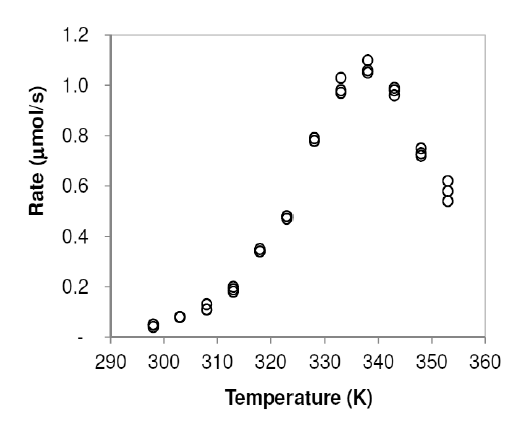
\includegraphics[width=\textwidth]{figs/non-linear.png}

Solutions:

\begin{enumerate}
\def\labelenumi{\alph{enumi}.}
\tightlist
\item
  The relationship increases with an upward curve from temperatures of
  300K to 340K, when it turns downward sharply and decreases to 355K.
\item
  The association is different for different X values. This is
  \emph{not} a linear relationship, which means we have to do extra work
  to make sure that we cover all the non-linearities.
\item
  This is a very strong relationship. The pattern clearly passes the
  facial impact test that we discussed before. It is far from a linear
  relationship, but it's clearly noticable.
\end{enumerate}

\hypertarget{again-always-plot-your-data}{%
\section{Again, always plot your
data!!!}\label{again-always-plot-your-data}}

\vspace{1cm}

All of the plots in the Anscombe quartet \emph{have the same correlation
coefficient}.

\pspace

\(r\) is a measure of linear association - if it's not linear, \(r\)
can't be interpreted!!!

\includegraphics{L03-Scatterplots_Correlation_files/figure-pdf/unnamed-chunk-12-1.pdf}

It's important to note that \(r\) can always be calculated for numeric
data. If we had student numbers as well as a categorical variable that
used 0 to represent black, 1 to represent asian, etc., then we could
technically calculate the correlation coefficient. This would be utterly
meaningless!!!!!

\hypertarget{example-penguins}{%
\section{Example: Penguins}\label{example-penguins}}

\includegraphics{L03-Scatterplots_Correlation_files/figure-pdf/unnamed-chunk-13-1.pdf}

This is an example of something called \textbf{Simpson's Paradox}: If we
don't account for the sub-groups, we get the opposite affect! As we can
see in the plot, if we have all the groups together than it looks like a
negative correlation, but once we separate groups each individual group
has a positive correlation.

(Note that I hid the code for this plot - the code I used to ensure the
colours matched and I got the right layout is pretty advanced, and I
also used some tricks along the way.)

\hypertarget{correlation-summary}{%
\section{Correlation Summary}\label{correlation-summary}}

\begin{itemize}
\tightlist
\item
  \(r\) is a measure of \textbf{linear} association

  \begin{itemize}
  \tightlist
  \item
    I've said it plenty, I'll say it again: \(r\) does not apply to
    non-linear patterns!
  \item
    Always plot your data before calculating \(r\).\lspace
  \end{itemize}
\item
  \(r\) is like a measure of how two variables vary together.

  \begin{itemize}
  \tightlist
  \item
    Formula is similar to the variance formula!\lspace
  \end{itemize}
\item
  \(r\) is a number between -1 and 1, with 0 meaning no correlation and
  1 or -1 meaning perfect correlation.

  \begin{itemize}
  \tightlist
  \item
    A negative \(r\) means a negative relationship (i.e.~a line that
    goes down).\lspace
  \end{itemize}
\item
  Everything on the ``Comments'' slide is fair game for test questions.
\end{itemize}

\hypertarget{participation-questions}{%
\chapter{Participation Questions}\label{participation-questions}}

\hypertarget{q01}{%
\section{Q01}\label{q01}}

The correlation coefficient measures the strength of the correlation.

\begin{enumerate}
\def\labelenumi{\arabic{enumi}.}
\tightlist
\item
  True
\item
  False
\end{enumerate}

\hypertarget{q02}{%
\section{Q02}\label{q02}}

If \(r < 0\), there is a negative linear correlation.

\begin{enumerate}
\def\labelenumi{\arabic{enumi}.}
\tightlist
\item
  True
\item
  False
\end{enumerate}

\hypertarget{q03}{%
\section{Q03}\label{q03}}

Which of the following represents the \emph{strongest} correlation?

\begin{enumerate}
\def\labelenumi{\arabic{enumi}.}
\tightlist
\item
  0.4
\item
  0.7
\item
  -0.8
\item
  0
\end{enumerate}

\hypertarget{q04}{%
\section{Q04}\label{q04}}

\vspace{1cm}

What is the best description of the plot on the right?

\begin{enumerate}
\def\labelenumi{\arabic{enumi}.}
\tightlist
\item
  No correlation, has an outlier.
\item
  Strong correlation, has an outlier
\item
  Slight negative correlation
\item
  Shapeless
\end{enumerate}

\begin{Shaded}
\begin{Highlighting}[]
\NormalTok{x }\OtherTok{\textless{}{-}} \FunctionTok{c}\NormalTok{(}\FunctionTok{runif}\NormalTok{(}\DecValTok{99}\NormalTok{, }\DecValTok{0}\NormalTok{, }\DecValTok{10}\NormalTok{), }\DecValTok{11}\NormalTok{)}
\NormalTok{y }\OtherTok{\textless{}{-}} \FunctionTok{c}\NormalTok{(}\FunctionTok{rnorm}\NormalTok{(}\DecValTok{99}\NormalTok{), }\DecValTok{20}\NormalTok{)}

\FunctionTok{ggplot}\NormalTok{() }\SpecialCharTok{+} \FunctionTok{aes}\NormalTok{(}\AttributeTok{x =}\NormalTok{ x, }\AttributeTok{y =}\NormalTok{ y) }\SpecialCharTok{+} \FunctionTok{geom\_point}\NormalTok{() }\CommentTok{\#+ }
\end{Highlighting}
\end{Shaded}

\begin{figure}[H]

{\centering \includegraphics{L03-Scatterplots_Correlation_files/figure-pdf/unnamed-chunk-14-1.pdf}

}

\end{figure}

\begin{Shaded}
\begin{Highlighting}[]
    \CommentTok{\#geom\_smooth(method = "lm", formula = y\textasciitilde{}x, se = FALSE)}
\end{Highlighting}
\end{Shaded}

\hypertarget{extra-context-fitting-a-line}{%
\section{Extra context: Fitting a
Line}\label{extra-context-fitting-a-line}}

\vspace{1cm}

A line would try and fit the outlier, which misleads us into thinking
there might be a correlation!

\begin{Shaded}
\begin{Highlighting}[]
\FunctionTok{ggplot}\NormalTok{() }\SpecialCharTok{+} \FunctionTok{aes}\NormalTok{(}\AttributeTok{x =}\NormalTok{ x, }\AttributeTok{y =}\NormalTok{ y) }\SpecialCharTok{+} \FunctionTok{geom\_point}\NormalTok{() }\SpecialCharTok{+} 
    \FunctionTok{geom\_smooth}\NormalTok{(}\AttributeTok{method =} \StringTok{"lm"}\NormalTok{, }\AttributeTok{formula =}\NormalTok{ y}\SpecialCharTok{\textasciitilde{}}\NormalTok{x, }\AttributeTok{se =} \ConstantTok{FALSE}\NormalTok{)}
\end{Highlighting}
\end{Shaded}

\begin{figure}[H]

{\centering \includegraphics{L03-Scatterplots_Correlation_files/figure-pdf/unnamed-chunk-15-1.pdf}

}

\end{figure}

\hypertarget{q05}{%
\section{Q05}\label{q05}}

Which statement is \emph{true}.

\begin{enumerate}
\def\labelenumi{\arabic{enumi}.}
\tightlist
\item
  The explanatory variable causes the response.
\item
  The response must be something measured \emph{after} the explanatory
  variable.
\item
  We use the explanatory variable to explain the response, without
  assuming causality.
\item
  The correlation between the explanatory and response variable will be
  positive if the explanatory causes the response, negative if the
  response causes the explanatory.
\end{enumerate}

\hypertarget{q06}{%
\section{Q06}\label{q06}}

We can add colour to a plot using what type of variable?

\begin{enumerate}
\def\labelenumi{\arabic{enumi}.}
\tightlist
\item
  Categorical
\item
  Quantitative
\end{enumerate}

\textbf{Exercises:}

\begin{enumerate}
\def\labelenumi{\arabic{enumi}.}
\tightlist
\item
  The following code will draw a plot and calculate the correlation
  coefficient. Currently, it's doing this for the column \texttt{mpg}
  (response) versus the column \texttt{wt} (``weight'', explanatory) in
  the \texttt{mtcars} data which is built in to R.

  \begin{enumerate}
  \def\labelenumii{\alph{enumii}.}
  \tightlist
  \item
    Re-run the code, but replace \texttt{wt} with \texttt{disp} (engine
    displacement), \texttt{hp} (horsepower), \texttt{drat} (rear axle
    ratio, although I couldn't explain this further), and \texttt{qsec}
    (quarter mile time, in seconds). Comment on the apparent pattern and
    the magnitude of the correlation.
  \item
    Change \texttt{wt} to\texttt{cyl}, the number of cylinders. What do
    you notice about the plot, and how does this affect your
    interpretation of the correlation between \texttt{mpg} and
    \texttt{cyl}? Explain why \texttt{cyl} might be better incorporated
    as a categorical variable, even though it is indeed numeric.
  \item
    Repeat part (b) for \texttt{am}, which is ``0'' for automatic
    transmission and ``1'' for manual transmission.
  \end{enumerate}
\end{enumerate}

\begin{Shaded}
\begin{Highlighting}[]
\FunctionTok{plot}\NormalTok{(mpg }\SpecialCharTok{\textasciitilde{}}\NormalTok{ wt, }\AttributeTok{data =}\NormalTok{ mtcars)}
\end{Highlighting}
\end{Shaded}

\begin{figure}[H]

{\centering \includegraphics{L03-Scatterplots_Correlation_files/figure-pdf/unnamed-chunk-16-1.pdf}

}

\end{figure}

\begin{Shaded}
\begin{Highlighting}[]
\FunctionTok{cor}\NormalTok{(mtcars}\SpecialCharTok{$}\NormalTok{mpg, mtcars}\SpecialCharTok{$}\NormalTok{wt)}
\end{Highlighting}
\end{Shaded}

\begin{verbatim}
[1] -0.8676594
\end{verbatim}

\begin{enumerate}
\def\labelenumi{\arabic{enumi}.}
\setcounter{enumi}{1}
\tightlist
\item
  The following figure comes from the article ``Shared neural
  representations and temporal segmentation of political content predict
  ideological similarity'' by De Brujin et al., published in 2023
  (\href{https://www.science.org/doi/10.1126/sciadv.abq5920}{link to
  aricle here}). The star on the plot indicates that they have found a
  statistically significant relationship (more on this next week). Is
  this a strong correlation?
\end{enumerate}

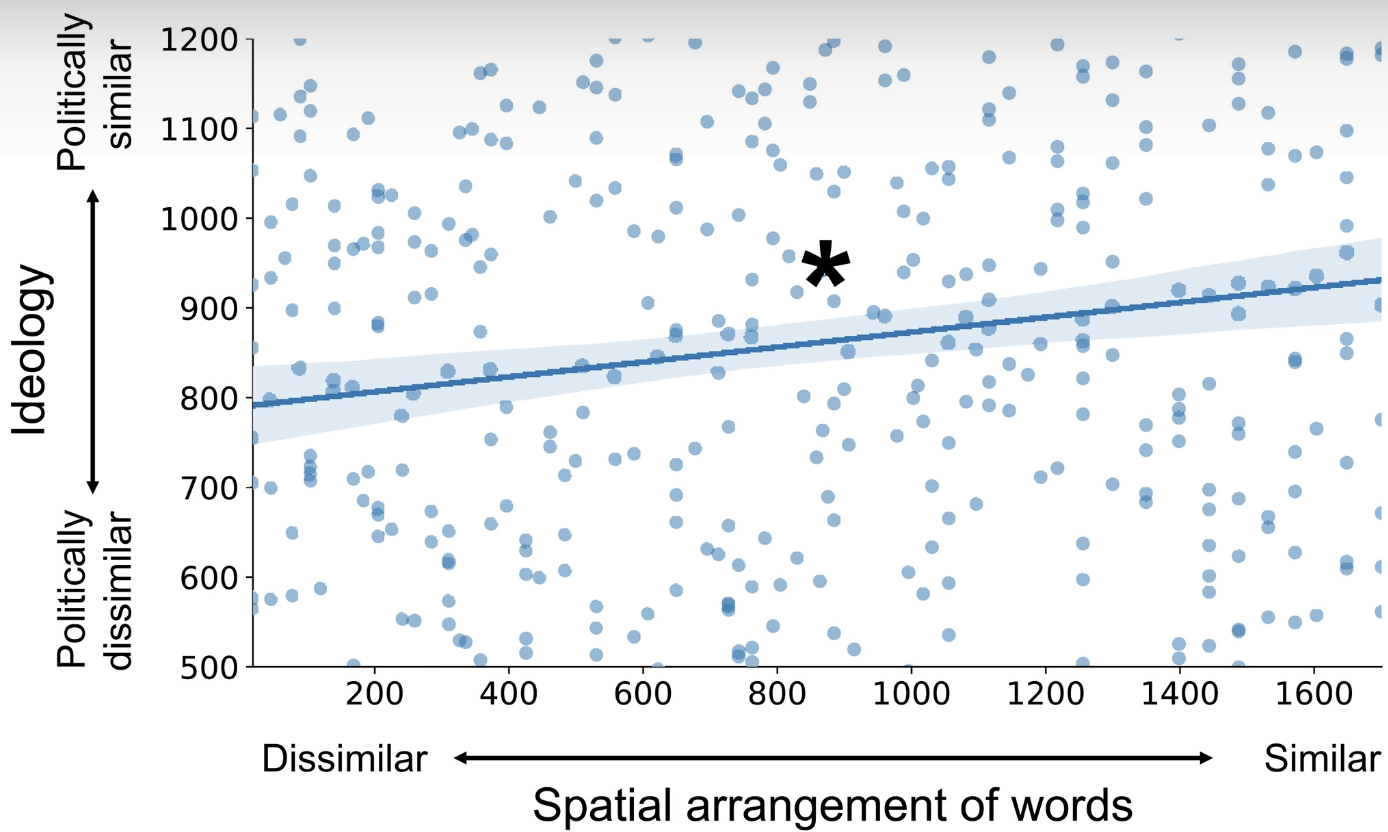
\includegraphics[width=0.7\textwidth]{figs/scatterbad.png}

\begin{enumerate}
\def\labelenumi{\arabic{enumi}.}
\setcounter{enumi}{2}
\tightlist
\item
  The following figure comes from the article ``Effect on Blood Pressure
  of Daily Lemon Ingestion and Walking'' by Kato et al., published in
  2013 (\href{https://www.hindawi.com/journals/jnme/2014/912684/}{link
  to article here}). Comment on the shape of this relationship. Recall
  how we described a ``strong'' shape as a shape that remains even if
  some of the data points were removed.
\end{enumerate}

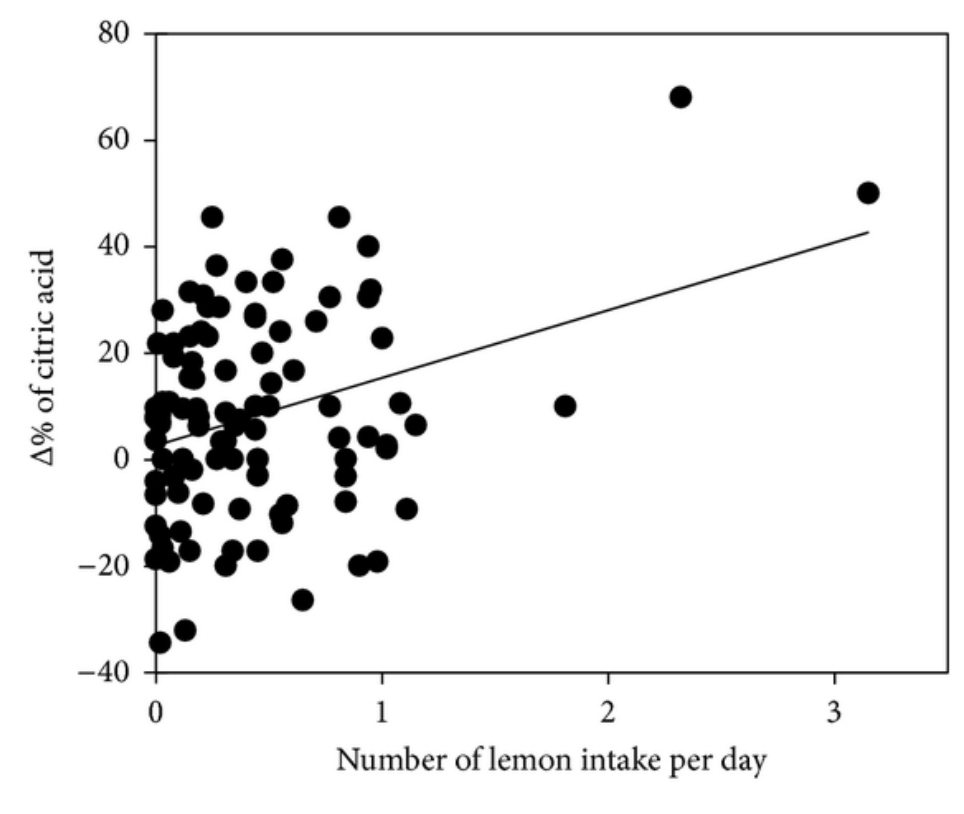
\includegraphics[width=0.5\textwidth]{figs/lemon.png}

\textbf{Exercises from Baldi \& Moore textbook}

\begin{enumerate}
\def\labelenumi{\arabic{enumi}.}
\setcounter{enumi}{3}
\tightlist
\item
  (3.13) You have data for many individuals on their walking speed and
  their heart rate after a 10-minute walk. When you make a scatterplot,
  the explanatory variable on the x axis

  \begin{enumerate}
  \def\labelenumii{\alph{enumii}.}
  \tightlist
  \item
    is walking speed.
  \item
    is heart rate.
  \item
    doesn't matter.
  \end{enumerate}
\item
  (3.18) If mothers were always 2 years younger than the fathers of
  their children, the correlation between the ages of mother and father
  would be

  \begin{enumerate}
  \def\labelenumii{\alph{enumii}.}
  \item
    \begin{enumerate}
    \def\labelenumiii{\arabic{enumiii}.}
    \tightlist
    \item
    \end{enumerate}
  \item
    0.5.
  \item
    Can't tell without seeing the data.
  \end{enumerate}
\item
  (3.19) For a class project, you measure the weight in grams and the
  tail length in millimeters of a group of mice. The correlation is
  \(r = 0.7\). The scatterplot shows one outlier of the relationship,
  falling clearly below the overall pattern of points. It turns out that
  this mouse was sick, and you decide to exclude it from the data set.
  With the outlier removed, you can expect the value of \(r\) to:

  \begin{enumerate}
  \def\labelenumii{\alph{enumii}.}
  \tightlist
  \item
    stay the same.
  \item
    increase.
  \item
    decrease.
  \end{enumerate}
\end{enumerate}

\textbf{Exercises from OpenIntro Biotatistics textbook}

Questions 1.35, 1.36, 1.37.

For further R practice and case studies, see the
\href{https://www.openintro.org/book/statlabs/?labblock=biostat_intro_to_data}{labs
page for the OpenIntro textbook}.

\hypertarget{regression}{%
\chapter{Regression}\label{regression}}

\hypertarget{preamble-2}{%
\chapter{Preamble}\label{preamble-2}}

\hypertarget{announcements-3}{%
\section{Announcements}\label{announcements-3}}

\hypertarget{agenda-3}{%
\section{Agenda}\label{agenda-3}}

\hypertarget{introduction-1}{%
\chapter{Introduction}\label{introduction-1}}

These notes are based on Chapter 4 of Baldi \& Moore and Chapter 6.1 to
6.3 in OpenIntro Biostats.

In linear modelling, we have a collection of pairs \(x_i\) and \(y_i\).
We think that there's some sort of relationship between \(x\) and \(y\),
and we think that a line is an adequate way to characterize that
relationship\footnote{Very few things are actually linear, but lines are
  fantastic approximations to many things.}.

Just like we assume that there's a ``true'' population mean, there is
also a ``true'' slope and intercept for the line that characterizes the
relationship between \(x\) and \(y\). In the plot below, the green line
represents the ``true'' relationship between \(x\) and \(y\), and the
data are random values above and below that line\footnote{We assume that
  \(x\) is fixed, but \(y\) has random noise. In other words, \(x\) is
  not a random variable but \(y\) is.}.

\includegraphics{L04-Regression_files/figure-pdf/unnamed-chunk-1-1.pdf}

In high school, you may have learned a line as \(y = mx + b\). In
statistics, we often use latin letters for estimates and greek letters
for population parameters\footnote{Because we think it makes us fancy.
  Note that the Baldi \& Moore textbook uses \(a\), \(b\), and \(e\) for
  everything.}. The population line is thus:

\[
y_i = \alpha + \beta x_i + \epsilon_i
\]

\begin{itemize}
\tightlist
\item
  \(\alpha\) is the \textbf{intercept}.
\item
  \(\beta\) is the \textbf{slope}.

  \begin{itemize}
  \tightlist
  \item
    A 1 unit increase in \(x\) corresponds to a \(\beta\) increase in
    \(y\).
  \end{itemize}
\item
  \(\epsilon_i\) is random noise (\(N(0,\sigma)\)).

  \begin{itemize}
  \tightlist
  \item
    Again, we think of \(x\) as being fixed. The random noise is above
    and below the line, not side to side.
  \end{itemize}
\item
  The formula implies that \(y_i \sim N(\alpha + \beta x_i, \sigma)\),
  since \(y_i\) is centered at \(\alpha + \beta x_i\) but randomly
  varies above and below the line with variance \(\sigma^2\).
\end{itemize}

The word ``regression'' means to go backward. I like to think that we
are ``going backward'' to the population numbers from the sample
values\footnote{Actually, the word comes from ``regressing to the
  mean'', which comes from how children are closer to average height
  than their parents - they go back toward the mean. This is not
  important.}. Any situation where you are estimating a population
parameter is technically a \textbf{regression}, but this terminology is
not useful for this class.

To regress, we \textbf{estimate} the parameters using sample statistics.
For linear regression, we use regular old latin letters instead of the
fancy greek ones. \(a\) is the estimate for \(\alpha\), \(b\) for
\(\beta\), and \(e\) for \(\epsilon\). In order to do find these sample
statistics, we minimize the squared error between the line and the data:

\[e_i^2 = (y_i - a - b x_i)^2\]

In other words, we find \(a\) (for \(\alpha\)) and \(b\) (for \(\beta\))
that make the sum of the squared errors \(e_i\) as small as possible. We
use the squared errors for the same reason we use squared deviations in
the forumla for the variance: so that positive and negative values do
not cancel out\footnote{Also, because the calculus works out so much
  better.}.

The estimates \(a\) and \(b\) are as follows:

\begin{align*}
b &= rs_y/s_x\\
a &= \bar y - b\bar x
\end{align*}

These are called the \textbf{least squares} estimates\footnote{There are
  other ways to estimate these parameters, but they're outside the scope
  of this course. All regression lines that you see in the textbook and
  the notes will be least squares regression lines.}. The equation for
\(b\) is especially important!

In R, these can be calculated as follows. The \texttt{mtcars} data set
is a collection of measurements made on various cars. In this example,
we'll regress the fuel efficiency (in miles per gallon, or mpg) against
the weight of the car.

\begin{Shaded}
\begin{Highlighting}[]
\CommentTok{\# Load a built{-}in data set}
\FunctionTok{data}\NormalTok{(mtcars) }

\CommentTok{\# Define which variables are x and y.}
\CommentTok{\# This isn\textquotesingle{}t necessary, but helps with teaching}
\NormalTok{x }\OtherTok{\textless{}{-}}\NormalTok{ mtcars}\SpecialCharTok{$}\NormalTok{wt}
\NormalTok{y }\OtherTok{\textless{}{-}}\NormalTok{ mtcars}\SpecialCharTok{$}\NormalTok{mpg}

\CommentTok{\# Calculate the estimates by hand}
\NormalTok{b }\OtherTok{\textless{}{-}} \FunctionTok{cor}\NormalTok{(x, y) }\SpecialCharTok{*} \FunctionTok{sd}\NormalTok{(y) }\SpecialCharTok{/} \FunctionTok{sd}\NormalTok{(x)}
\NormalTok{a }\OtherTok{\textless{}{-}} \FunctionTok{mean}\NormalTok{(y) }\SpecialCharTok{{-}}\NormalTok{ b }\SpecialCharTok{*} \FunctionTok{mean}\NormalTok{(x)}

\CommentTok{\# Print the estimates }
\FunctionTok{c}\NormalTok{(a, b)}
\end{Highlighting}
\end{Shaded}

\begin{verbatim}
[1] 37.285126 -5.344472
\end{verbatim}

\begin{Shaded}
\begin{Highlighting}[]
\CommentTok{\# Use the built{-}in functions}
\FunctionTok{summary}\NormalTok{(}\FunctionTok{lm}\NormalTok{(y }\SpecialCharTok{\textasciitilde{}}\NormalTok{ x))}
\end{Highlighting}
\end{Shaded}

\begin{verbatim}

Call:
lm(formula = y ~ x)

Residuals:
    Min      1Q  Median      3Q     Max 
-4.5432 -2.3647 -0.1252  1.4096  6.8727 

Coefficients:
            Estimate Std. Error t value Pr(>|t|)    
(Intercept)  37.2851     1.8776  19.858  < 2e-16 ***
x            -5.3445     0.5591  -9.559 1.29e-10 ***
---
Signif. codes:  0 '***' 0.001 '**' 0.01 '*' 0.05 '.' 0.1 ' ' 1

Residual standard error: 3.046 on 30 degrees of freedom
Multiple R-squared:  0.7528,    Adjusted R-squared:  0.7446 
F-statistic: 91.38 on 1 and 30 DF,  p-value: 1.294e-10
\end{verbatim}

From this line, we can make \textbf{predictions} about new points by
simply plugging in the \(x\) value. For example, let's say we wanted to
guess the mpg of a car that weighs 3,000 lbs. In the data, the units for
weight are 1000 lbs, so this means plugging a value of \texttt{wt=3}
into the data.

\begin{Shaded}
\begin{Highlighting}[]
\NormalTok{a }\SpecialCharTok{+}\NormalTok{ b}\SpecialCharTok{*}\DecValTok{3}
\end{Highlighting}
\end{Shaded}

\begin{verbatim}
[1] 21.25171
\end{verbatim}

So we would guess that a 3 ton car would have a fuel efficiency of 21.25
miles per gallon. Let's look at this on a plot:

\begin{Shaded}
\begin{Highlighting}[]
\FunctionTok{plot}\NormalTok{(y }\SpecialCharTok{\textasciitilde{}}\NormalTok{ x)}
\FunctionTok{points}\NormalTok{(}\DecValTok{3}\NormalTok{, a }\SpecialCharTok{+}\NormalTok{ b}\SpecialCharTok{*}\DecValTok{3}\NormalTok{, }\AttributeTok{col =} \StringTok{"red"}\NormalTok{, }\AttributeTok{pch =} \DecValTok{16}\NormalTok{)}
\end{Highlighting}
\end{Shaded}

\begin{figure}[H]

{\centering \includegraphics{L04-Regression_files/figure-pdf/unnamed-chunk-4-1.pdf}

}

\end{figure}

It looks like this is somewhere around where we would expect.

If we repeat this for every possible \(x\) value, we get the regression
line below:

\begin{Shaded}
\begin{Highlighting}[]
\FunctionTok{plot}\NormalTok{(y }\SpecialCharTok{\textasciitilde{}}\NormalTok{ x)}
\FunctionTok{points}\NormalTok{(}\DecValTok{3}\NormalTok{, a }\SpecialCharTok{+}\NormalTok{ b}\SpecialCharTok{*}\DecValTok{3}\NormalTok{, }\AttributeTok{col =} \StringTok{"red"}\NormalTok{, }\AttributeTok{pch =} \DecValTok{16}\NormalTok{)}
\CommentTok{\# abline adds a line with slope b and intercept a to a plot.}
\FunctionTok{abline}\NormalTok{(}\AttributeTok{a =}\NormalTok{ a, }\AttributeTok{b =}\NormalTok{ b, }\AttributeTok{col =} \StringTok{"red"}\NormalTok{)}
\end{Highlighting}
\end{Shaded}

\begin{figure}[H]

{\centering \includegraphics{L04-Regression_files/figure-pdf/unnamed-chunk-5-1.pdf}

}

\end{figure}

We cal also see the values of \(e\), the residuals.

\begin{Shaded}
\begin{Highlighting}[]
\NormalTok{e }\OtherTok{\textless{}{-}}\NormalTok{ y }\SpecialCharTok{{-}}\NormalTok{ (a }\SpecialCharTok{+}\NormalTok{ b}\SpecialCharTok{*}\NormalTok{x)}
\FunctionTok{plot}\NormalTok{(e }\SpecialCharTok{\textasciitilde{}}\NormalTok{ x, }\AttributeTok{main =} \StringTok{"Plot of the Residuals"}\NormalTok{)}
\CommentTok{\# abline can also draw a line with slope 0 (horizontal)}
\FunctionTok{abline}\NormalTok{(}\AttributeTok{h =} \DecValTok{0}\NormalTok{, }\AttributeTok{col =} \StringTok{"grey"}\NormalTok{)}
\end{Highlighting}
\end{Shaded}

\begin{figure}[H]

{\centering \includegraphics{L04-Regression_files/figure-pdf/unnamed-chunk-6-1.pdf}

}

\end{figure}

\hypertarget{regression-facts}{%
\chapter{Regression Facts}\label{regression-facts}}

Here are some facts about the least squares regression line:

\begin{itemize}
\tightlist
\item
  The point \((\bar x, \bar y)\) is always on the line.

  \begin{itemize}
  \tightlist
  \item
    Least squares regression can be seen as putting a line through
    \((\bar x, \bar y)\) and rotating it until the squared error is the
    smallest.
  \end{itemize}
\item
  \(s_y\ge 0\) and \(s_x\ge 0\), so whenever \(r > 0\), we know that
  \(b > 0\).

  \begin{itemize}
  \tightlist
  \item
    The slope has the same sign as the correlation. Otherwise, the slope
    could be pretty much any number, regardless of the correlation.
  \item
    If \(r = 0\), then \(b = 0\), and vice versa.
  \item
    Other than the sign and the special case of \(r=0\), there is no way
    to tell the value of \(r\) if all you know is \(b\).
  \end{itemize}
\item
  For \(r\), the distinction between \(y\) and \(x\) doesn't matter.

  \begin{itemize}
  \tightlist
  \item
    For the regression line, it \emph{absolutely} matters!
  \end{itemize}
\item
  The sum of the errors is 0.
\end{itemize}

\begin{Shaded}
\begin{Highlighting}[]
\CommentTok{\# The prediction at mean(x) is equal to mean(y)}
\CommentTok{\# In other words, (mean(x), mean(y)) is a point on the line}
\NormalTok{a }\SpecialCharTok{+}\NormalTok{ b }\SpecialCharTok{*} \FunctionTok{mean}\NormalTok{(x)}
\end{Highlighting}
\end{Shaded}

\begin{verbatim}
[1] 20.09062
\end{verbatim}

\begin{Shaded}
\begin{Highlighting}[]
\FunctionTok{mean}\NormalTok{(y)}
\end{Highlighting}
\end{Shaded}

\begin{verbatim}
[1] 20.09062
\end{verbatim}

\begin{Shaded}
\begin{Highlighting}[]
\CommentTok{\# Correlation doesn\textquotesingle{}t care about order}
\FunctionTok{cor}\NormalTok{(x, y)}
\end{Highlighting}
\end{Shaded}

\begin{verbatim}
[1] -0.8676594
\end{verbatim}

\begin{Shaded}
\begin{Highlighting}[]
\FunctionTok{cor}\NormalTok{(y, x)}
\end{Highlighting}
\end{Shaded}

\begin{verbatim}
[1] -0.8676594
\end{verbatim}

\begin{Shaded}
\begin{Highlighting}[]
\CommentTok{\# Theoretically 0, but computers aren\textquotesingle{}t perfectly precise}
\CommentTok{\# Note: e{-}14 refers to 10\^{}{-}14, or 14 zeroes before the first digit}
    \CommentTok{\# So, pretty close to 0.}
\FunctionTok{sum}\NormalTok{(e) }
\end{Highlighting}
\end{Shaded}

\begin{verbatim}
[1] 1.065814e-14
\end{verbatim}

\hypertarget{percent-of-variation-explained}{%
\chapter{Percent of Variation
Explained}\label{percent-of-variation-explained}}

Because of some mathematical quirks, \(r^2\), the squared value of
\(r\), can be interpreted as:

\begin{quote}
\textbf{The percent of variation in \(y\) that can be ``explained'' by
the linear model}.\footnote{Usually \(r^2\) is labelled \(R^2\) for
  historical reasons. Capitalization matters in math; it's just
  coincidence that both lower case and upper case mean the same thing
  here.}
\end{quote}

The value of \(r^2\) can be calculated as: \[
R^2 = r^2 = \frac{\text{Variance of the predicted }y\text{-values}}{\text{Variance of the observed }y\text{-values}}
\]

I'll explain this in steps. The first plot below shows just the values
in \(y\). This collection of values has a own mean and variance.

The second plot shows the change in variance that the line ``explains''.
Instead of deviations above and below the mean, the variance can now be
characterized as the deviations above and below the regression line.
This variance will always be lower than the variance of \(y\) without
incorporating \(x\)\footnote{Except when \(r=0\), can you explain why?}.

The third plot shows where this variance went. \emph{The line itself has
variance}; there is deviation in the line above and below the mean of
\(y\). This is the variance that gets explained by incorporating \(x\)!
If you consider one of the points in \(y\), say \(y_1\), the distance
between \(y_1\) and \(\bar y\) can be split up into the difference
between \(\bar y\) and the regression line plus the distance between the
regression line and \(y_1\).

\includegraphics{L04-Regression_files/figure-pdf/unnamed-chunk-8-1.pdf}

The rest of the variance is left \textbf{unexplianed}. No regression
will ever be perfect unless we are studing a very very simple .

To see this a different way, consider what happens when
\(r = 0\)\footnote{Therefore the slope will also be 0.}. This will just
be a horizontal line, and none of the variance is explained. On the
other had, if \(r = 1\) then all of the points will be exactly on the
line. All of the variance in \(y\) has been explained by the regression
against \(x\) - there's no variance left to be explained!\footnote{Statistics
  is \emph{still} just the study of variance.}

Notice how the R output includes

\hypertarget{extensions-and-cautions}{%
\chapter{Extensions and Cautions}\label{extensions-and-cautions}}

\hypertarget{prediction}{%
\section{Prediction}\label{prediction}}

For a new \(x\) value, \[y = a + bx\] is the \textbf{predicted} value of
\(y\). That is, if we have an \(x\) value, we can plug it into the
equation and find out what value of \(y\) we would expect.

Note: There is still variance around this prediction! Our ``expected''
value will never be exactly equal to the truth - The value of \(y\) at a
given value of \(x\) follows a normal distribution\footnote{Our
  \textbf{prediction} is just us guessing the mean value of \(y\) at
  different values of \(x\).}, and the probability of a single point is
0!

\hypertarget{extrapolation}{%
\section{Extrapolation}\label{extrapolation}}

\textbf{Extrapolation} is what happens when prediction goes wrong. In
particular, it's what happens when we try to make a prediction at an
\(x\) value where we don't have any data. Usually this means we're
predicting an \(x\) value far above or far below the range of our data,
but it can also happen if there's a gap in the middle of our data.

In the plot below, the black dots are the original data, and we're
trying to predict a new value at \(x = 25\). The red line is the true
model that I generated the data from. The black line represents a linear
model. This model fits the original data quite well\footnote{Even though
  it's not the true relationship, it's a reasonable approximation.}, but
predictions are completely inappropriate for values outside the data.

\includegraphics{L04-Regression_files/figure-pdf/unnamed-chunk-9-1.pdf}

\hypertarget{lurking-variables}{%
\section{Lurking Variables}\label{lurking-variables}}

The black line in the plot below represents a regression where all of
the data was lumped together. As we can see, this line does not seem to
fit the data well. There is a hidden relationship in the the data - the
green points and the red points should be considered
separately\footnote{Possibly as a blocking variable.}.

\includegraphics{L04-Regression_files/figure-pdf/unnamed-chunk-10-1.pdf}

A more serious consequence of a lurking variable has shown up before in
the Palmer penguins data. In that example, the lurking variable actually
\textbf{reversed} the correlation - if we lumped the groups together we
got a negative correlation (and therefore negative slope), but if we
looked at the groups individually we got positive associations in all of
the groups! This is called \textbf{Simpson's Paradox}, and basically
means that we have to be very careful about interpreting correlations!

\includegraphics{L04-Regression_files/figure-pdf/unnamed-chunk-11-1.pdf}

\hypertarget{probability-background}{%
\chapter{Probability Background}\label{probability-background}}

Please pay attention to the margin notes.\footnote{These things!} They
often contain important information.\footnote{Or silliness.}

These notes are based on Chapter 9 in Baldi \& Moore (4th edition).
Chapter 2 of \href{https://www.openintro.org/book/biostat}{OpenIntro
Biostatics} is also a great (free) resource.

\hypertarget{defining-probability-with-dice}{%
\chapter{Defining Probability with
Dice}\label{defining-probability-with-dice}}

I find that the easiest way is to build this up by examples. Let's start
with rolling a dice.\footnote{The singular form ``die'' is dieing out;
  the dictionary lists ``dice'' as singular noun, and the singular
  ``dice'' is clearer for new English speakers.} Let's say you rolled
the dice, and you got a 3. This is called a \textbf{simple event}. The
collection of all \textbf{simple events} is called the \textbf{Sample
Space}, which in this case is \(\mathcal S\)=\{1,2,3,4,5,6\}.

Now, suppose that you're about to roll a dice. You might be curious
about whether it's a 1, 2, 3, 4, 5, or a 6, but you might only care
about the \textbf{event} that the outcome is even. Since there are
multiple simple events that make up this event, it is called a
\textbf{compound event}.

There's no way for you to know what's going to happen, but you know all
of the possibilities and you know how likely they all are.\footnote{Assuming
  there's nothing unusual about your dice.} This is called a
\textbf{Probability Model}: The sample space along with the probability
of all of the events.

I said ``the probability of all events'', but this is more complicated
than it may seem and requires some explanation. For something like
rolling a dice, you only need to know the probability of each simple
event. Compound events, like the probability that the outcome is even,
can be determined from these simple events.

Suppose you're playing a game where, if the outcome of the dice is less
than a certain cutoff value you get to roll again (e.g., your character
has a special ability that allows re-rolling of dice, but the re-roll
condition depends on the situation). You know the probability of all of
the simple events, but you need to know the cutoff value to actually
compute any probabilities. Without the cutoff value, you cannot define
the probability model.

For a dice, the probability model is simply: Each number has a
probability of 1 in 6. But what does this mean? There are two
perspectives on what a ``probability'' is: The Frequentist approach and
the Bayesian approach. In this class we're only going to learn the
Frequentist definition of probability, but if you're interested in
learning more I'm happy to talk.\footnote{Most of my work uses the
  Bayesian definition.}

\textbf{Probability} (Frequentist Definition): The long run frequency of
observing an event. In other words, it's the number of times an event is
observed divided by the number of trials after doing a near-infinite
number of trials.

For the dice, if we rolled the dice 60 times, we would expect 10 of
those rolls to be a 1, 10 of them to be a 2, etc. Due to randomness, we
won't get exactly that, but this is what we would expect. If we rolled
600 dice, we would expect 100 to be 1, etc. As we roll more dice, we get
closer to the proportion of 1/6. The plot below this demonstrates this -
it is the number of times that a dice was 1 divided by the number of
trials, with the number of trials being increased. Notice how it takes a
while for the ``empirical'' probability to reach the theoretical
probably; as the number of trials approaches infinity, the proportion of
rolls that showed a 1 will approach 1/6.

\includegraphics{L05-Probability_files/figure-pdf/unnamed-chunk-1-1.pdf}

\hypertarget{calculating-probability-with-dice}{%
\chapter{Calculating Probability with
Dice}\label{calculating-probability-with-dice}}

First, let's introduce some notation. I will use P(x) to mean ``The
probability of x''. In some cases, the context will be clear, such as:

\begin{itemize}
\tightlist
\item
  ``The probability of rolling a 1'' = P(1)
\item
  ``The probability of rolling an even number'' = P(even)
\item
  ``The probability of \emph{not} rolling a 1'' = 1 - P(1)\footnote{This
    is called a \textbf{complement}.}
\end{itemize}

For this section, we'll assume that
P(1)=P(2)=P(3)=P(4)=P(5)=P(6)=1/6.\footnote{The sum of all probabilities
  must be 1.}

\hypertarget{or}{%
\section{``Or''}\label{or}}

What's the probability that we roll an even number? The even numbers are
2, 4, and 6, so what we're really asking is ``What's the probability
that we roll a 2, 4, \textbf{or} a 6?'' In this case, the probability is
P(2 or 4 or 6) = P(2)+P(4)+P(6) = 1/6 + 1/6 + 1/6 = 3/6 = 0.5.

We also could have figured out this probability by noting that half of
the values are even, so a probability of 0.5 makes sense. It's a good
thing when our intuition matches our answer, as we'll see next.

Let's consider the probability that the dice is even\^{} (which we will
denote P(even)) \textbf{or} it's strictly larger than 3 (denoted
P(\textgreater3)). This means the dice is either 2, 4, or 6, or it's 4,
5, 6. Since there are 4 different numbers (2, 4, 5, and 6) that would
match the criteria, the probability is 4/6. Let's use our ``or'' rules
to verify this!

The probability that the dice is even is 1/2. The probabilty that the
dice is larger than 3 is also 1/2. So, obviously, P(even or
\textgreater3) = P(even) + P(\textgreater3) = 1/2 + 1/2 = 1.

Wait.

That can't be right.

I think you may be able to see what went wrong. The P(even) = P(2) +
P(4) + P(6), and P(\textgreater3) = P(4) + P(5) + P(6). When we did
P(even) + P(\textgreater3), we added P(4) and P(6) twice! To get the
right answer, we need to fix this. Since we added them twice, we must
subtract them once. This brings us to\ldots{}

\hypertarget{the-addition-rule-for-or}{%
\section{The Addition Rule for ``or''}\label{the-addition-rule-for-or}}

For any two events A and B,\footnote{For example, A = ``Even'', B =
  ``\textgreater3''.} the \textbf{Addition Rule} states:

\begin{align}P(A\; or\; B) = P(A) + P(B) - P(A\; and\; B).\end{align}

First, note that the probability of both events is P(Even \textbf{and}
\textgreater3) = P(4) + P(6), since 4 and 6 are both even and larger
than 3.

\begin{align*}
 P(Even\; or\; >3) & = P(Even) + P(>3) - P(Even\; and\; >3)\\
& = [P(2) + P(4) + P(6)] + [P(4) + P(5) + P(6)] - [P(4) + P(6)]\\
& =  P(2) + P(4) + P(5) + P(6)\\
& = 1/6 + 1/6 + 1/6 + 1/6\\
& = 4/6
\end{align*} \normalsize

\hypertarget{and-part-1}{%
\section{``and'': Part 1}\label{and-part-1}}

The word ``and'' came up in the addition rule, and so I should give a
good definition of ``and''. When we talk about events A and B, P(A and
B) refers to the probability that they both happen together. It's most
helpful to see this as a Venn diagram:

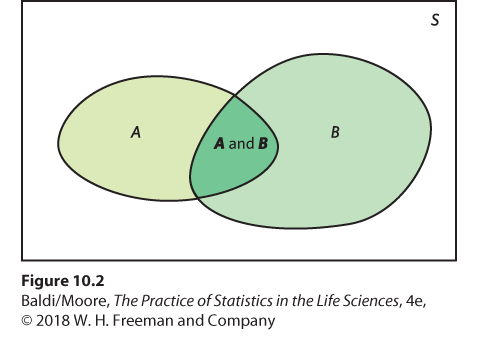
\includegraphics{figs/Venn1.png}

P(A) is the area of the circle labelled A, P(B) is the area of the
circle labelled B, and P(A and B) is the area of the overlap between
these two circles. P(A or B) is the total shaded area, including the
yellow-green, green, and dark green.

You can see the Addition Rule at work here. If you add the area of A
(which includes P(A and B)) to the area of B (which also includes P(A
and B)), you've added P(A and B) twice!

There are two formulas for P(A and B). The first one is found by
rearranging the formula for P(A or B):

\begin{align*}
\small P(A\; or\; B) &\small = P(A) + P(B) - P(A \;and\; B)\\
\small P(A\; and\; B) &\small = P(A) + P(B) - P(A \;or\; B)
\end{align*}

When in doubt, just remember P(A\_B) = P(A) + P(B) - P(A\_B), then put
``or'' in one blank and ``and'' in the other.

This formula won't always get you to the solution, though. There will be
many times where neither ``and'' nor ``or'' will be obvious, and we'll
need to do some more work to get them. We have special formulas for
``and'', so we'll usually try to figure out the ``and'' and then use it
to figure out the ``or''\footnote{This lecture has some of the weirdest
  sentences.}.

\hypertarget{given-conditional-probabilities}{%
\section{``given'': Conditional
Probabilities}\label{given-conditional-probabilities}}

A \emph{condition} is something that must happen before you can proceed.
A \textbf{conditional probability} is a probability that requires
something else to happen, and usually involves a more complicated setup.

Let's look at another scenario. Let's say I told you that the number on
the dice was larger than 3. What's the probability that the number on
the dice is a 4? Intuiutively, it's 1/3, since there are 3 possible
numbers. Our notation fails us here, P(4) denotes the probability that
the dice is a 4, which we already determined was 1/6. We can't use P(4)
for two things, so we need to add some notation.

In this case, the solution is to use a vertical bar, ``\textbar{}'',
which is pronounced ``given''. We write ``P(dice is 4 \textbar{} dice is
greater than 3) = 1/3'',\footnote{P(4 \textbar{} \textgreater3) just
  looks too confusing, so I added some words.} which is read as ``The
probability that the dice is 4, \textbf{given that} the dice is larger
than 3.''

A very important thing happened here: when we used a conditional
probability (``given that''), we \textbf{restricted the sample space}.
When we ``condition'' on an event, it means that we're only looking at
cases where that event happened. ``The probability that the dice is 4,
given that the dice is larger than 3'' is another way of saying that
we're only considering events where the dice roll is greater than 3; we
don't care about 1, 2, or 3.

We defined ``probability'' as the total number of events divided by the
total number of trials. For conditional probabilities, this means that
we're only looking at \emph{some of} the trials.

\begin{align*}
\small P(dice\; is\; 4\; |\; dice\; is >3) = \frac{\#\; ways\;dice\;can\;be\;4\;}{\#\;ways\;dice\;can\;be\;>3}=\frac{1}{3}
\end{align*}

\textbf{This formula is incorrect}: ``The number of ways that a dice can
be 4'' depends on the condition. For instance, the number of ways that a
dice can be 2 is 0 since we're told it's larger than 3. We are actually
looking at the number of ways that the dice can be both 4 \textbf{and}
greater than 3. Let's incorporate this information:

\begin{align*}
\small P(dice\; is\; 4\; |\; dice\; is >3) = \frac{\#\; ways\;dice\;can\;be\;4\;\;and\;>3}{\#\;ways\;dice\;can\;be\;>3}=\frac{1}{3}
\end{align*}

For any two events A and B, \textbf{conditional probabilities} are
defined as follows:\footnote{To remember this, I like to imagine the
  vertical bar falling on the the B and pushing it into the denominator.}

\begin{align*}
\small P(A | B) = \frac{P(A\;and\; B)}{P(B)}
\end{align*}

The equation above is a \emph{definition}. It's not the result of
something else, it's the way we define conditional probability.
Rearranging it, though, gives us an important result.

\hypertarget{and-part-2-the-multiplication-rule}{%
\section{``and'' Part 2: The Multiplication
Rule}\label{and-part-2-the-multiplication-rule}}

For any two events A and B, the \textbf{Multiplication Rule} states:

\begin{align*}
\small P(A\; and\; B) = P(A|B)P(B)
\end{align*}

Note that P(B\textbar A) = P(A and B)/P(A), so the multiplication rule
can be extended:

\begin{align*}
\small P(A\; and\; B) &\small = P(A|B)P(B)\\
\small P(A\; and\; B) &\small = P(B|A)P(A)
\end{align*}

In other words, you can write it either way as long as the event that
comes after the ``\textbar{}'' also appears on it's own.

Let's use this to answer the following question: What's the probability
that a dice is larger than 3 \textbf{and} even? By intuition, this
should be 2/6 since there are two cases where both are true, but let's
verify with math!

First, recall that P(\textgreater3) and P(even) are both 1/2.

P(\textgreater3 \textbar{} even) means that we're look at the number of
dice rolls that are larger than 3, but we're only considering even dice
rolls. We have 3 total dice rolls that are even, and 2 of those are
larger than 3, so this probability is 2/3. Using the multiplication
rule, P(\textgreater3 and even) = P(\textgreater3 \textbar{}
even)*P(even) = (2/3)*(1/2) = 2/6, which is what we got before!

The other way works out the same. Given that the roll is larger than 3,
there are 2 even rolls, which means that P(even \textbar{}
\textgreater3) = 2/3. P(\textgreater3 and even) = P(even \textbar{}
\textgreater3)*P(even) = (2/3)*(1/2) = 2/6, which is what we got before!

\hypertarget{special-cases-independent-or-disjoint}{%
\section{Special Cases: Independent or
Disjoint}\label{special-cases-independent-or-disjoint}}

\hypertarget{disjoint-a.k.a.-mutually-exclusive}{%
\subsection{Disjoint, a.k.a. Mutually
Exclusive}\label{disjoint-a.k.a.-mutually-exclusive}}

\textbf{Disjoint} events, also called \textbf{mutually exclusive}
events, are events that \emph{cannot} occur together. For example, the
event that you roll a 4 and it's also a 3. This simply does not work, so
the probability is 0.

More formally, A and B are \textbf{disjoint} if P(A and B) = 0.

\hypertarget{the-addition-rule-for-disjoint-events}{%
\subsection{The Addition Rule for Disjoint
Events}\label{the-addition-rule-for-disjoint-events}}

If A and B are disjoint, then P(A or B) = P(A) + P(B).\footnote{Not an
  important point: This is a rule, not a result. The General Addition
  Rule is a result of this rule, not the other way around.}

This is actually why we were able to say P(even) = P(2 or 4 or 6) = P(2)
+ P(4) + P(6) = 3/6: the events ``2'', ``4'', and ``6'' are disjoint.

\hypertarget{independent}{%
\subsection{Independent}\label{independent}}

Two events are \textbf{independent} if the knowledge of one event tells
you nothing about the other.\footnote{The opposite of
  \textbf{independence} is \textbf{dependence}.} For instance, if I flip
two different coins and tell you that the first one was Heads, you still
only have a 50/50 chance of guessing the second one.

Notice the phrasing in the previous sentence: ``If I tell you that the
first one is heads\ldots{}'' That is, I'm \emph{restricting the sample
space}. Independence is all about conditional probabilities!

Formally, A and B are independent if P(A \textbar{} B) = P(A).

This adds further insight into conditional probabilities: P(A\textbar B)
is how likely A is, given that you know B happened. Knowledge of B
changes your guess of the likelihood of A. If it doesn't change your
guess, then they are independent.\footnote{Just like in correlations,
  dependence does \emph{not} imply causation!}

The following app demonstrates this concept:

\begin{Shaded}
\begin{Highlighting}[]
\NormalTok{shiny}\SpecialCharTok{::}\FunctionTok{runGitHub}\NormalTok{(}\AttributeTok{repo =} \StringTok{"DBecker7/DB7\_TeachingApps"}\NormalTok{, }
    \AttributeTok{subdir =} \StringTok{"Apps/indep"}\NormalTok{)}
\end{Highlighting}
\end{Shaded}

Another lesson to take from the app above: Independence doesn't look
special. You can't just tell that things are independent by looking at
them.

\hypertarget{the-multiplication-rule-for-independent-events}{%
\subsection{The Multiplication Rule for Independent
Events}\label{the-multiplication-rule-for-independent-events}}

Any time I see a conditional probability, I immediately write down the
formula. For dependence, we are saying:

P(A\textbar B) = P(A and B)/P(B)

which is the same as

P(A and B) = P(A\textbar B)P(B)\footnote{This equation is \emph{always}
  true.}

If two events are \textbf{independent}, then P(A\textbar B)=P(A),
therefore:

P(A and B) \(\stackrel{indep}{=}\) P(A)*P(B)\footnote{The ``\(indep\)''
  over the equals sign is there to specify that this is only true if
  events are independent.}

Get this tattood backwards on your forehead so you see it every time you
look at yourself in the mirror: \textbf{P(A and B) is ONLY equal to
P(A)*P(B) when A and B are independent!!!} Some textbooks start with
this rule then move to the general rule, but far too many students start
using P(A and B) = P(A)P(B) as if it's always true. My entire thesis is
based on whether you can say two things are independent, so it's kind of
a sore spot for me. DO NOT MIX THIS UP.

For example, are the events ``even'' and ``\textgreater3'' independent?
If you know that the dice roll is \textgreater3, then there's a 2/3
chance that it's even. That is, P(even\textbar\textgreater3) = 2/3
\(\ne\) 1/2 = P(even), so it's not independent.

Alternatively, we can calcuate P(even and \textgreater3) = 2/3, but
P(even)*P(\textgreater3) = (1/2)*(1/2) = 1/4. Since 2/3 \(\ne\) 1/4,
these events are not independent.

\hypertarget{disjoint-means-dependent}{%
\subsection{\texorpdfstring{Disjoint means
\emph{Dependent}}{Disjoint means Dependent}}\label{disjoint-means-dependent}}

\textbf{Independence} can be defined as ``if you know that one event
happened, you have no knowledge of the other event.'' \textbf{Disjoint}
can be defined as ``if you know one event happened, you know for sure
that the other one \emph{did not} happen.'' If two events are disjoint,
they must be \textbf{dependent}. In fact, knowledge of one event means
that you for sure know about the other - the exact opposite of
independence!

\ldots{} except when one event is impossible. For instance, P(even and
7) = 0 since there are no dice rolls that are both even and 7, but this
is also equal to P(even)*P(7) = 0 since there are no dice rolls that are
7.

\hypertarget{word-problems}{%
\chapter{Word Problems}\label{word-problems}}

Question 10.6 from the textbook:\footnote{Baldi, B. and DS. Moore. 2018.
  \emph{The Practice of Statistics in the Life Sciences.} 4th Edition,
  W.H. Freeman and Company.}

The National Survey on Drug Use and Health reports that 18.1\% of all
adults in the United States had a mental illness in 2014. Among adults
with a substance use disorder, 39.1\% had a mental illness. By
comparison, only 16.2\% of adults without a substance use disorder had a
mental illness. The report also states that 3.3\% of American adults had
both a mental illness and a substance use disorder. Use the notation MI
and SUD for mental illness and substance abuse disorder, respectively.

\begin{enumerate}
\def\labelenumi{\alph{enumi}.}
\tightlist
\item
  Express the four percents cited here as probabilities for a randomly
  selected American adult. Use proper probability notation.
\item
  Obtain the probability P(SUD\textbar MI). Write a sentence reporting
  this probability in context.
\end{enumerate}

Solutions:

\begin{enumerate}
\def\labelenumi{\alph{enumi}.}
\tightlist
\item
  There are a couple of probabilities:

  \begin{itemize}
  \tightlist
  \item
    ``18.1\% of all adults in the United States had a mental illness'':
    P(MI) = 18.1
  \item
    ``Among adults with a substance use disorder, 39.1\% had a mental
    illness.'' The part that says ``among adults with SUD'' means that
    we're only looking at people with SUD; we're \emph{restricting the
    sample space}. This is a condition, so our answer must be P(\_
    \textbar{} SUD) = \_\_. The blanks can be filled in as
    P(MI\textbar SUD) = 0.391.
  \item
    ``16.2\% of adults without a substance use disorder had a mental
    illness.'' The part that says ``adults without a SUD'' is also
    \emph{restricting the sample space}, so our probability statement
    will be P(\_\_ \textbar{} no SUD) = \_\_. The blanks are filled in
    as P(MI \textbar{} no SUD) = 0.162.\footnote{This is a great place
      to mention: There's absolutely no reason why P(A\textbar B) +
      P(A\textbar{} not B) should add to 1.}
  \item
    ``3.3\% of American adults had both a MI and a SUD''. This clearly
    states \textbf{and}, so we are looking at P(MI and SUD) = 0.033
  \end{itemize}
\end{enumerate}

Part b. is going to take a few steps. Let's write down all the formulas
that might help. Firstly. there's no ``or'', so that probably won't do
it.

\begin{itemize}
\tightlist
\item
  \emph{Want}: P(SUD\textbar MI)

  \begin{itemize}
  \tightlist
  \item
    P(SUD\textbar MI) = P(SUD and MI)/P(MI), so we need P(SUD and MI)
    and P(MI).
  \end{itemize}
\item
  \emph{Have}:

  \begin{itemize}
  \tightlist
  \item
    P(MI) = 0.181
  \item
    P(MI \textbar{} SUD) = 0.391
  \item
    P(MI \textbar{} no SUD) = 0.162
  \item
    P(MI and SUD) = 0.033
  \end{itemize}
\end{itemize}

Both P(SUD and MI) and P(MI) are given in the question, so our answer is
simply:

\begin{quote}
P(SUD \textbar{} MI) = P(SUD and MI)/P(MI) = 0.033/0.181 = 0.1823
\end{quote}

Therefore 18.23\% of people with mental illness have substance abuse
disorder.

Compare this value to P(MI \textbar{} SUD) = 0.391. In general, there is
no easy relationship between P(A \textbar{} B) and P(B \textbar{} A). If
you know what P(A \textbar{} B) is, you can't really guess at what P(B
\textbar{} A) is; you need a lot more information!

\hypertarget{two-way-tables}{%
\chapter{Two-Way Tables}\label{two-way-tables}}

I rigorously collected the following data\footnote{Source: I made it up.}
on programming language usage for different disciplines using the most
appropriate sampling methods.

\begin{longtable}[]{@{}lllll@{}}
\toprule\noalign{}
& Stats & Math & Comp Sci & Total \\
\midrule\noalign{}
\endhead
\bottomrule\noalign{}
\endlastfoot
R & 90 & 30 & 40 & 160 \\
Python & 10 & 60 & 100 & 170 \\
MatLab & 15 & 60 & 15 & 90 \\
Julia & 10 & 10 & 1 & 21 \\
\textbf{Total} & 125 & 160 & 156 & 431 \\
\end{longtable}

From this table, we can calculate \textbf{marginal} and
\textbf{conditional} probabilities.

\textbf{Marginal} probabilities are calculated from the margins, which
means that we ignore one of the variables. For example, P(Math) =
160/431 and P(Julia) = 21/431. Both of these proportions are based on
the margins - they don't take the other variable into account.

\textbf{Conditional} probabilities are the same idea as we saw earlier.
Again, we are \emph{restricting our sample space} by conditioning on
another variable. For example, P(R \textbar{} Stats) = 90/125, whereas
P(Stats \textbar{} R) = 90/160. The conditioning event determines which
row/column we use. When we condition on Stats, we \emph{only} look at
the column labelled stats - we do not consider any of the other numbers.
This is why P(R \textbar{} Stats) has a numerator of 125, rather than
431.

You should be familiar with the following calculations:

\begin{enumerate}
\def\labelenumi{\arabic{enumi}.}
\tightlist
\item
  P(Stats) = 125/431
\item
  P(Stats \textbar{} Julia) = 10/21
\item
  P(Matlab \textbar{} Comp Sci) = ???\footnote{Answer is at the end.}
\item
  P(Stats \textbf{and} Julia) = 10/431
\item
  P(Matlab \textbf{and} Stats) = 15/431
\item
  P(Stats \textbf{or} Julia) = P(Stats) + P(Julia) - P(Stats
  \textbf{and} Julia) = 136/431
\item
  P(Matlab \textbf{or} Stats) = 200
\item
  P(Stats \textbf{or} R) = ???
\item
  P(Stats \textbf{or} Math) = ??
\end{enumerate}

Two-way tables can also be created in R using the \texttt{table()}
function:

\begin{Shaded}
\begin{Highlighting}[]
\FunctionTok{data}\NormalTok{(mtcars) }\CommentTok{\# It\textquotesingle{}s a very useful dataset}

\FunctionTok{cbind}\NormalTok{(mtcars}\SpecialCharTok{$}\NormalTok{am, mtcars}\SpecialCharTok{$}\NormalTok{cyl) }\CommentTok{\# cbind BINDs Columns together}
\end{Highlighting}
\end{Shaded}

\begin{verbatim}
      [,1] [,2]
 [1,]    1    6
 [2,]    1    6
 [3,]    1    4
 [4,]    0    6
 [5,]    0    8
 [6,]    0    6
 [7,]    0    8
 [8,]    0    4
 [9,]    0    4
[10,]    0    6
[11,]    0    6
[12,]    0    8
[13,]    0    8
[14,]    0    8
[15,]    0    8
[16,]    0    8
[17,]    0    8
[18,]    1    4
[19,]    1    4
[20,]    1    4
[21,]    0    4
[22,]    0    8
[23,]    0    8
[24,]    0    8
[25,]    0    8
[26,]    1    4
[27,]    1    4
[28,]    1    4
[29,]    1    8
[30,]    1    6
[31,]    1    8
[32,]    1    4
\end{verbatim}

\begin{Shaded}
\begin{Highlighting}[]
\FunctionTok{table}\NormalTok{(mtcars}\SpecialCharTok{$}\NormalTok{am, mtcars}\SpecialCharTok{$}\NormalTok{cyl)}
\end{Highlighting}
\end{Shaded}

\begin{verbatim}
   
     4  6  8
  0  3  4 12
  1  8  3  2
\end{verbatim}

The table above is telling us that there were 3 cars that were automatic
(0) \textbf{and} had 4 cylinders.

\begin{Shaded}
\begin{Highlighting}[]
\CommentTok{\# Note: TRUE == 1, so the sum of a logical vector is the number of TRUEs}
\CommentTok{\# The "\&" operator only returns true if BOTH conditions are true, i.e.}
\CommentTok{\# if mtcars$cyl == 4 AND mtcars$am == 0}
\FunctionTok{sum}\NormalTok{(mtcars}\SpecialCharTok{$}\NormalTok{cyl }\SpecialCharTok{==} \DecValTok{4} \SpecialCharTok{\&}\NormalTok{ mtcars}\SpecialCharTok{$}\NormalTok{am }\SpecialCharTok{==} \DecValTok{0}\NormalTok{)}
\end{Highlighting}
\end{Shaded}

\begin{verbatim}
[1] 3
\end{verbatim}

\hypertarget{self-study-questions}{%
\chapter{Self-Study Questions}\label{self-study-questions}}

\begin{enumerate}
\def\labelenumi{\arabic{enumi}.}
\tightlist
\item
  Explain why P(A) + P(not A) must be 1.
\item
  If P(A) = 0.2, P(B) = 0.35,

  \begin{enumerate}
  \def\labelenumii{\alph{enumii}.}
  \tightlist
  \item
    and P(A or B) = 0.75, find P(A and B).
  \item
    and P(A and B) = 0.15, find P(A or B).
  \item
    explain why P(A and B) can only be as large as 0.2.
  \item
    explain why P(A or B) must be at least 0.35.
  \end{enumerate}
\item
  For a 6-sided dice, show that the events ``even'' and ``odd'' are
  \emph{not} independent.
\item
  For a 6-sided dice, show that the events ``even'' and
  ``\textgreater4'' \emph{are} independent.
\item
  Consider flipping one coin and rolling one dice.

  \begin{enumerate}
  \def\labelenumii{\alph{enumii}.}
  \tightlist
  \item
    List out all possible events (e.g., H1 for heads and 1, T4 for tails
    and a 4 on the dice).
  \item
    Based on your sample space, argue that P(T1) = 1/12.
  \item
    Are the events ``coin is tails'' and ``dice is 1'' independent? Give
    an intuitive and a mathematical reason.
  \end{enumerate}
\item
  Consider a loaded dice, where the probability of 1, 2, 3, 4, and 5 are
  all 1/8.

  \begin{enumerate}
  \def\labelenumii{\alph{enumii}.}
  \tightlist
  \item
    Explain why P(6) must be 3/8.
  \item
    What is P(even)?
  \item
    Are the events ``even'' and ``\textless3'' independent?
  \end{enumerate}
\end{enumerate}

Solutions to Two-Way Table exercises: \textbf{3.} 15/156; \textbf{8.}
195/431; \textbf{9.} 185/431

\hypertarget{the-normal-distributions-part-1}{%
\chapter{The Normal Distributions (Part
1)}\label{the-normal-distributions-part-1}}

\hypertarget{introduction-2}{%
\chapter{Introduction}\label{introduction-2}}

In this lecture we are looking at continuous distributions. Continuous
distributions have an odd quirk. If a variable has a continuous
distribution, then \(P(X = x) = 0\). That is, the probability of any
specific value is infinitely small.

Think of it this way: suppose that human heights go from 54 cm to 272
cm. For now, suppose all of these heights are equally likely. If we
record heights to the nearest centimeter, there are 219 possible
heights, so the probability that you are one of those heights is 1/219.
If we round to the nearest mm, there are 21,900 different heights. As we
get a more and more accurate measuring instrument, the probability of
any given height goes to 0. It's not that these heights are impossible,
it's that you're probably not going to ever guess my exact height when
we measure it with infinite accuracy.

So what do we do? How could we possibly calculate probabilities? Well,
we measure ranges! You can't guess my height exactly, but we can talk
about the probability that my height is between 170 and 180 cm, or even
the probability that my height would be 170, assuming we round to the
nearest centimeter.

\hypertarget{some-facts-about-distributions}{%
\section{Some Facts about
Distributions}\label{some-facts-about-distributions}}

Before we begin, the following properties are true of \emph{any}
distribution, regardless of whether they are discrete or continuous.

\begin{enumerate}
\def\labelenumi{\arabic{enumi}.}
\tightlist
\item
  All probabilities must be between 0 and 1.
\item
  All probabilities together must make 1.

  \begin{itemize}
  \tightlist
  \item
    For discrete, adding them all should get you to 1.
  \item
    For continuous, the area under the density curve must be
    1.\footnote{This is done with integrals, but we won't actually do
      this in this course.}
  \end{itemize}
\item
  If two events are disjoint, you must be able to add their
  probabilities.

  \begin{itemize}
  \tightlist
  \item
    It's weird, but we have to define this as a rule first before we can
    calculate probabilities.
  \end{itemize}
\end{enumerate}

The first point should be obvious, and you won't ever need to check
whether the third point is true.

The second point is the important one: The total probability for all
events must be 1. For continuous distributions like the normal
distribution, that means that the area under the curve is 1.\footnote{For
  continuous distributions, ``probability'' and ``area under the curve''
  are synonyms.}

\hypertarget{the-normal-distribution}{%
\chapter{The Normal Distribution}\label{the-normal-distribution}}

The normal distribution is a way to define the probability of something
using a function, but the function is complicated.\footnote{\((2\pi\sigma^2)^{-1/2}\exp\left(\frac{(x-\mu)^2}{-2\sigma^2}\right)\)}
Instead, we'll jump right into how to use it and let software deal with
the function.

In the introduction, I used the example of people's heights. I made the
assumption that all heights were equally likely, but this is just a
bonkers thing to say. Instead, some heights are more likely than other
heights. Of course, this doesn't mean that, say, 170 cm is very
unlikely, but 175 is likely, then 176 is unlikely, then 177 is
\emph{very} unlikely, then 178 is suddenly really likely again; most
people have heights close to the average and heights further from the
average are less likely. This is exactly what the normal distribution is
for! Here's what the normal distribution looks like:

\begin{Shaded}
\begin{Highlighting}[]
\NormalTok{mu }\OtherTok{\textless{}{-}} \FloatTok{162.3}
\NormalTok{sig }\OtherTok{\textless{}{-}} \FloatTok{7.11}
\NormalTok{xseq }\OtherTok{\textless{}{-}} \FunctionTok{seq}\NormalTok{(mu}\DecValTok{{-}3}\SpecialCharTok{*}\NormalTok{sig, mu }\SpecialCharTok{+} \DecValTok{3}\SpecialCharTok{*}\NormalTok{sig, }\AttributeTok{length.out =} \DecValTok{300}\NormalTok{)}
\NormalTok{yseq }\OtherTok{\textless{}{-}} \FunctionTok{dnorm}\NormalTok{(}\AttributeTok{x =}\NormalTok{ xseq, }\AttributeTok{mean =}\NormalTok{ mu, }\AttributeTok{sd =}\NormalTok{ sig) }

\FunctionTok{plot}\NormalTok{(xseq, yseq, }\AttributeTok{type =} \StringTok{"l"}\NormalTok{,}
  \AttributeTok{main =} \StringTok{"Heights of Canadian Women"}\NormalTok{,}
  \AttributeTok{xlab =} \StringTok{"Height (cm)"}\NormalTok{, }\AttributeTok{ylab =} \StringTok{"Prob. Density"}\NormalTok{)}
\end{Highlighting}
\end{Shaded}

\begin{figure}[H]

{\centering \includegraphics{L07-Normal-1_files/figure-pdf/unnamed-chunk-1-1.pdf}

}

\end{figure}

The plot above has the highest point occurs at exactly 162.3, which is
the best number I could find for the actual average height of Canadian
women. This is denoted \(\mu\). The width of the curve is a little
trickier - how did I choose to make it go from 145 to 180? I could
easily have stretched it out or squeezed it inwards in both directions.
The width is defined by the standard deviation, which is denoted
\(\sigma\). Because of the way the normal distribution is defined,
there's nothing else we can change about it - knowing \(\mu\) and
\(\sigma\) are enough to draw the entire curve.

\begin{Shaded}
\begin{Highlighting}[]
\CommentTok{\# Requires the "shiny" library}
\NormalTok{shiny}\SpecialCharTok{::}\FunctionTok{runGitHub}\NormalTok{(}\AttributeTok{repo =} \StringTok{"DBecker7/DB7\_TeachingApps"}\NormalTok{, }
    \AttributeTok{subdir =} \StringTok{"Tools/normShape"}\NormalTok{)}
\end{Highlighting}
\end{Shaded}

If we have a variable \(X\) that follows a normal distribution, we use
the notation \(X \sim N(\mu, \sigma)\).

\begin{tcolorbox}[enhanced jigsaw, opacitybacktitle=0.6, left=2mm, colbacktitle=quarto-callout-warning-color!10!white, colframe=quarto-callout-warning-color-frame, breakable, toptitle=1mm, title=\textcolor{quarto-callout-warning-color}{\faExclamationTriangle}\hspace{0.5em}{Warning}, opacityback=0, bottomrule=.15mm, toprule=.15mm, arc=.35mm, leftrule=.75mm, titlerule=0mm, bottomtitle=1mm, colback=white, rightrule=.15mm, coltitle=black]

Some textbooks use the notation \(X \sim N(\mu, \sigma^2)\), i.e.~they
use \(\sigma^2\) rather than \(\sigma\). It's like driving on the left
or the right side of the road - both are fine, but we have to choose one
and stick with it.

\end{tcolorbox}

The idea that ``most things are close to the center, and fewer things
further away'' can be very powerful. This applies to:

\begin{itemize}
\tightlist
\item
  Human heights
\item
  Income for a given job position
\item
  Change in stock price from day to day

  \begin{itemize}
  \tightlist
  \item
    On average the change is 0, but it does change. Small changes are
    much more likely than large ones, but large ones do happen.
  \item
    Obviously, extreme events happen sometimes, and major changes can
    happen.
  \end{itemize}
\item
  IQ scores
\item
  Birth weight
\item
  How much the prediction of a model differs from the truth
\end{itemize}

\hypertarget{calculating-normal-probabilities---part-1}{%
\chapter{Calculating Normal Probabilities - Part
1}\label{calculating-normal-probabilities---part-1}}

The height and width of the normal distribution are determined by the
\textbf{mean} (\(\mu\)) and \textbf{standard deviation} (\(\sigma\)),
and \emph{only} the mean and standard deviation. The mean just moves the
curve left and right, the standard deviation squeezes or stretches it.

To highlight this, we introduce something called the \textbf{Empirical
Rule}, a.k.a. the 68-95-99.5 Rule. No matter what the mean of the
distribution is, 68\% of the probability is within 1 standard deviation
of the mean. To say this another way, let's extend our notation
slightly. If \(X\sim N(\mu,\sigma)\), we can say that:

\begin{align*}
P(\mu - \sigma \le X \le \mu + \sigma) \approx 0.68
\end{align*}

To phrase this in another way, if we were to draw random numbers from
the normal distribution, 68\% of them would be between 1sd below the
mean and 1sd above the mean.

\begin{Shaded}
\begin{Highlighting}[]
\FunctionTok{set.seed}\NormalTok{(}\SpecialCharTok{{-}}\DecValTok{4}\NormalTok{) }\CommentTok{\# Ensure the same random numbers every time}

\CommentTok{\# generate 10000 random N(0,1) values}
\NormalTok{x }\OtherTok{\textless{}{-}} \FunctionTok{rnorm}\NormalTok{(}\AttributeTok{n =} \DecValTok{10000}\NormalTok{, }\AttributeTok{mean =} \DecValTok{0}\NormalTok{, }\AttributeTok{sd =} \DecValTok{1}\NormalTok{) }

\CommentTok{\# You won\textquotesingle{}t need to know how to write this code:}
\FunctionTok{sum}\NormalTok{(x }\SpecialCharTok{\textgreater{}} \SpecialCharTok{{-}}\DecValTok{1} \SpecialCharTok{\&}\NormalTok{ x }\SpecialCharTok{\textless{}} \DecValTok{1}\NormalTok{) }\CommentTok{\# x is larger than {-}1 AND less than 1}
\end{Highlighting}
\end{Shaded}

\begin{verbatim}
[1] 6766
\end{verbatim}

So out of 10,000 random numbers from a N(0,1) distribution, 6,766
(67.66\%) of them were above -1 but below 1. If we change the mean and
sd, we still get the same results:

\begin{Shaded}
\begin{Highlighting}[]
\CommentTok{\# Mean is 4, sd is 30, so mean {-} 1sd = 4 {-} 30}
\CommentTok{\# Change the mean and sd for yourself to see what happens!}
\NormalTok{mu }\OtherTok{\textless{}{-}} \DecValTok{4}
\NormalTok{sigma }\OtherTok{\textless{}{-}} \DecValTok{30}
\NormalTok{x2 }\OtherTok{\textless{}{-}} \FunctionTok{rnorm}\NormalTok{(}\AttributeTok{n =} \DecValTok{10000}\NormalTok{, }\AttributeTok{mean =}\NormalTok{ mu, }\AttributeTok{sd =}\NormalTok{ sigma)}
\FunctionTok{sum}\NormalTok{(x2 }\SpecialCharTok{\textgreater{}}\NormalTok{ (mu }\SpecialCharTok{{-}}\NormalTok{ sigma) }\SpecialCharTok{\&}\NormalTok{ x2 }\SpecialCharTok{\textless{}}\NormalTok{ (mu }\SpecialCharTok{+}\NormalTok{ sigma)) }\CommentTok{\# Not exactly 68\%, but approximate!}
\end{Highlighting}
\end{Shaded}

\begin{verbatim}
[1] 6845
\end{verbatim}

As you can guess from the name ``68-95-99.7 Rule'', 68\% being within
one sd is only part of the story. The 95 refers to 95\% being within 2sd
of the mean, and the 99.7 refers to 99.7\% being within 3sd of the mean.

\begin{Shaded}
\begin{Highlighting}[]
\FunctionTok{sum}\NormalTok{(x }\SpecialCharTok{\textgreater{}} \SpecialCharTok{{-}}\DecValTok{2} \SpecialCharTok{\&}\NormalTok{ x }\SpecialCharTok{\textless{}} \DecValTok{2}\NormalTok{) }\CommentTok{\# within 2sd of the mean}
\end{Highlighting}
\end{Shaded}

\begin{verbatim}
[1] 9523
\end{verbatim}

\begin{Shaded}
\begin{Highlighting}[]
\FunctionTok{sum}\NormalTok{(x }\SpecialCharTok{\textgreater{}} \SpecialCharTok{{-}}\DecValTok{3} \SpecialCharTok{\&}\NormalTok{ x }\SpecialCharTok{\textless{}} \DecValTok{3}\NormalTok{) }\CommentTok{\# within 3}
\end{Highlighting}
\end{Shaded}

\begin{verbatim}
[1] 9970
\end{verbatim}

\begin{Shaded}
\begin{Highlighting}[]
\CommentTok{\# Try this with x2 as well!}
\end{Highlighting}
\end{Shaded}

Some variant of the following image appears in countless textbooks:

\includegraphics{figs/emprirical.png}

As a small side note, the image above uses the word ``data''. By this,
it means that if this is the \textbf{population}, then 68\% of all the
data that it were possible to collect would be within one standard
deviation of the mean. As we saw in the simulated data above, this
number is almost never going to be perfect.

\hypertarget{trickier-calculations}{%
\section{Trickier calculations}\label{trickier-calculations}}

If 68\% of the data is between \(\mu - \sigma\) and \(\mu + \sigma\),
then there's still 32\% of the distribution outside this range. The
normal distribution is \textbf{symmetric}, so this 32\% gets split
exactly in half and 16\% of the distribution is below \(\mu - \sigma\),
and 16\% is above \(\mu + \sigma\).

Based on this calculation, we can say that 84\% of any normal
distribution is below \(\mu + \sigma\), and 84\% is above
\(\mu - \sigma\). Before we move on, draw out some normal distributions
to convince yourself that 97.5\% of any normal distribution is less than
\(\mu + 2\sigma\).\footnote{I generally keep a running tally of the
  number of normal distributions I draw on the board. Last time I did
  this, I was almost at 100. The moral: you should be drawing a lot of
  normal distributions!!!}

You should try the following calculations yourself, all of which can be
done with basic arithmetic and the 68-95-99.7 Rule:

\begin{enumerate}
\def\labelenumi{\arabic{enumi}.}
\tightlist
\item
  Below \(\mu+2\sigma\) and above \(\mu-\sigma\).
\item
  Below \(\mu+2\sigma\) and above \(\mu+\sigma\).
\item
  Above \(\mu + 2\sigma\) and below \(\mu + 3\sigma\)
\item
  Above \(\mu - 3\sigma\) and below 0.
\end{enumerate}

\hypertarget{the-standard-normal-distribution}{%
\chapter{The Standard Normal
Distribution}\label{the-standard-normal-distribution}}

We use a special letter (Z, pronounced ``zed'' because we're Canadian)
to denote a standard normal distribution. In particular,
\(Z\sim N(0, 1)\) is a normal distribution with mean 0 and standard
deviation 1. Many many many many textbooks have a table in the back of
them that gives probabilities for the standard normal distribution, and
they call them \(Z\) tables.

All normal distributions have the exact same shape. In order to change
the mean and sd, we can simply re-write the numbers on the axes. If we
want to shift the whole curve to the left by 2 units, we can re-label
the numbers on the x axis. If we change the sd, the plot might get
``taller'' or ``shorter'', but if we zoom in on the plot we can make it
look exactly the same!\footnote{This is also the reason why the
  empirical rule works! If you change the labels on the plot,
  \(\mu+\sigma\) stays in the same place so you can calculate the same
  probability.}

\hypertarget{standardizing-a-normal-distribution}{%
\section{Standardizing a Normal
Distribution}\label{standardizing-a-normal-distribution}}

Because they all look the same, we might as well work with just one of
them! Suppose \(X\sim N(\mu,\sigma)\). If we shift the whole curve to
the left, then the mean shifts as well and the mean is 0. In other
words, \(X-\mu \sim N(0,\sigma)\). Now that the mean is at 0,
\(\mu + 1\sigma\) is simply \(\sigma\), \(\mu-3\sigma\) is \(-3\sigma\),
and so on. If we divide all of the numbers by \(\sigma\), then
\(\sigma\) is simply 1, \(-3\sigma\) is simply -3, and so on. To
formalize this, if \(x\sim N(\mu,\sigma)\), then

\begin{align*}
\frac{X-\mu}{\sigma} = Z \sim N(0, 1)
\end{align*}

This is called \textbf{standardizing} a normal distribution. The
resultant value is called the \textbf{z-score}.

For example, suppose a woman is 155.19 cm tall. If the true mean height
of Canadian women is 162.3 and the standard deviation is 7.11, then this
particular woman is exactly one standard deviation \emph{below} the
mean. This is the \textbf{z-score}, a.k.a. the standardized value; this
woman's z-score is -1.

Now consider a woman who is 161.22 cm tall. Her z-score would be
-0.152,\footnote{The negative is important!} meaning that she is 0.152
standard deviations below the mean.

Let's return to the 155.19 cm tall woman. If you take a woman at random
from the population, what is the probability that the randomly chosen
woman be be shorter than 155.19 cm? Based on the 68-95-99.7 rule, 68\%
of women are within one standard deviation of the mean, which is a range
from 155.19 to 169.41. Since 68\% of the women are betwen these two
numbers, 16\% of them are shorter than 155.19 (it is also true that 16\%
are taller than 169.41, but this was not required for the question).

Now, what's the probability that a randomly chosen woman is, say,
shorter than 160 cm? This doesn't fit nicely in the empirical rule, so
we need another way to calculate probabilities. However, it's worth
stopping and trying to make a guess! The empirical rule tells us that
16\% of women are below 155.19 cm, and we also know that 50\% of women
are shorter than the average of 162.3 cm (since the normal distribution
is symmetric), so we expect that the answer is somewhere between 16\%
and 50\%, probably closer to 50\% since 160 cm is closer to 162.3 cm
than it is to 155.19 cm.

\hypertarget{calculating-normal-probabilities---part-2}{%
\chapter{Calculating Normal Probabilities - Part
2}\label{calculating-normal-probabilities---part-2}}

In general, we use the \textbf{cumulative distribution function} (CDF,
or cdf) to calculate probabilities. As with the cumulative probability
tables we saw in the probability lectures, the cumulative probability
calculates the area to the \emph{left} of a particular point.\footnote{Recall
  that \(P(X=x) = 0\) in continuous distributions, so we look at ranges.}
Questions about the normal distribution generally come in three
flavours:

\begin{enumerate}
\def\labelenumi{\arabic{enumi}.}
\tightlist
\item
  Find \(P(X \le a)\)
\item
  Find \(P(X \ge b)\)
\item
  Find \(P(c \le X\le d)\)
\end{enumerate}

The \textbf{cdf} is defined as \(P(X\le x)\), which allows us to answer
questions like 1. For the standard normal distribution, a table of Z
probabilities can be found at the back of the textbook. I've added a
file that demonstrates how to use the Z-table in the Lecture Materials.
This is something that is crucial to know for closed-book tests since
you will need to caclulate probabilities somehow, but we can't let you
have a computer to run R! Before moving on, read ``\textbf{Intro to
Ztable.pdf}''.

In that file, there are some practice problems. Below, you'll find a
selection of solutions using R. For your own practice, try and calculate
them with the Z-table (with some good drawings) and verify your answer
with R.

\begin{Shaded}
\begin{Highlighting}[]
\CommentTok{\# 1. Find the probability of a z{-}value less than 1.11.}
\FunctionTok{pnorm}\NormalTok{(}\FloatTok{1.11}\NormalTok{)}
\end{Highlighting}
\end{Shaded}

\begin{verbatim}
[1] 0.8665005
\end{verbatim}

\begin{Shaded}
\begin{Highlighting}[]
\CommentTok{\# 2. Find the probability of a z{-}value greater than 1.11}
\DecValTok{1} \SpecialCharTok{{-}} \FunctionTok{pnorm}\NormalTok{(}\FloatTok{1.11}\NormalTok{)}
\end{Highlighting}
\end{Shaded}

\begin{verbatim}
[1] 0.1334995
\end{verbatim}

\begin{Shaded}
\begin{Highlighting}[]
\CommentTok{\# 3. Find the probability of a z{-}value greater than {-}2.01 but less than 1.}
\FunctionTok{pnorm}\NormalTok{(}\DecValTok{1}\NormalTok{) }\SpecialCharTok{{-}} \FunctionTok{pnorm}\NormalTok{(}\SpecialCharTok{{-}}\FloatTok{2.01}\NormalTok{)}
\end{Highlighting}
\end{Shaded}

\begin{verbatim}
[1] 0.8191292
\end{verbatim}

\begin{Shaded}
\begin{Highlighting}[]
\CommentTok{\# 4. Verify the empirical rule: 68{-}95{-}99.7}
\FunctionTok{pnorm}\NormalTok{(}\DecValTok{1}\NormalTok{) }\SpecialCharTok{{-}} \FunctionTok{pnorm}\NormalTok{(}\SpecialCharTok{{-}}\DecValTok{1}\NormalTok{)}
\end{Highlighting}
\end{Shaded}

\begin{verbatim}
[1] 0.6826895
\end{verbatim}

\begin{Shaded}
\begin{Highlighting}[]
\FunctionTok{pnorm}\NormalTok{(}\DecValTok{2}\NormalTok{) }\SpecialCharTok{{-}} \FunctionTok{pnorm}\NormalTok{(}\SpecialCharTok{{-}}\DecValTok{2}\NormalTok{)}
\end{Highlighting}
\end{Shaded}

\begin{verbatim}
[1] 0.9544997
\end{verbatim}

\begin{Shaded}
\begin{Highlighting}[]
\FunctionTok{pnorm}\NormalTok{(}\DecValTok{3}\NormalTok{) }\SpecialCharTok{{-}} \FunctionTok{pnorm}\NormalTok{(}\SpecialCharTok{{-}}\DecValTok{3}\NormalTok{)}
\end{Highlighting}
\end{Shaded}

\begin{verbatim}
[1] 0.9973002
\end{verbatim}

For questions like \(P(X\ge x)\), we can simply use the fact that
\(P(X \ge x) = 1 - P(X<x)\). Since this is a continuous distribution and
\(P(X = x)=0\), we also know that \(P(X\le x) = P(X<x)\) and we can just
use the cdf. The last one is a little bit trickier.

To calculate the probability that a randomly chosen value will be within
a given range, there are a few steps. Let's use the same example as the
textbook: If \(X\sim N(-2, 1)\) find \(P(-2.5\le X\le -1)\). If we want
to use the cdf, we need to re-write this in terms of \(P(X\le x)\).

Here's how we do it. If we only find \(P(X\le-1)\), then we have taken
too much of the distribution. Everything to the left of -2.5 was
something that should not have been included. So why don't we just
remove it? By this logic, we find
\(P(-2.5\le X \le -1) = P(X\le -1) - P(X \le -2.5)\). This is shown
graphically below:

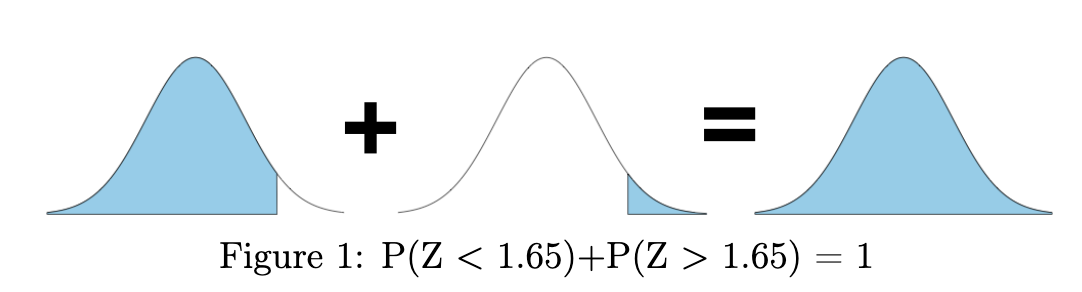
\includegraphics{figs/addgraphs.png}

Returning to the heights example, the probability of a randomly chosen
woman being less than 160 cm can be calculated as: \[
\frac{x - \mu}{\sigma} = \frac{160 - 162.3}{7.11} = -0.323488045
\] We can now look up -0.323 on the normal table. Try that out, and
verify that you get the same value here:

\begin{Shaded}
\begin{Highlighting}[]
\FunctionTok{pnorm}\NormalTok{(}\SpecialCharTok{{-}}\FloatTok{0.323488045}\NormalTok{)}
\end{Highlighting}
\end{Shaded}

\begin{verbatim}
[1] 0.3731628
\end{verbatim}

Note that R will do the standardization for you if you ask it politely.

\begin{Shaded}
\begin{Highlighting}[]
\FunctionTok{pnorm}\NormalTok{(}\AttributeTok{q =} \DecValTok{160}\NormalTok{, }\AttributeTok{mean =} \FloatTok{162.3}\NormalTok{, }\AttributeTok{sd =} \FloatTok{7.11}\NormalTok{)}
\end{Highlighting}
\end{Shaded}

\begin{verbatim}
[1] 0.3731628
\end{verbatim}

I have created a shiny app that lets you explore these
calculations\footnote{If you're curious, yes I've made a lot of Shiny
  apps. You can find them all here:
  \url{https://github.com/DBecker7/DB7_TeachingApps}}. Feel free to use
this to answer the questions in this lecture, and then double check the
answers with the z-table.

\begin{Shaded}
\begin{Highlighting}[]
\CommentTok{\# install.packages("shiny") \# Run this if you get an error about "package not found"}
\NormalTok{shiny}\SpecialCharTok{::}\FunctionTok{runGitHub}\NormalTok{(}\AttributeTok{repo =} \StringTok{"DBecker7/DB7\_TeachingApps"}\NormalTok{, }
    \AttributeTok{subdir =} \StringTok{"Tools/pnorm"}\NormalTok{)}
\end{Highlighting}
\end{Shaded}

\hypertarget{examples-1}{%
\section{Examples}\label{examples-1}}

\hypertarget{ex1-px-x}{%
\subsection{Ex1: P(X \textless{} x)}\label{ex1-px-x}}

\begin{enumerate}
\def\labelenumi{\arabic{enumi}.}
\tightlist
\item
  If X has a mean of 4 and a sd of 2, what's the probability of a value
  less than 0?

  \begin{itemize}
  \tightlist
  \item
    \textbf{Solution 1}: Standardize and Z-table. I'll split this up
    into steps:

    \begin{enumerate}
    \def\labelenumii{\arabic{enumii}.}
    \tightlist
    \item
      Standardize: \((x-\mu)/\sigma = (0 - 4)/2 = -2\).
    \item
      Find -2 on the Z table: -2=-2.00, so this will be in the row
      labelled -2.0 and the column labelled 0.00,\footnote{The rows are
        the digits before and after the decimal, the column is the
        second digit after the decimal.} which is 0.0228.
    \item
      Conclude: 2.28\% of the N(4,2) distribution is below 0.
    \end{enumerate}
  \item
    \textbf{Solution 2}: Empircal rule.

    \begin{itemize}
    \tightlist
    \item
      Before calculating a normal probability, try and estimate how many
      standard deviations away from the mean the value is. In this case,
      0 is 2 standard deviations from 4. The 68-95-99.7 rule states that
      95\% of the distribution is outside the range from
      \(\mu - 2\sigma\) to \(\mu + 2\sigma\), so 5\% is outside of this
      range. This means that 2.5\% is on either side, which means that
      2.5\% is below 0.
    \end{itemize}
  \end{itemize}
\end{enumerate}

A short version of Solution 2: By the 68-95-99.7 Rule, 95\% is between 0
and 8. Therefore, 2.5\% must be less than 0.

As you can see, the 68-95-99.7 rule is \emph{approximate}. However, I
highly recommend doing many practice problems with it. On a multiple
choice question, if you can figure out the answer with the Empirical
Rule than you might be able to guess the correct answer much quicker.
You won't get the exact answer, but if there's only one answer that's
close to your guess, then that's probably it.\footnote{You need to trust
  your ability to use the Empirical Rule, though.}

\textbf{Solution 3}: R.

\begin{Shaded}
\begin{Highlighting}[]
\CommentTok{\# Standardize:}
\FunctionTok{pnorm}\NormalTok{((}\DecValTok{0} \SpecialCharTok{{-}} \DecValTok{4}\NormalTok{)}\SpecialCharTok{/}\DecValTok{2}\NormalTok{)}
\end{Highlighting}
\end{Shaded}

\begin{verbatim}
[1] 0.02275013
\end{verbatim}

\begin{Shaded}
\begin{Highlighting}[]
\CommentTok{\# Same answer, without standardizing:}
\FunctionTok{pnorm}\NormalTok{(}\AttributeTok{q =} \DecValTok{0}\NormalTok{, }\AttributeTok{mean =} \DecValTok{4}\NormalTok{, }\AttributeTok{sd =} \DecValTok{2}\NormalTok{)}
\end{Highlighting}
\end{Shaded}

\begin{verbatim}
[1] 0.02275013
\end{verbatim}

\begin{enumerate}
\def\labelenumi{\arabic{enumi}.}
\setcounter{enumi}{1}
\tightlist
\item
  If \(X\sim N(1234, 56)\), what's the probability of a number smaller
  than 1432.
\end{enumerate}

\emph{Before we begin:} What do we expect the number to be? The mean is
1234, which is smaller than 1432. Is it a little smaller, or is it a lot
smaller? Compared to the standard deviation, it's a lot smaller. By the
empirical rule, the vast majority of the distribution is below
\(\mu + 3\sigma\), which is approximately 1400.\footnote{Quick maths -
  we're just trying to get an okay guess, not the exact answer right
  now.} We should expect an answer close to 1, since the area under the
normal distribution is 1.

\textbf{Solution 1}: \((x-\mu)/\sigma = (1432-1234)/56 = 3.54\), which
is not on the Z table. When this happens (and we don't have access to
technology), we simply say the answer is 1.\footnote{If the z-score were
  -3.54, we'd say the probability is 0.}

\textbf{Solution 2}: The value we're interested in isn't 1, 2, or 3
standard deviations from the mean, so the Empirical Rule doesn't apply.
However, we can guess that our probability will be close to 1 since it's
larger than 3 standard deviations away.

\textbf{Solution 3}: R.

\begin{Shaded}
\begin{Highlighting}[]
\FunctionTok{pnorm}\NormalTok{(}\DecValTok{1432}\NormalTok{, }\AttributeTok{mean =} \DecValTok{1234}\NormalTok{, }\AttributeTok{sd =} \DecValTok{56}\NormalTok{)}
\end{Highlighting}
\end{Shaded}

\begin{verbatim}
[1] 0.9997967
\end{verbatim}

Ideally, you would only ever use intuition from the Empirical rule, or
use R. The Z-table is super convenient for written, in-person exams.
It's also nice for situations where you don't have a computer with R
available.

\hypertarget{px-x}{%
\subsection{P(X \textgreater{} x)}\label{px-x}}

\begin{enumerate}
\def\labelenumi{\arabic{enumi}.}
\setcounter{enumi}{2}
\tightlist
\item
  If X has a mean of 4 and a sd of 2, what's the probability of a value
  greater than 0?
\end{enumerate}

\emph{Before we start}: Use the empirical rule! 0 is 2sd below the mean,
so the answer should be close to 97.5\%

\textbf{With the Z table}: \((x-\mu)/\sigma = -2\), and we've already
found this on the table as 0.0228. Since we're looking at the
\textbf{right tail}, our answer is 1 - 0.0228 = 0.9772.

\textbf{With R}:

\begin{Shaded}
\begin{Highlighting}[]
\DecValTok{1} \SpecialCharTok{{-}} \FunctionTok{pnorm}\NormalTok{(}\DecValTok{0}\NormalTok{, }\AttributeTok{mean =} \DecValTok{4}\NormalTok{, }\AttributeTok{sd =} \DecValTok{2}\NormalTok{)}
\end{Highlighting}
\end{Shaded}

\begin{verbatim}
[1] 0.9772499
\end{verbatim}

\begin{enumerate}
\def\labelenumi{\arabic{enumi}.}
\setcounter{enumi}{3}
\tightlist
\item
  Suppose \(X\sim N(23, 23)\). What's the probability of a value larger
  than 23?
\end{enumerate}

\emph{Before we start}: The normal distribution is perfectly symmetric,
which we have learned means that the mean is equal to the median. The
median marks the point where 50\% of the distribution is smaller. So
before doing any work, we know that the answer must be 50\%

\begin{Shaded}
\begin{Highlighting}[]
\FunctionTok{pnorm}\NormalTok{(}\DecValTok{23}\NormalTok{, }\DecValTok{23}\NormalTok{, }\DecValTok{23}\NormalTok{)}
\end{Highlighting}
\end{Shaded}

\begin{verbatim}
[1] 0.5
\end{verbatim}

\hypertarget{pa-x-b}{%
\subsection{P(a \textless{} X \textless{} b)}\label{pa-x-b}}

\begin{enumerate}
\def\labelenumi{\arabic{enumi}.}
\setcounter{enumi}{4}
\tightlist
\item
  If \(X\sim N(0, 1)\), what's the probability of a value between -1.52
  and -0.5?
\end{enumerate}

\textbf{Solution 1}: We have a standard normal value, so we can look
these values up directly. P(Z \textless{} -1.52) = 0.0643\footnote{Row
  labelled -1.5, column labelled 0.02.} and P(Z \textless{} -0.5) =
0.3085.\footnote{Verify this!} We want the area between these two
values. P(Z \textless{} -0.5) contains everything from negative infinity
to -0.5, but we only want values from -1.52 to -0.5. To fix this, we
remove everything from negative infinity to -1.52. Our answer is 0.3085
- 0.0643 = 0.2442.

\textbf{Solution 2}: R.

\begin{Shaded}
\begin{Highlighting}[]
\FunctionTok{pnorm}\NormalTok{(}\SpecialCharTok{{-}}\FloatTok{0.5}\NormalTok{) }\SpecialCharTok{{-}} \FunctionTok{pnorm}\NormalTok{(}\SpecialCharTok{{-}}\FloatTok{1.52}\NormalTok{)}
\end{Highlighting}
\end{Shaded}

\begin{verbatim}
[1] 0.2442821
\end{verbatim}

I have made a shiny app for you to visualize this:

\begin{Shaded}
\begin{Highlighting}[]
\NormalTok{shiny}\SpecialCharTok{::}\FunctionTok{runGitHub}\NormalTok{(}\AttributeTok{repo =} \StringTok{"DBecker7/DB7\_TeachingApps"}\NormalTok{, }
    \AttributeTok{subdir =} \StringTok{"Tools/pnorm"}\NormalTok{)}
\end{Highlighting}
\end{Shaded}

\begin{enumerate}
\def\labelenumi{\arabic{enumi}.}
\setcounter{enumi}{5}
\tightlist
\item
  \(X \sim N(2,3)\), find \(P(-1 < X < 5)\)
\end{enumerate}

\emph{Before we begin:} This is the empirical rule for 1sd. The answer
is 68\%.

\emph{With a Z table}: We calculate the z-score individually, then
subtract the probabilities in a way that makes sense.\footnote{P(X
  \textless{} 5) - P(X \textless{} -1)}
\(P(X < -1) = P((X-\mu)/\sigma < (-1 - \mu)/\sigma) = P(Z < (-1 - 2)/3) = P(Z < -1) = 0.1587\).
Similarly, \(P(X < 5) = P(Z < 1) = 0.8413\). The answer is 0.8413 -
0.1587 = 0.6826, which is very close to what we got with the Empirical
Rule.

\emph{With R}:

\begin{Shaded}
\begin{Highlighting}[]
\FunctionTok{pnorm}\NormalTok{(}\DecValTok{5}\NormalTok{, }\AttributeTok{mean =} \DecValTok{2}\NormalTok{, }\AttributeTok{sd =} \DecValTok{3}\NormalTok{) }\SpecialCharTok{{-}} \FunctionTok{pnorm}\NormalTok{(}\SpecialCharTok{{-}}\DecValTok{1}\NormalTok{, }\AttributeTok{mean =} \DecValTok{2}\NormalTok{, }\AttributeTok{sd =} \DecValTok{3}\NormalTok{)}
\end{Highlighting}
\end{Shaded}

\begin{verbatim}
[1] 0.6826895
\end{verbatim}

\hypertarget{going-backwards}{%
\section{Going Backwards}\label{going-backwards}}

What's the first quartile of an N(2,3) distribution? It's the point at
which 25\% of the distribution is smaller. In other words, P(X
\textless{} Q1) = 0.25. How do we find Q1?

We can look up 0.25 as a probability. That is, as a value in the
\emph{body} of the Z table. This will give us the corresponding
z-score.\footnote{Recall: the body of the Z table are probabilities, the
  margins are z-scores.} Unfortunately, 0.25 isn't in the table. The
closest values are 0.2514 (which is a Z score of -0.67) and 0.2483 (Z
score of -0.68). On a test situation, -0.67 and -0.68 would both be
valid answers, as would -0.675.

In R, the ``\texttt{q}'' family of functions are the reverse lookup
functions. That is, You tell them the probability, and they return the
z-score.

\begin{Shaded}
\begin{Highlighting}[]
\FunctionTok{qnorm}\NormalTok{(}\FloatTok{0.25}\NormalTok{, }\AttributeTok{mean =} \DecValTok{0}\NormalTok{, }\AttributeTok{sd =} \DecValTok{1}\NormalTok{)}
\end{Highlighting}
\end{Shaded}

\begin{verbatim}
[1] -0.6744898
\end{verbatim}

However, we're not done yet! We found the quartile for a \emph{standard
normal} distribution. We have to go backwards in the standardization
formula. In essence, we have found Z and we need to find X.

\begin{align*}
\frac{x - \mu}{\sigma} = z \Leftrightarrow x = z\sigma + \mu
\end{align*}

To finish this question, we say that the first quartile of a N(2, 3)
distribution is -0.67*3 + 2 = -0.01.\footnote{-0.68*3 + 2 and -0.675*3 +
  2 would also be acceptable.}

In R:

\begin{Shaded}
\begin{Highlighting}[]
\FunctionTok{qnorm}\NormalTok{(}\FloatTok{0.25}\NormalTok{, }\AttributeTok{mean =} \DecValTok{2}\NormalTok{, }\AttributeTok{sd =} \DecValTok{3}\NormalTok{)}
\end{Highlighting}
\end{Shaded}

\begin{verbatim}
[1] -0.02346925
\end{verbatim}

\hypertarget{summary-2}{%
\chapter{Summary}\label{summary-2}}

\begin{itemize}
\tightlist
\item
  Most values are close to the mean, with fewer values as you get
  further away.
\item
  The mean and sd are sufficient to draw the whole curve.
\item
  Probabilities are areas. The area of a single point is 0.\footnote{P(X=x)
    = 0}
\item
  68\% is within one sd of the mean, 95\% within 2 sd, and 99.7\% within
  3 sd

  \begin{itemize}
  \tightlist
  \item
    \(P(\mu - 1\sigma \le X \le \mu + 1\sigma) \approx 0.68\).
  \item
    \(P(\mu - 2\sigma \le X \le \mu + 2\sigma) \approx 0.95\).
  \item
    \(P(\mu - 3\sigma \le X \le \mu + 3\sigma) \approx 0.997\).
  \end{itemize}
\item
  For standard normal, the values on the x axis are \textbf{z-score}.
\item
  The cdf, P(X \textless= x), is used to calculate areas.

  \begin{itemize}
  \tightlist
  \item
    The table can be found in the back of the textbook for standard
    normal. To standardize, use the formula \((x-\mu)/\sigma\).
  \item
    \texttt{pnorm(x,\ mean\ =\ 0,\ sd\ =\ 1)} gives the standard normal
    cdf. If mean and sd are not specified, \texttt{pnorm()} assumes you
    want standard normal.
  \end{itemize}
\item
  \(P(a \le X \le b) = P(X \le b) - P(X \le a)\)

  \begin{itemize}
  \tightlist
  \item
    Empirical rule: \texttt{pnorm(1)\ -\ pnorm(-1)};
    \texttt{pnorm(2)\ -\ pnorm(-2)}; \ldots{}
  \end{itemize}
\item
  You need a lot of practice with these kinds of problems. \emph{Do not
  check the answers prematurely.}
\item
  *\texttt{norm} functions:

  \begin{itemize}
  \tightlist
  \item
    \texttt{rnorm(n,\ mean,\ sd)} generates random numbers
  \item
    \texttt{dnorm(x,\ mean,\ sd)} gives the height of the curve at the
    point x. This is not a probability.
  \item
    \texttt{pnorm(q,\ mean,\ sd)} = \(P(X \le q)\).
  \item
    \texttt{qnorm(p,\ mean,\ sd)} finds \(q\) such that
    \(P(X \le q) = p\).

    \begin{itemize}
    \tightlist
    \item
      It is the backwards version (inverse function) of
      \texttt{pnorm()}.
    \item
      \texttt{pnorm(qnorm(0.5))} returns 0.5, \texttt{qnorm(pnorm(2))}
      returns 2.
    \end{itemize}
  \end{itemize}
\end{itemize}

\hypertarget{self-study-questions-1}{%
\chapter{Self-Study Questions}\label{self-study-questions-1}}

\begin{enumerate}
\def\labelenumi{\arabic{enumi}.}
\tightlist
\item
  For each of the probability statements, draw the normal distribution
  and add shading for the probability. For example, P(Z \textgreater{}
  1) should be a normal distribution with everything under the curve and
  larger than 1 shaded in. This is a very good way to help internalize
  the fact that all probabilities are areas.
\item
  In P(Z \textless{} 1.32) = 0.9066, what do 1.32 and 0.9066 represent?
  Where are they on the Z table. If I were to give you one and not the
  other, could you find the missing number?
\item
  Write down all of the probability statements on a separate piece of
  paper. Solve them without looking at these notes. More practice, more
  better.
\item
  Picture two normal distributions: one looks taller, and one looks
  wider. Which one has the larger standard deviation?
\item
  Explain why the standard deviation does \emph{not} affect the shape of
  the normal distribution. Now, explain why it \emph{does} affect the
  shape.\footnote{Hint: Use the app with ``Sticky Axes'' checked and
    unchecked.}
\end{enumerate}

\hypertarget{more-questions}{%
\chapter{More Questions}\label{more-questions}}

If you have not calculated at least 50 or 60 different normal
probabilities by the midterm, you have probably not done enough
practice.

For each of these questions, start by trying to use the empirical rule,
then use the Z table, then confirm your answer with R. Answers with R
are shown below, but you should only check these once you're confident
with your own answer.\footnote{Pre-emptively checking the answer
  destroys any chance of learning and creates a false sense of
  knowledge.}

\begin{enumerate}
\def\labelenumi{\arabic{enumi}.}
\tightlist
\item
  \(X \sim N(0,2)\), what percent of the distribution is above 1?
\item
  \(X \sim N(0,2)\), what percent of the distribution is above 2?
\item
  \(X \sim N(0,2)\), what percent of the distribution is above 3?
\item
  \(X \sim N(-2, 500)\), find the 75\% quantile (aka Q3).
\item
  \(X \sim N(3.14, 15.9)\), what proporion of values are between 2.71
  and 8.28?
\item
  Suppose 25\% of a normal distribution is below 0, and the mean of this
  distribution is 1. What's the standard deviation?\footnote{Hint: Find
    the z-score for Q1, then fill out the standardization formula with
    the values you have.}
\item
  What to Expect claims that the average baby weighs about 7.5 lbs, with
  a ``normal''\footnote{Normal as in ``usual'', not as in the normal
    distribution.} range of 5.8 to 10 lbs. If the ``normal'' range is
  defined as the middle 95\%, what is the standard deviation of birth
  weights?
\item
  You're asked to estimate the number of M\&M's in family-sized bags.
  You're pretty sure that they are normally distributed and you think
  the mean is 600. How do you go about guessing the sd? One way is to
  say that you think it's ``unlikely'' that there are more than 650
  M\&Ms in any given bag.\footnote{This is actually a very useful way to
    think about distributions, especially in Bayesian statistics.}

  \begin{enumerate}
  \def\labelenumii{\alph{enumii}.}
  \tightlist
  \item
    If ``unlikely'' = 10\%, that is, only 10\% of the bags have more
    than 650 M\&M's, what is the sd?
  \item
    If ``unlikely'' = 5\%, what is the sd?
  \end{enumerate}
\item
  In the population of Canadian women, what's the probability that a
  randomly selected woman is \emph{further than} 1.7 standard deviations
  from the mean?
\item
  There's a peculiar model that applies to certain kinds of data. If you
  have \(\mu = \sigma\), then the normal distribution has certain nice
  properties.\footnote{Sorry, the details are far beyond the scope of
    this course.} Suppose \(X\sim N(\theta, \theta)\), where \(\theta\)
  is just a stand-in for the mean and variance. If \(P(X < 8) = 0.2\),
  what is \(\theta\)?\footnote{This is one of the hardest questions you
    will encounter.}
\end{enumerate}

I'm going to say it again before you check the answers:
\textbf{Pre-emptively checking the answer destroys any chance of
learning and creates a false sense of knowledge.} You should spend time
struggling to convince yourself that you did it right. On an exam, you
won't have the answers so you'll feel that struggle. Practice the exam
struggle now, then you'll be more confident in your answer on exams.

Have you ever had that feeling that you knew the material because you
could do all of the practice problems, but when you get the exam you
forgot everything? \emph{That's because you checked the answers before
struggling.} You taught yourself to anticipate the answers of those
particular questions, rather than teaching yourself the material. The
struggling is where you learn. It's the same as exercise: no pain no
gain.

\begin{Shaded}
\begin{Highlighting}[]
\CommentTok{\# \textasciitilde{}\textasciitilde{}\textasciitilde{}\textasciitilde{}\textasciitilde{}\textasciitilde{}\textasciitilde{}\textasciitilde{}\textasciitilde{}\textasciitilde{}\textasciitilde{}\textasciitilde{}\textasciitilde{}\textasciitilde{}\textasciitilde{}\textasciitilde{}\textasciitilde{}\textasciitilde{}\textasciitilde{}\textasciitilde{}\textasciitilde{}\textasciitilde{}\textasciitilde{}}
\CommentTok{\# Questions 1, 2, and 3}
\CommentTok{\# \textasciitilde{}\textasciitilde{}\textasciitilde{}\textasciitilde{}\textasciitilde{}\textasciitilde{}\textasciitilde{}\textasciitilde{}\textasciitilde{}\textasciitilde{}\textasciitilde{}\textasciitilde{}\textasciitilde{}\textasciitilde{}\textasciitilde{}\textasciitilde{}\textasciitilde{}\textasciitilde{}\textasciitilde{}\textasciitilde{}\textasciitilde{}\textasciitilde{}\textasciitilde{}}
\DecValTok{1} \SpecialCharTok{{-}} \FunctionTok{pnorm}\NormalTok{(}\FunctionTok{c}\NormalTok{(}\DecValTok{1}\NormalTok{,}\DecValTok{2}\NormalTok{,}\DecValTok{3}\NormalTok{), }\AttributeTok{mean =} \DecValTok{0}\NormalTok{, }\AttributeTok{sd =} \DecValTok{2}\NormalTok{)}
\end{Highlighting}
\end{Shaded}

\begin{verbatim}
[1] 0.3085375 0.1586553 0.0668072
\end{verbatim}

\begin{Shaded}
\begin{Highlighting}[]
\CommentTok{\# \textasciitilde{}\textasciitilde{}\textasciitilde{}\textasciitilde{}\textasciitilde{}\textasciitilde{}\textasciitilde{}\textasciitilde{}\textasciitilde{}\textasciitilde{}\textasciitilde{}\textasciitilde{}\textasciitilde{}\textasciitilde{}\textasciitilde{}\textasciitilde{}\textasciitilde{}\textasciitilde{}\textasciitilde{}\textasciitilde{}\textasciitilde{}\textasciitilde{}\textasciitilde{}}
\CommentTok{\# Q4}
\CommentTok{\# \textasciitilde{}\textasciitilde{}\textasciitilde{}\textasciitilde{}\textasciitilde{}\textasciitilde{}\textasciitilde{}\textasciitilde{}\textasciitilde{}\textasciitilde{}\textasciitilde{}\textasciitilde{}\textasciitilde{}\textasciitilde{}\textasciitilde{}\textasciitilde{}\textasciitilde{}\textasciitilde{}\textasciitilde{}\textasciitilde{}\textasciitilde{}\textasciitilde{}\textasciitilde{}}
\FunctionTok{qnorm}\NormalTok{(}\FloatTok{0.75}\NormalTok{, }\AttributeTok{mean =} \SpecialCharTok{{-}}\DecValTok{2}\NormalTok{, }\AttributeTok{sd =} \DecValTok{500}\NormalTok{)}
\end{Highlighting}
\end{Shaded}

\begin{verbatim}
[1] 335.2449
\end{verbatim}

\begin{Shaded}
\begin{Highlighting}[]
\FunctionTok{qnorm}\NormalTok{(}\FloatTok{0.75}\NormalTok{)}\SpecialCharTok{*}\DecValTok{500} \SpecialCharTok{{-}} \DecValTok{2} \CommentTok{\# Alternative, using standard normal}
\end{Highlighting}
\end{Shaded}

\begin{verbatim}
[1] 335.2449
\end{verbatim}

\begin{Shaded}
\begin{Highlighting}[]
\CommentTok{\# \textasciitilde{}\textasciitilde{}\textasciitilde{}\textasciitilde{}\textasciitilde{}\textasciitilde{}\textasciitilde{}\textasciitilde{}\textasciitilde{}\textasciitilde{}\textasciitilde{}\textasciitilde{}\textasciitilde{}\textasciitilde{}\textasciitilde{}\textasciitilde{}\textasciitilde{}\textasciitilde{}\textasciitilde{}\textasciitilde{}\textasciitilde{}\textasciitilde{}\textasciitilde{}}
\CommentTok{\# Q5.}
\CommentTok{\# \textasciitilde{}\textasciitilde{}\textasciitilde{}\textasciitilde{}\textasciitilde{}\textasciitilde{}\textasciitilde{}\textasciitilde{}\textasciitilde{}\textasciitilde{}\textasciitilde{}\textasciitilde{}\textasciitilde{}\textasciitilde{}\textasciitilde{}\textasciitilde{}\textasciitilde{}\textasciitilde{}\textasciitilde{}\textasciitilde{}\textasciitilde{}\textasciitilde{}\textasciitilde{}}
\FunctionTok{pnorm}\NormalTok{(}\FloatTok{8.28}\NormalTok{, }\FloatTok{3.14}\NormalTok{, }\FloatTok{15.9}\NormalTok{) }\SpecialCharTok{{-}} \FunctionTok{pnorm}\NormalTok{(}\FloatTok{3.14}\NormalTok{, }\FloatTok{3.14}\NormalTok{, }\FloatTok{15.9}\NormalTok{)}
\end{Highlighting}
\end{Shaded}

\begin{verbatim}
[1] 0.1267548
\end{verbatim}

\begin{Shaded}
\begin{Highlighting}[]
\CommentTok{\# Alternative version, with standard normal}
\NormalTok{a }\OtherTok{\textless{}{-}}\NormalTok{ (}\FloatTok{3.14} \SpecialCharTok{{-}} \FloatTok{3.14}\NormalTok{)}\SpecialCharTok{/}\FloatTok{15.9}
\NormalTok{b }\OtherTok{\textless{}{-}}\NormalTok{ (}\FloatTok{8.28} \SpecialCharTok{{-}} \FloatTok{3.14}\NormalTok{)}\SpecialCharTok{/}\FloatTok{15.9}
\FunctionTok{pnorm}\NormalTok{(b) }\SpecialCharTok{{-}} \FunctionTok{pnorm}\NormalTok{(a) }\CommentTok{\# P(a \textless{} z \textless{} b) = P(Z \textless{} b) {-} P(Z \textless{} a)}
\end{Highlighting}
\end{Shaded}

\begin{verbatim}
[1] 0.1267548
\end{verbatim}

\begin{Shaded}
\begin{Highlighting}[]
\CommentTok{\# \textasciitilde{}\textasciitilde{}\textasciitilde{}\textasciitilde{}\textasciitilde{}\textasciitilde{}\textasciitilde{}\textasciitilde{}\textasciitilde{}\textasciitilde{}\textasciitilde{}\textasciitilde{}\textasciitilde{}\textasciitilde{}\textasciitilde{}\textasciitilde{}\textasciitilde{}\textasciitilde{}\textasciitilde{}\textasciitilde{}\textasciitilde{}\textasciitilde{}\textasciitilde{}}
\CommentTok{\# Q6: x = z*sigma + mu =\textgreater{} sigma = (x{-}mu)/z}
\CommentTok{\# \textasciitilde{}\textasciitilde{}\textasciitilde{}\textasciitilde{}\textasciitilde{}\textasciitilde{}\textasciitilde{}\textasciitilde{}\textasciitilde{}\textasciitilde{}\textasciitilde{}\textasciitilde{}\textasciitilde{}\textasciitilde{}\textasciitilde{}\textasciitilde{}\textasciitilde{}\textasciitilde{}\textasciitilde{}\textasciitilde{}\textasciitilde{}\textasciitilde{}\textasciitilde{}}
\NormalTok{(}\DecValTok{0} \SpecialCharTok{{-}} \DecValTok{1}\NormalTok{)}\SpecialCharTok{/}\FunctionTok{qnorm}\NormalTok{(}\FloatTok{0.25}\NormalTok{)}
\end{Highlighting}
\end{Shaded}

\begin{verbatim}
[1] 1.482602
\end{verbatim}

\begin{Shaded}
\begin{Highlighting}[]
\CommentTok{\# Verify that 0 is the first quartile}
\FunctionTok{qnorm}\NormalTok{(}\FloatTok{0.25}\NormalTok{, }\AttributeTok{mean =} \DecValTok{1}\NormalTok{, }\AttributeTok{sd =}\NormalTok{ (}\DecValTok{0} \SpecialCharTok{{-}} \DecValTok{1}\NormalTok{)}\SpecialCharTok{/}\FunctionTok{qnorm}\NormalTok{(}\FloatTok{0.25}\NormalTok{)) }\CommentTok{\# Good!}
\end{Highlighting}
\end{Shaded}

\begin{verbatim}
[1] 0
\end{verbatim}

\begin{Shaded}
\begin{Highlighting}[]
\CommentTok{\# \textasciitilde{}\textasciitilde{}\textasciitilde{}\textasciitilde{}\textasciitilde{}\textasciitilde{}\textasciitilde{}\textasciitilde{}\textasciitilde{}\textasciitilde{}\textasciitilde{}\textasciitilde{}\textasciitilde{}\textasciitilde{}\textasciitilde{}\textasciitilde{}\textasciitilde{}\textasciitilde{}\textasciitilde{}\textasciitilde{}\textasciitilde{}\textasciitilde{}\textasciitilde{}}
\CommentTok{\# Q7: empirical rule: 5.8 = mu {-} 2*sigma, so sigma = (7.5 {-} 5.8)/2}
\CommentTok{\# \textasciitilde{}\textasciitilde{}\textasciitilde{}\textasciitilde{}\textasciitilde{}\textasciitilde{}\textasciitilde{}\textasciitilde{}\textasciitilde{}\textasciitilde{}\textasciitilde{}\textasciitilde{}\textasciitilde{}\textasciitilde{}\textasciitilde{}\textasciitilde{}\textasciitilde{}\textasciitilde{}\textasciitilde{}\textasciitilde{}\textasciitilde{}\textasciitilde{}\textasciitilde{}}
\NormalTok{(}\FloatTok{7.5} \SpecialCharTok{{-}} \FloatTok{5.8}\NormalTok{)}\SpecialCharTok{/}\DecValTok{2}
\end{Highlighting}
\end{Shaded}

\begin{verbatim}
[1] 0.85
\end{verbatim}

\begin{Shaded}
\begin{Highlighting}[]
\CommentTok{\# However, if 10 = mu + 2*Sigma,}
\NormalTok{(}\DecValTok{10} \SpecialCharTok{{-}} \FloatTok{7.5}\NormalTok{)}\SpecialCharTok{/}\DecValTok{2}
\end{Highlighting}
\end{Shaded}

\begin{verbatim}
[1] 1.25
\end{verbatim}

\begin{Shaded}
\begin{Highlighting}[]
\CommentTok{\# The normal distribution doesn\textquotesingle{}t work because this is a *skewed distribution*}

\CommentTok{\# \textasciitilde{}\textasciitilde{}\textasciitilde{}\textasciitilde{}\textasciitilde{}\textasciitilde{}\textasciitilde{}\textasciitilde{}\textasciitilde{}\textasciitilde{}\textasciitilde{}\textasciitilde{}\textasciitilde{}\textasciitilde{}\textasciitilde{}\textasciitilde{}\textasciitilde{}\textasciitilde{}\textasciitilde{}\textasciitilde{}\textasciitilde{}\textasciitilde{}\textasciitilde{}}
\CommentTok{\# Q8.a) sigma = (x {-} mu)/z}
\CommentTok{\# \textasciitilde{}\textasciitilde{}\textasciitilde{}\textasciitilde{}\textasciitilde{}\textasciitilde{}\textasciitilde{}\textasciitilde{}\textasciitilde{}\textasciitilde{}\textasciitilde{}\textasciitilde{}\textasciitilde{}\textasciitilde{}\textasciitilde{}\textasciitilde{}\textasciitilde{}\textasciitilde{}\textasciitilde{}\textasciitilde{}\textasciitilde{}\textasciitilde{}\textasciitilde{}}
\NormalTok{(}\DecValTok{650} \SpecialCharTok{{-}} \DecValTok{600}\NormalTok{)}\SpecialCharTok{/}\FunctionTok{qnorm}\NormalTok{(}\FloatTok{0.9}\NormalTok{)}
\end{Highlighting}
\end{Shaded}

\begin{verbatim}
[1] 39.01521
\end{verbatim}

\begin{Shaded}
\begin{Highlighting}[]
\CommentTok{\# Verify:}
\FunctionTok{pnorm}\NormalTok{(}\DecValTok{650}\NormalTok{, }\DecValTok{600}\NormalTok{, }\FloatTok{39.01521}\NormalTok{)}
\end{Highlighting}
\end{Shaded}

\begin{verbatim}
[1] 0.9
\end{verbatim}

\begin{Shaded}
\begin{Highlighting}[]
\CommentTok{\# Q8b:}
\NormalTok{(}\DecValTok{650} \SpecialCharTok{{-}} \DecValTok{600}\NormalTok{)}\SpecialCharTok{/}\FunctionTok{qnorm}\NormalTok{(}\FloatTok{0.95}\NormalTok{)}
\end{Highlighting}
\end{Shaded}

\begin{verbatim}
[1] 30.39784
\end{verbatim}

\begin{Shaded}
\begin{Highlighting}[]
\CommentTok{\# \textasciitilde{}\textasciitilde{}\textasciitilde{}\textasciitilde{}\textasciitilde{}\textasciitilde{}\textasciitilde{}\textasciitilde{}\textasciitilde{}\textasciitilde{}\textasciitilde{}\textasciitilde{}\textasciitilde{}\textasciitilde{}\textasciitilde{}\textasciitilde{}\textasciitilde{}\textasciitilde{}\textasciitilde{}\textasciitilde{}\textasciitilde{}\textasciitilde{}\textasciitilde{}}
\CommentTok{\# Q9: The "Canadian Women" part is irrelevant.}
\CommentTok{\# \textasciitilde{}\textasciitilde{}\textasciitilde{}\textasciitilde{}\textasciitilde{}\textasciitilde{}\textasciitilde{}\textasciitilde{}\textasciitilde{}\textasciitilde{}\textasciitilde{}\textasciitilde{}\textasciitilde{}\textasciitilde{}\textasciitilde{}\textasciitilde{}\textasciitilde{}\textasciitilde{}\textasciitilde{}\textasciitilde{}\textasciitilde{}\textasciitilde{}\textasciitilde{}}
\CommentTok{\# The area WITHIN the range is:}
\FunctionTok{pnorm}\NormalTok{(}\FloatTok{1.7}\NormalTok{) }\SpecialCharTok{{-}} \FunctionTok{pnorm}\NormalTok{(}\SpecialCharTok{{-}}\FloatTok{1.7}\NormalTok{)}
\end{Highlighting}
\end{Shaded}

\begin{verbatim}
[1] 0.9108691
\end{verbatim}

\begin{Shaded}
\begin{Highlighting}[]
\CommentTok{\# So the area outside this range is:}
\DecValTok{1} \SpecialCharTok{{-}}\NormalTok{ (}\FunctionTok{pnorm}\NormalTok{(}\FloatTok{1.7}\NormalTok{) }\SpecialCharTok{{-}} \FunctionTok{pnorm}\NormalTok{(}\SpecialCharTok{{-}}\FloatTok{1.7}\NormalTok{))}
\end{Highlighting}
\end{Shaded}

\begin{verbatim}
[1] 0.08913093
\end{verbatim}

\begin{Shaded}
\begin{Highlighting}[]
\CommentTok{\# Why is the "Canadian Women" part irrelevant?}
\CommentTok{\# The lower bound will be mu {-} 1.7*sd = 150.213. When we}
\CommentTok{\# standardize this, we get z = (x{-}mu)/sd = 1.7, so we\textquotesingle{}d use}
\CommentTok{\# 1.7 in the standard normal distribution}

\CommentTok{\# \textasciitilde{}\textasciitilde{}\textasciitilde{}\textasciitilde{}\textasciitilde{}\textasciitilde{}\textasciitilde{}\textasciitilde{}\textasciitilde{}\textasciitilde{}\textasciitilde{}\textasciitilde{}\textasciitilde{}\textasciitilde{}\textasciitilde{}\textasciitilde{}\textasciitilde{}\textasciitilde{}\textasciitilde{}\textasciitilde{}\textasciitilde{}\textasciitilde{}\textasciitilde{}}
\CommentTok{\# Q10}
\CommentTok{\# \textasciitilde{}\textasciitilde{}\textasciitilde{}\textasciitilde{}\textasciitilde{}\textasciitilde{}\textasciitilde{}\textasciitilde{}\textasciitilde{}\textasciitilde{}\textasciitilde{}\textasciitilde{}\textasciitilde{}\textasciitilde{}\textasciitilde{}\textasciitilde{}\textasciitilde{}\textasciitilde{}\textasciitilde{}\textasciitilde{}\textasciitilde{}\textasciitilde{}\textasciitilde{}}
\CommentTok{\# P(X \textless{} 8) = 0.2, so let z = qnorm(0.2)}
\CommentTok{\# z = (x {-} mu)/sigma = (8 {-} theta)/theta}
\CommentTok{\# and therefore theta = 8/(z + 1)}
\DecValTok{8}\SpecialCharTok{/}\NormalTok{(}\FunctionTok{qnorm}\NormalTok{(}\FloatTok{0.2}\NormalTok{) }\SpecialCharTok{+} \DecValTok{1}\NormalTok{)}
\end{Highlighting}
\end{Shaded}

\begin{verbatim}
[1] 50.51182
\end{verbatim}

\hypertarget{normal-2}{%
\chapter{Normal 2}\label{normal-2}}

\hypertarget{preamble-3}{%
\chapter{Preamble}\label{preamble-3}}

\hypertarget{announcements-4}{%
\section{Announcements}\label{announcements-4}}

\begin{itemize}
\tightlist
\item
  Two-way tables are on the lab

  \begin{itemize}
  \tightlist
  \item
    Not covered in the videos, but are in the lecture notes.\lspace
  \end{itemize}
\end{itemize}

\hypertarget{agenda-4}{%
\section{Agenda}\label{agenda-4}}

\begin{itemize}
\tightlist
\item
  Problems
\end{itemize}

\hypertarget{problems-verifying-the-empirical-rule}{%
\chapter{Problems: Verifying the Empirical
Rule}\label{problems-verifying-the-empirical-rule}}

\begin{center}\rule{0.5\linewidth}{0.5pt}\end{center}

68-95-99.7

\hypertarget{problems-z-scores}{%
\chapter{Problems: Z-scores}\label{problems-z-scores}}

\begin{center}\rule{0.5\linewidth}{0.5pt}\end{center}

\begin{itemize}
\tightlist
\item
  \(P(z \le 2.25)\)
\item
  \(P(z \le -2.25)\)
\item
  \(P(z \ge 2.25)\)
\item
  \(P(z \ge -2.25)\)
\end{itemize}

\begin{center}\rule{0.5\linewidth}{0.5pt}\end{center}

\begin{itemize}
\tightlist
\item
  \(P(-2 \le z \le 2)\)

  \begin{itemize}
  \tightlist
  \item
    \$P(Z \le 2; and; Z \ge -2)
  \end{itemize}
\item
  \(P(2 \le z \le -2)\)
\item
  \(P(0 \le z \le 2)\)
\item
  \(P(-2 \le z \le 0)\)
\item
  \(P(Z \ge 2\; or\; Z \le -2.5)\)
\end{itemize}

\begin{center}\rule{0.5\linewidth}{0.5pt}\end{center}

\begin{itemize}
\tightlist
\item
  \(P(Z \le z) = 0.5\)
\item
  \(P(Z \ge z) = 0.4238\)
\end{itemize}

What is \(z\)?

\hypertarget{problems-standardizing}{%
\chapter{Problems: Standardizing}\label{problems-standardizing}}

\begin{center}\rule{0.5\linewidth}{0.5pt}\end{center}

The birthweights of cute widdle babies born at full-term is
\(N(3350, 440)\).

\begin{itemize}
\tightlist
\item
  Low birthweight babies are those with a weight less than 2500.
  Probability of this?
\item
  High birthweight is above 4200. Probability?
\item
  Probability of either low or high?
\end{itemize}

\begin{center}\rule{0.5\linewidth}{0.5pt}\end{center}

A paper claimed that their control group was normal with a mean of 7
headaches per month, and the treatment group had a mean of 3.

The paper later claims that there's only a 10\% chance of seeing fewer
than 3 headaches in the control group.

The paper never provided the sd. What is it?

\hypertarget{participation}{%
\chapter{Participation}\label{participation}}

\begin{center}\rule{0.5\linewidth}{0.5pt}\end{center}

\begin{enumerate}
\def\labelenumi{\arabic{enumi}.}
\tightlist
\item
  \(P(Z < 1.5)\)
\item
  \(P(Z > -1.5)\)
\item
  \(P(Z < 1.2 or Z > 1.3)\)
\item
  \(X\sim N(0,2)\), find \(P(X < 2)\)
\item
  \(X\sim N(\mu, 5)\) and \(P(X \le 2) = 0.25\), find \(\mu\)
\item
  \(X \sim N(2, 4)\). Find the IQR.
\end{enumerate}

\hypertarget{binomial-probabilities}{%
\chapter{Binomial Probabilities}\label{binomial-probabilities}}

Please pay attention to the margin notes.\footnote{These things!} They
often contain important information.\footnote{Or silliness.}

\hypertarget{introduction-3}{%
\chapter{Introduction}\label{introduction-3}}

Probability models are ways of laying out all possible events as well as
the probability of each event. For things like coins and dice,
everything has the same probability and things work out nicely. In
Two-Way tables, we have all the probabilities laid out in front of us.
The Binomomial distribution is our first foray into a formulaic approach
to probabilities.

\hypertarget{with-coins}{%
\section{With Coins}\label{with-coins}}

If we flip two coins, the outcomes are \{HH, HT, TH, TT\} and each of
these are equally likely. Instead of looking at each event, what is the
probability that there are 0 heads? 1 head? 2 heads?

For 0 and 2 heads, there is only 1 possibility, so it must be 1/4 for
each. For 1 head, there are 2 possibilities, each with probability 1/4,
so the answer is 2*1/4.\footnote{Since these events are
  \textbf{disjoint}, we can simply add them.}

Let's flip three coins. The outcomes are \{HHH, HHT, HTH, THH, HTT, THT,
TTH, TTT\}, so each outcome has a probability of 1/8. Another way to
come to this number is to look at the probability of heads: For HHH, the
probability is 0.5*0.5*0.5 since there's a 50\% chance of heads and each
coin flip is \textbf{independent}.\footnote{For coin flips, this is
  obvious. It won't always be!}

\begin{longtable}[]{@{}lll@{}}
\toprule\noalign{}
\# Heads & Outcomes & Probability \\
\midrule\noalign{}
\endhead
\bottomrule\noalign{}
\endlastfoot
0 & TTT & 1/8 \\
1 & TTH, THT, HTT & 1/8+1/8+1/8 = 3/8 \\
2 & HHT, HTH, THH & 3/8 \\
3 & HHH & 1/8 \\
\end{longtable}

Alright, let's do 4 coins. How many ways are there to get, say, 2 heads
out of four flips? You can bet that a smart mathemetician has figured
out a way to do this without writing them all out again! This is called
\emph{combinatorics}, and includes a lot of things that are not relevant
right now. We'll focus on the \textbf{choose} function. For three coins,
``3 choose 1'' means ``out of 3 options, choose 1 of them''. Sometimes
this is shortened to ``3C1''. As we saw in the table above, there's 1
way to choose nothing (no heads), 3 ways to choose 1 thing, 3 ways to
choose 2 things, and 1 way to choose 3 things.\footnote{And 0 ways to
  choose 4 things.} In R:

\begin{Shaded}
\begin{Highlighting}[]
\FunctionTok{choose}\NormalTok{(}\AttributeTok{n =} \DecValTok{3}\NormalTok{, }\AttributeTok{k =} \DecValTok{0}\NormalTok{) }\CommentTok{\# 3C0}
\end{Highlighting}
\end{Shaded}

\begin{verbatim}
[1] 1
\end{verbatim}

\begin{Shaded}
\begin{Highlighting}[]
\FunctionTok{choose}\NormalTok{(}\AttributeTok{n =} \DecValTok{3}\NormalTok{, }\AttributeTok{k =} \DecValTok{1}\NormalTok{) }\CommentTok{\# 3C1}
\end{Highlighting}
\end{Shaded}

\begin{verbatim}
[1] 3
\end{verbatim}

\begin{Shaded}
\begin{Highlighting}[]
\FunctionTok{choose}\NormalTok{(}\AttributeTok{n =} \DecValTok{3}\NormalTok{, }\AttributeTok{k =} \DecValTok{2}\NormalTok{) }\CommentTok{\# 3C2}
\end{Highlighting}
\end{Shaded}

\begin{verbatim}
[1] 3
\end{verbatim}

\begin{Shaded}
\begin{Highlighting}[]
\FunctionTok{choose}\NormalTok{(}\AttributeTok{n =} \DecValTok{3}\NormalTok{, }\AttributeTok{k =} \DecValTok{3}\NormalTok{) }\CommentTok{\# 3C3}
\end{Highlighting}
\end{Shaded}

\begin{verbatim}
[1] 1
\end{verbatim}

\begin{Shaded}
\begin{Highlighting}[]
\FunctionTok{choose}\NormalTok{(}\AttributeTok{n =} \DecValTok{4}\NormalTok{, }\AttributeTok{k =} \DecValTok{2}\NormalTok{) }\CommentTok{\# 4C2}
\end{Highlighting}
\end{Shaded}

\begin{verbatim}
[1] 6
\end{verbatim}

So for 4 coins, there is 4C2 = 6 ways to get two heads.\footnote{Verify
  this by writing out all of the possibilities.} What's the probability
of each of these 6 outcomes? Since there's a 0.5 chance of heads and a
0.5 chance of tails, there's a 0.5*0.5*0.5*0.5 = 0.5\(^4\) = 0.0625
chance. That means that there's a 6*0.0625 = 0.375 chance of getting two
heads out of four flips.\footnote{Don't be afraid to re-read this
  paragraph several times, there's a lot of math here.}

Just to be complete, let's do this again for 5 coins. We're already at
the point where we \emph{need} the choose function because there are too
many outcomes to write out by hand. Let's calculate some probabilities
with R:

\begin{Shaded}
\begin{Highlighting}[]
\CommentTok{\# Probability of 4 heads out of 5 flips:}
\FunctionTok{choose}\NormalTok{(}\DecValTok{5}\NormalTok{, }\DecValTok{4}\NormalTok{) }\SpecialCharTok{*} \FloatTok{0.5}\SpecialCharTok{\^{}}\DecValTok{5}
\end{Highlighting}
\end{Shaded}

\begin{verbatim}
[1] 0.15625
\end{verbatim}

\begin{Shaded}
\begin{Highlighting}[]
\CommentTok{\# Probability of 3 heads out of 5 flips:}
\FunctionTok{choose}\NormalTok{(}\DecValTok{5}\NormalTok{, }\DecValTok{3}\NormalTok{) }\SpecialCharTok{*} \FloatTok{0.5}\SpecialCharTok{\^{}}\DecValTok{5}
\end{Highlighting}
\end{Shaded}

\begin{verbatim}
[1] 0.3125
\end{verbatim}

For completeness, let's make sure these all add up to 1:

\begin{Shaded}
\begin{Highlighting}[]
\CommentTok{\# I really hope this adds to 1}
\NormalTok{(}\FunctionTok{choose}\NormalTok{(}\DecValTok{5}\NormalTok{, }\DecValTok{0}\NormalTok{) }\SpecialCharTok{*} \FloatTok{0.5}\SpecialCharTok{\^{}}\DecValTok{5}\NormalTok{) }\SpecialCharTok{+}
\NormalTok{  (}\FunctionTok{choose}\NormalTok{(}\DecValTok{5}\NormalTok{, }\DecValTok{1}\NormalTok{) }\SpecialCharTok{*} \FloatTok{0.5}\SpecialCharTok{\^{}}\DecValTok{5}\NormalTok{) }\SpecialCharTok{+}
\NormalTok{  (}\FunctionTok{choose}\NormalTok{(}\DecValTok{5}\NormalTok{, }\DecValTok{2}\NormalTok{) }\SpecialCharTok{*} \FloatTok{0.5}\SpecialCharTok{\^{}}\DecValTok{5}\NormalTok{) }\SpecialCharTok{+}
\NormalTok{  (}\FunctionTok{choose}\NormalTok{(}\DecValTok{5}\NormalTok{, }\DecValTok{3}\NormalTok{) }\SpecialCharTok{*} \FloatTok{0.5}\SpecialCharTok{\^{}}\DecValTok{5}\NormalTok{) }\SpecialCharTok{+}
\NormalTok{  (}\FunctionTok{choose}\NormalTok{(}\DecValTok{5}\NormalTok{, }\DecValTok{4}\NormalTok{) }\SpecialCharTok{*} \FloatTok{0.5}\SpecialCharTok{\^{}}\DecValTok{5}\NormalTok{) }\SpecialCharTok{+}
\NormalTok{  (}\FunctionTok{choose}\NormalTok{(}\DecValTok{5}\NormalTok{, }\DecValTok{5}\NormalTok{) }\SpecialCharTok{*} \FloatTok{0.5}\SpecialCharTok{\^{}}\DecValTok{5}\NormalTok{)}
\end{Highlighting}
\end{Shaded}

\begin{verbatim}
[1] 1
\end{verbatim}

\hypertarget{with-dice}{%
\section{With Dice}\label{with-dice}}

If I roll two dice, what's the probability that exactly 1 of them is a
3? One way this can happen is if the first dice is a 3 and the second
one is \emph{not} a 3. This probability is P(first dice is 3)*P(second
dice is not 3). We know that P(first dice is 3) is easily seen to be
1/6. On the other hand, P(second dice is not 3) can be calculated as 1 -
P(second dice is 3)\footnote{The dice is either 3 or it's not 3, these
  probabilities must add to 1.} = 1 - 1/6 = 5/6. So the probability is
(1/6)*(1 - 1/6).

We can also have exactly one 3 if the first dice is not 3 but the second
dice is 3. This has the same probability as the other way around: (1 -
1/6)*(1/6).

Notice how this is the second of two options. Again, we get to use the
choose function:

\begin{Shaded}
\begin{Highlighting}[]
\CommentTok{\# Probability of exactly one 3 in two dice rolls}
\FunctionTok{choose}\NormalTok{(}\DecValTok{2}\NormalTok{, }\DecValTok{1}\NormalTok{) }\SpecialCharTok{*}\NormalTok{ (}\DecValTok{1}\SpecialCharTok{/}\DecValTok{6}\NormalTok{)}\SpecialCharTok{*}\NormalTok{(}\DecValTok{1{-}1}\SpecialCharTok{/}\DecValTok{6}\NormalTok{)}
\end{Highlighting}
\end{Shaded}

\begin{verbatim}
[1] 0.2777778
\end{verbatim}

If we roll 18 dice, what's the probability that exactly four of them are
5? Regardless of the order, we have four dice that are 5 and 14 dice
that are not 5. The probability of any one of the outcomes is
(1/6)\(^4\)*(1 - 1/6)\(^{14}\) = 0.000060098. That's pretty unlikely for
this exact dice combination of dice rolls! But how many ways are there
for this to happen? There are 18C4 = 3060, which is a lot, so there are
a lot of opportunities for things with small probabilities. The
probability of exactly four 5s out of 18 rolls is
18C5*(1/6)\textsuperscript{4*(1-1/6)}14 = 0.1840. Even though an
individual dice roll is unlikely, there are a lot of dice rolls that
meet our criteria of four 5s out of 18 rolls!

\hypertarget{binomial-probabilities-1}{%
\chapter{Binomial Probabilities}\label{binomial-probabilities-1}}

In general, if we have \(n\) trials and the probability of the event of
interest, a.k.a. \textbf{success}, is \(p\), then

\begin{align*}
P(x\text{ successes in }n\text{ trials}) = nCx*p^x*(1-p)^{n-x}
\end{align*}

For the dice example, ``x successes in n trials'' can be interpreted as
``four 6s in 18 trials'', where \(x=4\), \(n=18\), and the ``14 rolls
that are not four'' comes from \(n-x=14\).

\hypertarget{confusing-but-useful-notation}{%
\section{Confusing (but Useful)
Notation}\label{confusing-but-useful-notation}}

In the statement above, we used \(x\) to refer to the number of heads. I
like this. Let's keep doing this.

For Binomial probabilities, we use the notation:

\begin{align*}
X \sim B(n,p)
\end{align*}

which is read as ``the random variable X is distributed as Binomial with
n trials and probability of success p''.\footnote{Notice how we're using
  upper case for the \textbf{random variable}, and lower case for the
  actual values. This is important for future stats classes, but just
  something you'll see me do for now.} The ``\(\sim\)'' just means ``is
distributed as'', which tells us where the probabilities are
distributed. This is why \(nCx*p^x*(1-p)^{n-x}\) is called the
\textbf{probability distribution function}, or pdf.\footnote{I usually
  use lower case so you don't confuse it with the PDF file extension.}

A \textbf{random variable} is just a variable that has a probability
distribution,\footnote{There's a much more correct, much more technical
  definition, but it's outside the scope of this course.} such as the
number of heads out of 5 flips. Before flipping these coins we have no
idea how many heads there will be, but we know the probability of each
number. We always use upper case letters for random variables. Once we
actually have a value (say, 1 heads), we use lower case. We often use
the notation \(P(X = x)\) to refer to ``the probability that the
\textbf{random variable} \(X\) will have the specific value of \(x\)''.
In other words, \(X\) is the unknown that could be anything, \(x\) is
the specific probability that we're interested in.

I just want to talk about ``distributions'' a little bit more. A
\textbf{distribution} tells you where the probabilities are. For coins,
50\% of the probability is in Heads, 50\% is in in tails. When we talk
about ``is the dice a 3?'', one-sixth of the probability is distributed
to the 3 and five-sixths are distributed elsewhere.

To summarise, saying that \(X \sim B(n,p)\), or that \(X\) is
distributed as a Binomial random variable with \(n\) trials and
probability of success \(p\), is the exact same as saying that
\(P(x\text{ successes in }n\text{ trials})\) can be found using the
equation \(nCx*p^x*(1-p)^{n-x}\). This is what it means to have a
\textbf{probability distribution function.}

To see all of these probabilities at once, we can plot this as a graph.
To reduce coding, let's look at \(X\sim B(3, 0.4)\):

\begin{Shaded}
\begin{Highlighting}[]
\NormalTok{x }\OtherTok{\textless{}{-}} \FunctionTok{c}\NormalTok{(}\DecValTok{0}\NormalTok{, }\DecValTok{1}\NormalTok{, }\DecValTok{2}\NormalTok{, }\DecValTok{3}\NormalTok{) }\CommentTok{\# X values}
\NormalTok{y }\OtherTok{\textless{}{-}} \FunctionTok{c}\NormalTok{(}
    \FunctionTok{choose}\NormalTok{(}\DecValTok{3}\NormalTok{, }\DecValTok{0}\NormalTok{) }\SpecialCharTok{*}\NormalTok{ (}\FloatTok{0.4}\NormalTok{)}\SpecialCharTok{\^{}}\DecValTok{0} \SpecialCharTok{*}\NormalTok{ (}\DecValTok{1} \SpecialCharTok{{-}} \FloatTok{0.4}\NormalTok{)}\SpecialCharTok{\^{}}\DecValTok{3}\NormalTok{,}
    \FunctionTok{choose}\NormalTok{(}\DecValTok{3}\NormalTok{, }\DecValTok{1}\NormalTok{) }\SpecialCharTok{*}\NormalTok{ (}\FloatTok{0.4}\NormalTok{)}\SpecialCharTok{\^{}}\DecValTok{1} \SpecialCharTok{*}\NormalTok{ (}\DecValTok{1} \SpecialCharTok{{-}} \FloatTok{0.4}\NormalTok{)}\SpecialCharTok{\^{}}\DecValTok{2}\NormalTok{,}
    \FunctionTok{choose}\NormalTok{(}\DecValTok{3}\NormalTok{, }\DecValTok{2}\NormalTok{) }\SpecialCharTok{*}\NormalTok{ (}\FloatTok{0.4}\NormalTok{)}\SpecialCharTok{\^{}}\DecValTok{2} \SpecialCharTok{*}\NormalTok{ (}\DecValTok{1} \SpecialCharTok{{-}} \FloatTok{0.4}\NormalTok{)}\SpecialCharTok{\^{}}\DecValTok{1}\NormalTok{,}
    \FunctionTok{choose}\NormalTok{(}\DecValTok{3}\NormalTok{, }\DecValTok{3}\NormalTok{) }\SpecialCharTok{*}\NormalTok{ (}\FloatTok{0.4}\NormalTok{)}\SpecialCharTok{\^{}}\DecValTok{3} \SpecialCharTok{*}\NormalTok{ (}\DecValTok{1} \SpecialCharTok{{-}} \FloatTok{0.4}\NormalTok{)}\SpecialCharTok{\^{}}\DecValTok{0}
\NormalTok{)}

\CommentTok{\#plot(x,y) \# This will plot them, but it looks kinda bad}
\CommentTok{\# Since X can only be 0, 1, 2, or 3, let\textquotesingle{}s us a bar plot!}
\FunctionTok{barplot}\NormalTok{(y, }\AttributeTok{names =}\NormalTok{ x,}
  \AttributeTok{main =} \StringTok{"pdf of B(3, 0.4)"}\NormalTok{, }\AttributeTok{xlab =} \StringTok{"x"}\NormalTok{,}
  \AttributeTok{ylab =} \StringTok{"3Cx * p\^{}x * (1{-}p)\^{}(3{-}x)"}\NormalTok{)}
\end{Highlighting}
\end{Shaded}

\begin{figure}[H]

{\centering \includegraphics{L09-Binomial_Probabilities_files/figure-pdf/unnamed-chunk-5-1.pdf}

}

\end{figure}

Notice how 1 is the most likely value, with 2 being much less likely.
This makes sense - if the probability of heads is less than 0.5, we
expect that more of the coin flips will be tails! If the probability of
``heads'' were 0.5, then we would expect 1 and 2 to be equally likely.

\hypertarget{examples-2}{%
\section{Examples}\label{examples-2}}

\begin{enumerate}
\def\labelenumi{\arabic{enumi}.}
\tightlist
\item
  Suppose I have a coin that is weighted so that Heads comes up 80\% of
  the time. What is the probability that I get 8 heads in 10 flips?
\end{enumerate}

\begin{Shaded}
\begin{Highlighting}[]
\FunctionTok{choose}\NormalTok{(}\DecValTok{10}\NormalTok{, }\DecValTok{8}\NormalTok{) }\SpecialCharTok{*}\NormalTok{ (}\FloatTok{0.8}\NormalTok{)}\SpecialCharTok{\^{}}\DecValTok{8} \SpecialCharTok{*}\NormalTok{ (}\DecValTok{1}\FloatTok{{-}0.8}\NormalTok{)}\SpecialCharTok{\^{}}\DecValTok{2}
\end{Highlighting}
\end{Shaded}

\begin{verbatim}
[1] 0.3019899
\end{verbatim}

\begin{enumerate}
\def\labelenumi{\arabic{enumi}.}
\setcounter{enumi}{1}
\tightlist
\item
  What's the probability that I get anything other than 10 flips?

  \begin{itemize}
  \tightlist
  \item
    Try it yourself!
  \end{itemize}
\item
  What's the probability that I get \emph{more than} 8 heads in 10
  flips?

  \begin{itemize}
  \tightlist
  \item
    Since the events ``9 heads'' and ``10 heads'' are \textbf{disjoint},
    we can calculate these individually and add them together.
  \end{itemize}
\end{enumerate}

\begin{Shaded}
\begin{Highlighting}[]
\FunctionTok{choose}\NormalTok{(}\DecValTok{10}\NormalTok{, }\DecValTok{9}\NormalTok{) }\SpecialCharTok{*}\NormalTok{ (}\FloatTok{0.8}\NormalTok{)}\SpecialCharTok{\^{}}\DecValTok{9} \SpecialCharTok{*}\NormalTok{ (}\DecValTok{1}\FloatTok{{-}0.8}\NormalTok{)}\SpecialCharTok{\^{}}\DecValTok{1} \SpecialCharTok{+}
  \FunctionTok{choose}\NormalTok{(}\DecValTok{10}\NormalTok{, }\DecValTok{10}\NormalTok{) }\SpecialCharTok{*}\NormalTok{ (}\FloatTok{0.8}\NormalTok{)}\SpecialCharTok{\^{}}\DecValTok{10} \SpecialCharTok{*}\NormalTok{ (}\DecValTok{1}\FloatTok{{-}0.8}\NormalTok{)}\SpecialCharTok{\^{}}\DecValTok{9}
\end{Highlighting}
\end{Shaded}

\begin{verbatim}
[1] 0.2684355
\end{verbatim}

\hypertarget{in-r}{%
\section{In R}\label{in-r}}

Typing out the whole formula is getting boring. Surely R, a
\emph{statistical} programming language, has a way to do it for me,
right? Of course!

\begin{Shaded}
\begin{Highlighting}[]
\FunctionTok{choose}\NormalTok{(}\DecValTok{10}\NormalTok{, }\DecValTok{8}\NormalTok{) }\SpecialCharTok{*}\NormalTok{ (}\FloatTok{0.8}\NormalTok{)}\SpecialCharTok{\^{}}\DecValTok{8} \SpecialCharTok{*}\NormalTok{ (}\DecValTok{1} \SpecialCharTok{{-}} \FloatTok{0.8}\NormalTok{)}\SpecialCharTok{\^{}}\DecValTok{2}
\end{Highlighting}
\end{Shaded}

\begin{verbatim}
[1] 0.3019899
\end{verbatim}

\begin{Shaded}
\begin{Highlighting}[]
\FunctionTok{dbinom}\NormalTok{(}\AttributeTok{x =} \DecValTok{8}\NormalTok{, }\AttributeTok{size =} \DecValTok{10}\NormalTok{, }\AttributeTok{prob =} \FloatTok{0.8}\NormalTok{)}
\end{Highlighting}
\end{Shaded}

\begin{verbatim}
[1] 0.3019899
\end{verbatim}

The \texttt{dbinom()} function has exactly the arguments that you would
expect. Lower case x is the specific value, size is the number of coin
flips, prob is the probability of success. The \texttt{d} stands for
``density'', which for our purposes is the same as ``distribution''.

As a special note, R will take a vector for \texttt{x}. We can find
multiple probabilities at once:

\begin{Shaded}
\begin{Highlighting}[]
\FunctionTok{dbinom}\NormalTok{(}\AttributeTok{x =} \FunctionTok{c}\NormalTok{(}\DecValTok{8}\NormalTok{, }\DecValTok{9}\NormalTok{, }\DecValTok{10}\NormalTok{), }\AttributeTok{size =} \DecValTok{10}\NormalTok{, }\AttributeTok{prob =} \FloatTok{0.8}\NormalTok{)}
\end{Highlighting}
\end{Shaded}

\begin{verbatim}
[1] 0.3019899 0.2684355 0.1073742
\end{verbatim}

This allows us to easily plot the pdf:

\begin{Shaded}
\begin{Highlighting}[]
\NormalTok{x }\OtherTok{\textless{}{-}} \DecValTok{0}\SpecialCharTok{:}\DecValTok{10} \CommentTok{\# a vector of the numbers from 0 to 10}

\CommentTok{\# note: x is the name of the object AND the argument,}
\CommentTok{\# hence why I wrote "x = x"}
\NormalTok{y }\OtherTok{\textless{}{-}} \FunctionTok{dbinom}\NormalTok{(}\AttributeTok{x =}\NormalTok{ x, }\AttributeTok{size =} \DecValTok{10}\NormalTok{, }\AttributeTok{prob =} \FloatTok{0.8}\NormalTok{)}

\FunctionTok{barplot}\NormalTok{(}\AttributeTok{height =}\NormalTok{ y, }\AttributeTok{names =}\NormalTok{ x)}
\end{Highlighting}
\end{Shaded}

\begin{figure}[H]

{\centering \includegraphics{L09-Binomial_Probabilities_files/figure-pdf/unnamed-chunk-10-1.pdf}

}

\end{figure}

\hypertarget{cumulative-binomial-probabilities}{%
\chapter{Cumulative Binomial
Probabilities}\label{cumulative-binomial-probabilities}}

A \textbf{cumulative probability} is the probability of observing
\emph{up to} \(x\) successes in \(n\) trials. In other words, this is
\(P(X \le x)\): the probability that the \textbf{random variable} \(X\)
is smaller than or equal to some specific number \(x\). This is referred
to as the \textbf{Cumulative Distribution Function}, or cdf. Unlike what
we saw in the normal distribution, it really matters whether it's
\(P(X\le x)\) or \(P(X< x)\)!

What's the probability that we get \emph{at most} 4 heads in 10 flips?
That's the same as the probability of 0 heads plus the probability of 1
heads plus the probability of 2 heads plus\ldots{}

\begin{Shaded}
\begin{Highlighting}[]
\CommentTok{\# Note: R evaluates the arguments *in order*}
\CommentTok{\# It expects the arguments in the order of "x, size, prob",}
\CommentTok{\# so it assumes the first argument is x, the second is size,}
\CommentTok{\# and the third is prob.}
\FunctionTok{dbinom}\NormalTok{(}\AttributeTok{x =} \DecValTok{0}\NormalTok{, }\AttributeTok{size =} \DecValTok{10}\NormalTok{, }\AttributeTok{prob =} \FloatTok{0.5}\NormalTok{) }\SpecialCharTok{+}
  \FunctionTok{dbinom}\NormalTok{(}\DecValTok{1}\NormalTok{, }\DecValTok{10}\NormalTok{, }\FloatTok{0.5}\NormalTok{) }\SpecialCharTok{+}
  \FunctionTok{dbinom}\NormalTok{(}\DecValTok{2}\NormalTok{, }\DecValTok{10}\NormalTok{, }\FloatTok{0.5}\NormalTok{) }\SpecialCharTok{+}
  \FunctionTok{dbinom}\NormalTok{(}\DecValTok{3}\NormalTok{, }\DecValTok{10}\NormalTok{, }\FloatTok{0.5}\NormalTok{) }\SpecialCharTok{+}
  \FunctionTok{dbinom}\NormalTok{(}\DecValTok{4}\NormalTok{, }\DecValTok{10}\NormalTok{, }\FloatTok{0.5}\NormalTok{)}
\end{Highlighting}
\end{Shaded}

\begin{verbatim}
[1] 0.3769531
\end{verbatim}

What about the probability of \emph{at most} 40 heads in 100 flips? Do I
have to type all that out?

Nope! We can use the \texttt{pbinom()} function. First, let's verify it
with what we've already calculated:

\begin{Shaded}
\begin{Highlighting}[]
\FunctionTok{pbinom}\NormalTok{(}\AttributeTok{q =} \DecValTok{4}\NormalTok{, }\AttributeTok{size =} \DecValTok{10}\NormalTok{, }\AttributeTok{prob =} \FloatTok{0.5}\NormalTok{)}
\end{Highlighting}
\end{Shaded}

\begin{verbatim}
[1] 0.3769531
\end{verbatim}

Now, let's find the probability of at most 40 heads in 100 flips:

\begin{Shaded}
\begin{Highlighting}[]
\FunctionTok{pbinom}\NormalTok{(}\DecValTok{40}\NormalTok{, }\DecValTok{100}\NormalTok{, }\FloatTok{0.5}\NormalTok{)}
\end{Highlighting}
\end{Shaded}

\begin{verbatim}
[1] 0.02844397
\end{verbatim}

It's surprisingly small! Let's look at the pdf to see why:

\begin{Shaded}
\begin{Highlighting}[]
\NormalTok{x }\OtherTok{\textless{}{-}} \DecValTok{30}\SpecialCharTok{:}\DecValTok{70} \CommentTok{\# The pdf is REALLY small outside this range}

\CommentTok{\# I\textquotesingle{}m going to colour the bars where x \textless{}= 40}
\CommentTok{\# Start with a bunch of white bars by REPeating the colour}
\CommentTok{\# white for as many x values as we have}
\NormalTok{mycols }\OtherTok{\textless{}{-}} \FunctionTok{rep}\NormalTok{(}\StringTok{"white"}\NormalTok{, }\FunctionTok{length}\NormalTok{(x))}
\CommentTok{\# Next, we change the colour where x \textless{}= 40}
\NormalTok{mycols[x }\SpecialCharTok{\textless{}=} \DecValTok{40}\NormalTok{] }\OtherTok{\textless{}{-}} \StringTok{"red"}

\CommentTok{\# Calculate the distribution function}
\NormalTok{y }\OtherTok{\textless{}{-}} \FunctionTok{dbinom}\NormalTok{(x, }\DecValTok{100}\NormalTok{, }\FloatTok{0.5}\NormalTok{)}
\FunctionTok{barplot}\NormalTok{(}\AttributeTok{height =}\NormalTok{ y, }\AttributeTok{names =}\NormalTok{ x, }\AttributeTok{col =}\NormalTok{ mycols)}
\end{Highlighting}
\end{Shaded}

\begin{figure}[H]

{\centering \includegraphics{L09-Binomial_Probabilities_files/figure-pdf/unnamed-chunk-14-1.pdf}

}

\end{figure}

\hypertarget{examples-3}{%
\section{Examples}\label{examples-3}}

What's the probability of \emph{at least} 40 heads in 100 flips? Be
careful here: it matters whether I ask ``at least'' or ``more than''.
The cdf always calculates ``less than or equal to''\footnote{P(X \(\le\)
  x)}, and the \textbf{complement} of this is ``strictly greater
than.\footnote{P(X \(\le\) x) = 1 - P(X \textgreater{} x)} If I'm
looking for''strictly greater than'', I need to be careful what I use!

In this case, P(X \(\ge\) 40) = P(X \textgreater{} 39) = 1 - P(X \(\le\)
39) = \texttt{1\ -\ pbinom(39,\ 100,\ 0.5)}

\begin{Shaded}
\begin{Highlighting}[]
\DecValTok{1} \SpecialCharTok{{-}} \FunctionTok{pbinom}\NormalTok{(}\AttributeTok{q =} \DecValTok{39}\NormalTok{, }\AttributeTok{size =} \DecValTok{100}\NormalTok{, }\AttributeTok{prob =} \FloatTok{0.5}\NormalTok{)}
\end{Highlighting}
\end{Shaded}

\begin{verbatim}
[1] 0.9823999
\end{verbatim}

\hypertarget{properties-of-the-binomial-distribution}{%
\chapter{Properties of the Binomial
Distribution}\label{properties-of-the-binomial-distribution}}

I define ``math'' as the process of making up rules just to see what
happens. The Binomial distribution isn't just some abstract entity that
we discovered - it's a set of rules we created that seem to logically
fit some situations.\footnote{The philosophy of math is \emph{extremely}
  interesting. Most philosophers seem believe that we \emph{do} discover
  math, rather than create it. I also believe this, but probability
  distributions are in a grey area for this part of philosophy. When all
  this is over we should grab a drink and discuss this.} So first: what
are the rules?

\hypertarget{binomial-assumptions}{%
\section{Binomial Assumptions}\label{binomial-assumptions}}

I'm going to motivate these assumptions first. If you're the type that
just wants to memorize, you can skip to the end of this section.

We've been talking about flipping coins and rolling dice, which helped
motivate this distribution. We wouldn't be teaching you this
distribution if it only applied to dice and coins, so when can we apply
it?

Consider flipping a ``sticky'' coin twice. It starts with a 50/50 chance
of being heads, but the next flip has a 75\% chance of being the same as
the first.\footnote{If an engineer could make this coin for me I'd be
  infinitely grateful.} So if the first flip was heads, there's a 75\%
chance that the second flip will be heads. If the first flip was tails,
there's a 75\% chance that the second flip will be tails.

Let's first just calculate the probability of each outcome. The
probability that the first flip is heads \textbf{and} the second flip is
tails can be found using the \textbf{Multiplication Rule}, which states
that P(A and B) = P(A)P(B\textbar A). So P(HH) = P(first is H)P(second
is H \textbf{given that} the first was H) = 0.5*0.75 = 0.375. Similarly,
P(HT) = 0.125, P(TT) = 0.375, and P(TH) = 0.125.\footnote{Always make
  sure the numbers that I give you add to 1 - I will try and trick you
  with this!}

Let's compare these probabilities with the ones we calculated earlier.
The probability of 0 heads with the fair coin was 1/4, and this value
was calculated with the binomial distribution. With the sticky coin, the
probability of 0 heads is 0.375, which does \emph{not} come from the
binomial distribution.

Formally, the Binomial distribution \textbf{assumes} that each trial is
independent and the probability of success is the same in each trial.
While I didn't touch on this, the only random thing should be the number
of successes, \emph{not} the number of trials. Finally, recall that,
with the dice, I converted things to ``3'' or ``not 3''; the Binomial
distribution only works when each individual trial can only be one thing
or another. More succinctly, the \textbf{assumptions for the Binomial
Distribution} are:

\begin{enumerate}
\def\labelenumi{\arabic{enumi}.}
\tightlist
\item
  There are n trials, and this number is known ahead of time.
\item
  Each trial is either a ``success'' or a ``failure''.
\item
  Each trial is \textbf{independent} of the other trials.
\item
  The probability of success is the same for all trials.
\end{enumerate}

\hypertarget{side-note-probability-of-success-is-the-same}{%
\subsection{Side note: ``probability of success is the
same''}\label{side-note-probability-of-success-is-the-same}}

As an example, consider studying, say, the proportion of questions that
a student got right on a multiple choice test. Each student has a
different probability of getting each question correct. However, if we
want to say something about the proportion of questions that a
\emph{random} student gets right on a test. In this sense, the fourth
assumption is not violated.

As an alternative, consider a test where the students go
one-by-one\footnote{in a random order} and can see the previous
student's solutions. In this case, the probability of success changes as
you have more trials. This is where the problem lies - the students are
still coming in a random order, but the probability of success changes.

As another alternative, suppose some students are cheating. They're more
likely to get the right answers together, so they're answers are
\textbf{dependent} on each other; knowing one cheater's answer gives you
a better guess at another cheater's answer.

In summary, a different probability of success is only an issue if the
researcher would be able to know this ahead of time. If the probability
of success is different but we have a simple random sample with
independent trials, there is no issue with this assumption.

\hypertarget{binomial-mean-and-variance}{%
\section{Binomial Mean and Variance}\label{binomial-mean-and-variance}}

Now that we know the assumptions, we can see what comes out of these
assumptions. First, we can find the average value. It makes perfect
sense that the average number of heads in 10 flips should be 5. There's
a 50/50 chance of heads, so you'd expect half of the flips to be heads!
Formally, \(\mu = np\).\footnote{Why \(\mu\) and not \(\bar x\)? Because
  this is a \emph{theoretical} result. You can think of this as being
  the ``true'' population.} That is, the theoretical average is just the
number of trials times the probability of success.

What about the variance? It's not as obvious. I'm going to try and give
my own intuitive argument, but most teachers and textbooks simply skip
this and have you memorize the answer. If this is your style, you can
skip to the end of this section.

In the past, I have defined ``variance'' as something like ``the average
amount that you would be wrong if you always guessed the mean value.''
Consider flipping one coin. If this coin is rigged and always comes up
heads, the mean number of heads is 1 and you would always be right when
you guess the mean. Intuitively, the variance here is 0. The same
happens if the coin is rigged to always come up tails - the mean number
of heads is 0, and the number of heads never varies so the variance is
0.

What happens between 0 and 1? If the coin was heads 80\% of the time,
then your guess would be right 80\% of the time. The actual value of the
coin varies, but not too much. If the coin was heads 20\% of the time,
you'd still be right 80\% of the time by guessing 0 heads each time.
You'd be wrong \emph{most often} if the coin had a 50\% chance of being
heads.

So we've established this: At \(p=0\) and \(p=1\), the variance is 0.
The maximum value is at 0.5, and the variance should be the same if
you're 0.2 above 0.5 or 0.2 below (it's symmetric around 0.5). The
following plot, then, seems reasonable:

\includegraphics{L09-Binomial_Probabilities_files/figure-pdf/unnamed-chunk-16-1.pdf}

There's a lot of math behind this, but the variance for
Bin(1,p)\footnote{When n=1, this is also called the \emph{Bernoulli}
  distribution, but this is not important right now.} turns out to be
p(1-p). You can see that it would be symmetric around 0.5 and would be 0
whenever p=0 or p=1.

\textbf{In general, the variance of a B(n,p) distribution is
\(\sigma^2\) = np(1-p).}

\hypertarget{conclusion}{%
\chapter{Conclusion}\label{conclusion}}

If you have a known number of repeated trials that are independent and
are either a ``success'' or ``falure'', then the Binomial distribution
is your friend. Once these assumptions are met, you can calculate the
probability of any number of successes using the pdf, you know what the
mean number of successes in \(n\) trials will be, and you know the
variance!\footnote{\textbf{Statistics} is the study of variance.}

As a rule, if you see the phrase ``Not enough information for a valid
answer'' as an option in a multiple choice question, double check that
the assumptions are all met. If the observations are not independent,
you need to know all of the \textbf{conditional probabilities} in order
to calculate the answer, which you probably don't have, so you're
missing information. If the probability of success changes from trial to
trial, you need to know how it changes.

\hypertarget{self-test-questions}{%
\chapter{Self-Test Questions}\label{self-test-questions}}

\begin{enumerate}
\def\labelenumi{\arabic{enumi}.}
\tightlist
\item
  What happens when you put \texttt{x\ =\ 0.5} into
  \texttt{dbinom(x,\ 10,\ 0.5)}? Interpret this in terms of flipping
  coins.
\item
  I debated whether to include a section on ``shape'', but decided to
  let you figure it out for yourself. I've already given you the code to
  plot the pdf. For each of the values of n (size) and p (prob), plot
  the pdf and describe the shape. Note that x should (almost) always be
  \texttt{x\ \textless{}-\ 0:n}.

  \begin{enumerate}
  \def\labelenumii{\alph{enumii})}
  \tightlist
  \item
    Bin(50, 0.5)
  \item
    Bin(50, 0.8)
  \item
    Bin(50, 0.2)
  \item
    Bin(50, 0.02)
  \item
    Bin(4, 0.25)
  \end{enumerate}
\item
  For each of the assumptions, give an example of a situation that
  violates \emph{only one} of them, not the others.
\end{enumerate}

\hypertarget{sampling-distributions}{%
\chapter{Sampling Distributions}\label{sampling-distributions}}

Please pay attention to the notes.\footnote{These things!} They often
contain important information.\footnote{Or silliness.}

\hypertarget{prelude-populations-and-samples}{%
\chapter{Prelude: Populations and
Samples}\label{prelude-populations-and-samples}}

The main idea in the rest of the course is this: We can use a sample to
say something about the population. Before we dive into that idea, let's
make a distinction.

\begin{itemize}
\tightlist
\item
  \textbf{Statistic:} A number that we calculate from data.
\item
  \textbf{Population parameter:} The value of a statistic if it were
  calculated for the whole population.
\item
  \textbf{Sample Statistic:} The value of a statistic if it were
  calculated for a single sample.
\end{itemize}

For example, we find the mean by taking all of the values and adding
them up, then dividing by the number of things we added. For heights of
Canadians, the population parameter is the value we would get if we
found every Canadians' height and added them up, then divided by the
population of Canada. We obviously can't do this, but it's useful to
think about. The sample mean is the mean we get when we just have a
sample. Since we can only get a sample, it would be super cool if we
could use that sample mean to talk about what values of the population
mean were reasonable guesses.

In the height example, the \textbf{population} was all Canadians. This
isn't always how we define the population! For example, if we wanted to
know the average length of pregnancy, we'd be looking at a population of
all people who get pregnant at some point in their lives.

\hypertarget{introduction-4}{%
\chapter{Introduction}\label{introduction-4}}

You take a sample. You find the \textbf{sample mean}. Is this mean
\emph{exactly} equal to the \textbf{population mean}?\footnote{Recall:
  \textbf{population} refers to the population of interest. The
  \textbf{population mean} is the true mean of the population.} Probably
not.

Wait, did I just say \emph{probably} not? How probably? We've done a few
lectures on probability, so we can probably same describe the
distribution somehow. What is the probability that the sample mean is
within one standard deviation of the population mean? Two standard
deviations?

Because of random sampling error,\footnote{In statistics, error does
  \emph{not} mean mistake.} every sample is going to have a different
mean. We expect most of the sample means to be close to the population
mean, with fewer samples resulting in sample means that are further
away. In other words, the \textbf{sample mean} should be close to the
\textbf{population mean}, but due to \textbf{sampling error} there will
be a little bit of a difference.

The variation within our sample should be similar to the variation
within the population\footnote{Assuming we have a \textbf{good}
  sample**.}, and the variance in the poulation tells us the variance in
the sample means. Variation is not something to be afraid of, and
sampling errors are \emph{not} sampling \emph{mistakes}; we can harness
the variability within a sample to draw conclusions about the
population!

\hypertarget{sampling-distribution-of-the-sample-mean}{%
\chapter{Sampling distribution of the sample
mean}\label{sampling-distribution-of-the-sample-mean}}

Because the value of a sample mean is random (since we took a random
sample), there's a probability distribution that describes it. I could
just jump to the answer, but it's best if I build up to it.

The app below\footnote{If you don't have access to R right now, try this
  one.} will take a random sample from the population (in this case,
normal), then find the mean and add it to a histogram. As you collect
more means, the histogram gets more and more data. This simulates taking
many many different samples.

\begin{Shaded}
\begin{Highlighting}[]
\FunctionTok{library}\NormalTok{(ggplot2) }\CommentTok{\# if this fails, run install.packages("ggplot2")}
\NormalTok{shiny}\SpecialCharTok{::}\FunctionTok{runGitHub}\NormalTok{(}\AttributeTok{repo =} \StringTok{"DBecker7/DB7\_TeachingApps"}\NormalTok{, }
    \AttributeTok{subdir =} \StringTok{"Apps/samplingDist"}\NormalTok{)}
\end{Highlighting}
\end{Shaded}

Play around yourself! Start with \(n\) equal to 2 or 3. The sample shows
the individual values, but it also shows the sample mean. Notice how the
mean is usually closer to the population mean than any of the individual
sample values.

Now, take another sample! Again, the sample mean is closer to the
population mean than most of the sampled values. Take more samples. Take
1000 more samples. Notice how the distribution of sample means is
bell-shaped, but slightly skinnier than the population.

Repeat what you did above, but use n = 25 or so. The histogram of sample
means is even skinnier now! It's still centered on the population mean,
though!

These histograms are approximations to the \textbf{sampling distribution
of the sample mean.} If you take an infinite number of samples and
calculate the mean for each different sample, you'll get a distribution
of all possible sample means. This is what a \textbf{sampling
distribution} is. I'm going to repeat that, since this is often a very
difficult topic: the population distribution shows you the probability
distribution for all possible \emph{individuals}, while a sampling
distribution shows you the probability distribution for all possible
sample \emph{means}. Each sample has a different mean, the sampling
distribution describes many many samples.

\hypertarget{normal-populations}{%
\chapter{Normal Populations}\label{normal-populations}}

If the population is normal with mean \(\mu\) and standard deviation
\(\sigma\), then there is some relatively straightforward
math\footnote{You'll probably see it in the next stats course you take.}
to show that:

\[
\bar X \sim N\left(\mu, \frac{\sigma}{\sqrt{n}}\right)
\]

That is, the distribution of all possible sample means\footnote{i.e.~the
  sampling distribution of the sample mean} is normal with the same mean
as the population, but with a smaller standard deviation. Go back to the
app and see this for yourself.

\hypertarget{example-1}{%
\section{Example}\label{example-1}}

Suppose the population of heights of Canadian women is N(162.3,
7.11).\footnote{Note: these numbers actually come from a sample, and we
  don't know that the population is normal. We're making some massive
  assumptions here.} We're going to try and build up some intuition for
why the distribution of all means has a smaller variance than the
distribution of the population.

\begin{enumerate}
\def\labelenumi{\arabic{enumi}.}
\tightlist
\item
  The probability that a randomly chosen woman is taller than 170 cm is
  \(P(X > 170)\) =
  \texttt{1\ -\ pnorm(q\ =\ 170,\ mean\ =\ 162.3,\ sd\ =\ 7.11)} =
  0.139. So there's about a 14\% chance of finding a woman taller than
  170 cm.
\item
  (This is just for example - this question is not often
  important.\footnote{You will not need to do something like this on a
    test.}) If we take a sample of n=2 women, what's the probability
  that \emph{both} of them are taller than 170cm? If it's a truly random
  sample, then the heights of the two women should be independent and we
  can just multiply their probabilities.\footnote{Remember the most
    important fact from probability: Multiplying probabilities only
    works when they're independent.} This means that there's
  approximately 0.14\% chance of this. Obviously, if one woman taller
  than 170 is unlikely, then both women taller than 170 is very
  unlikely.
\item
  If we take a sample of n=2 women, what's the probability that their
  average height is larger than 170? From above, we know that the
  \textbf{distribution of the sample mean} is
  \(N(162.3, 7.11/\sqrt{2})\), so we can calculate this probability as
  \(P(\bar X > 170)\) =
  \texttt{1\ -\ pnorm(q\ =\ 170,\ mean\ =\ 162.3,\ sd\ =\ 7.11/sqrt(2))}
  = 0.06. This is somewhere in between \emph{just} one of them being
  taller than 170cm and \emph{both} of them being taller than 170.
\end{enumerate}

When we took a sample of 2 women, one might have been taller than 170
but one might have been shorter, so the average ends up being less than
170. The sample mean is \emph{less variable} than the individual values,
so it's less likely to be further away.\footnote{Take a moment and make
  sure you understand this relationship. Write out a description of it.
  Call a grandparent and try to explain it to them.}

\textbf{Summary:} If you take two values from a normal distribution, the
average of those two values is probably closer to the true mean than
either of the individual values. If you found the average of 100
observations from a normal distribution, the mean is probably even
closer to the true mean.

\hypertarget{non-normal-populations-with-large-sample-size}{%
\chapter{Non-Normal Populations with Large Sample
Size}\label{non-normal-populations-with-large-sample-size}}

In the previous example, we saw that a normal population distribution
will result in a distribution for all possible sample means that is also
normal, but with a smaller variance. If the population \emph{isn't}
normal, but you have a large enough sample size, the sampling
distribution is still normal. It's kind of amazing, but it seems to work
in practice!

The app below\footnote{Or the same app as before, with population set to
  Exponential.} will help you understand this relationship. I use an
``Exponential distribution'' for the population, but this isn't a
distribution you really need to worry about. All you need to know is
that the population \emph{clearly} isn't normal.

\begin{Shaded}
\begin{Highlighting}[]
\NormalTok{shiny}\SpecialCharTok{::}\FunctionTok{runGitHub}\NormalTok{(}\AttributeTok{repo =} \StringTok{"DBecker7/DB7\_TeachingApps"}\NormalTok{, }
    \AttributeTok{subdir =} \StringTok{"Apps/nLarge"}\NormalTok{)}
\end{Highlighting}
\end{Shaded}

Regardless of ``lambda''\footnote{Which controls how skewed the
  population distribution is.}, as n increase, the sampling distribution
becomes closer and closer to the normal distribution. By around n=30 or
40,\footnote{I will either ask you questions where n \textless{} 30
  (non-normal sampling distr.) or n \textgreater{} 50 (normal sampling
  distr.), nothing in between.} they're basically the same!\footnote{Although,
  in this case, the normal approximation is \textbf{biased}, but the
  bias decreases as n increases and you're not expected to know these
  details.}

Again,

\[
\text{If }X\sim N(\mu, \sigma)\text{ and n is ``large'', then }\bar X\sim N(\mu,\sigma/\sqrt{n})
\]

where 60 is definitely
\texttt{large\textquotesingle{}\textquotesingle{},\ 50\ is\ probably}large'`,
30 is debatably ``large'' (depending on what textbook you read), and
anything less than 30 is definitely small. I will not test you on the
grey areas here.

This result has a very special name:

\textbf{The Central Limit Theorem:} Given a simple random sample of size
\(n\) (where \(n\) is ``large'') from \emph{any} population with mean
\(\mu\) and standard deviation \(\sigma\), the sampling distribution of
the sample mean will follow a \(N(\mu, \sigma/\sqrt{n})\) distribution.

For a perfectly normal population, this is true for any \(n\). For a
population that just a little bit not normal, \(n\) must be moderately
large. For a very not normal population (e.g.~Binomial with \(p\) far
from 0.5), we need \(n\) even larger. Still, as long as the sd of the
population is finite, the sampling distribution will be normal for
sufficiently large \(n\)!

\hypertarget{examples-4}{%
\section{Examples}\label{examples-4}}

\begin{enumerate}
\def\labelenumi{\alph{enumi}.}
\tightlist
\item
  The angle of big toe deformation in 38 patients.

  \begin{itemize}
  \tightlist
  \item
    There's an outlier, but the sampling distribution would still be
    normal even for relatively small \(n\).
  \end{itemize}
\item
  The number of servings of fruit per day for 74 adolescent girls.

  \begin{itemize}
  \tightlist
  \item
    The distribution is clearly (???) skewed\footnote{Answer: right}.
    This makes sense - the number of fruits can only be as low as 0 and
    there may be many people who don't eat a lot of fruit, but there
    will be a few eating many fruits per day!
  \item
    The skewness of the data implies skewness in the population
    (assuming this is a good sample). No worries, though, the sampling
    distribution will still be normal! We just might need a larger
    sample size in future studies.
  \end{itemize}
\item
  The lengths of 56 perch from a Swedish lake.

  \begin{itemize}
  \tightlist
  \item
    This is clearly a bimodal distribution, indicating that there might
    be two subgroups in these data.
  \item
    The sampling distribution will still be normal (unimodal), but the
    mean of this sampling distribution will probably be somewhere in
    between the two peaks. In other words, it won't be describing either
    of the apparent subgroups! No amount of beautiful theorems will ever
    fix errors in sampling.
  \item
    In this case, we would want to find out why there are two subgroups
    before trying to say anything about the population distributions. If
    we actually have two types of fish, it's better to study them
    separately!
  \end{itemize}
\end{enumerate}

\includegraphics[width=\textwidth]{figs/sampling_dist_examples.png}

Source: Baldi \& Moore, 4th Edition.

\hypertarget{non-normal-population-with-small-sample-size}{%
\section{Non-Normal Population with Small Sample
Size}\label{non-normal-population-with-small-sample-size}}

This is governed by the \(t\)-distribution, which will be covered later.

\hypertarget{very-non-normal-the-binomial-distribution}{%
\chapter{Very Non-Normal: The Binomial
Distribution}\label{very-non-normal-the-binomial-distribution}}

Here's some mild deja-vu:

You roll a dice. You find the \textbf{sample proportion} of heads,
denoted \(\hat p\).\footnote{i.e.~\(\hat p\) = number of success divided
  by number of trials.} Is this proportion \emph{exactly} equal to the
\textbf{population proportion}? Probably not.

Wait, did I just say \emph{probably} not? How probably? What is the
probability that the sample proportion is within one standard deviation
of the population proportion?

\hypertarget{aside-the-normal-approximation-to-binomial}{%
\section{Aside: The normal approximation to
Binomial}\label{aside-the-normal-approximation-to-binomial}}

Most textbooks provide the rule: if \emph{both} np and n(1-p) are larger
than 10\footnote{Or sometimes 15. Again, I won't test you on the grey
  areas.}, then the normal distribution is a good approximation to the
binomial distribution. I prefer to let you see whether these rules make
sense. The app below lets you change n and p, and shows a \(B(n, p)\)
and an \(N(np, \sqrt{np(1-p)})\)\footnote{Recall that the mean and sd of
  a Binomial distribution are np and np(1-p), respectively.}
distribution.

\begin{Shaded}
\begin{Highlighting}[]
\NormalTok{shiny}\SpecialCharTok{::}\FunctionTok{runGitHub}\NormalTok{(}\AttributeTok{repo =} \StringTok{"DBecker7/DB7\_TeachingApps"}\NormalTok{, }
    \AttributeTok{subdir =} \StringTok{"Apps/normBinom"}\NormalTok{)}
\end{Highlighting}
\end{Shaded}

Set n = 20 and find p such that np \textless{} 10. Also find p such that
n(1-p) \textless{} 10. What is the shape of the Binomial distribution in
these cases? What do you notice about the normal distribution? Why do
both np and n(1-p) need to be greater than 10?\footnote{Answers: Skewed;
  positive probability below 0 and above n; symmetric.}

\hypertarget{back-to-binomial}{%
\section{Back to Binomial}\label{back-to-binomial}}

It turns out that, with large \(n\) the sampling distribution of \(p\)
also follows a normal distribution!\footnote{Again, we use the rule of
  thumb that \(np>10\) and \(n(1-p)>10\).} Even though the population
distribution isn't even continuous,\footnote{This is important.} the
normal distribution approximates it well when there are lots of samples.

For each sample, the actual proportion that you calculate is variable.
You might get 3 heads out of 10 flips one time, then 8 heads out of 10
flips the next. On average, though, you'll get 5 heads out of 10 flips.
Formally, the mean of the sampling distribution of the sample proportion
is \(p\).\footnote{Not n*p, since the proportion of heads is x/n.}

The variance is a little trickier. In the Binomial lecture notes, I said
that the variance increases as n increases. However, when we calculate
the proportion, we take the number of successes divided by n.~According
to some math that is not important for this course, this leads to a
\textbf{variance of the sampling distribution of the sample proportion}
of p(1-p)/n, which means that the \textbf{standard deviation}\footnote{Which
  is simply the square root of the variance.} \textbf{of the sampling
distribution} is \(\sqrt{p(1-p)/n}\).

To recap: The variance of a Binomial distribution is \(np(1-p)\). If we
take repeated samples from that Binomial distribution and calculate the
proportion of sucesses, the variance will be \(p(1-p)/n\).\footnote{Notice
  how they're equal when n = 1. When n=1, we're just taking individuals
  from the population and calling each individual a sample.}

\hypertarget{example-2}{%
\section{Example}\label{example-2}}

Suppose I'm rolling a dice 5 times. The probability of exactly 2 ones is
defined by the Binomial distribution:
\texttt{dbinom(2,\ size\ =\ 5,\ prob\ =\ 1/6)} = 0.16.\footnote{In other
  words, 2 successes in 5 trials, where a success is defined as
  ``rolling a one''.} The variance in the number of ones in 5 rolls is
np(1/p) = 5/36.

The average number of ones in 5 rolls is np=5/6. The standard deviation
of the number of ones in 5 rolls is \(\sqrt{np(1-p)} = \sqrt{5/36}\).

\hypertarget{exampling-distribution}{%
\section{Exampling Distribution}\label{exampling-distribution}}

The following code is not testable - you are \emph{not} expected to
write anything like this. I'm taking repeated samples from a B(50, 0.4)
distribution and calculating the proportion of successes for each
sample.

\begin{Shaded}
\begin{Highlighting}[]
\FunctionTok{set.seed}\NormalTok{(}\DecValTok{4}\NormalTok{)}
\NormalTok{n }\OtherTok{\textless{}{-}} \DecValTok{75}
\NormalTok{p }\OtherTok{\textless{}{-}} \FloatTok{0.4}

\NormalTok{binom\_proportions }\OtherTok{\textless{}{-}} \FunctionTok{c}\NormalTok{() }\CommentTok{\# empty vector, to be filled later}

\ControlFlowTok{for}\NormalTok{(i }\ControlFlowTok{in} \DecValTok{1}\SpecialCharTok{:}\DecValTok{1000}\NormalTok{)\{ }\CommentTok{\# repeat this 1000 times:}
    \CommentTok{\# This is confusing: I\textquotesingle{}m getting *one* sample of size n,}
    \CommentTok{\# but R labels the number of samples as n}
\NormalTok{    new\_sample }\OtherTok{\textless{}{-}} \FunctionTok{rbinom}\NormalTok{(}\AttributeTok{n =} \DecValTok{1}\NormalTok{, }\AttributeTok{size =}\NormalTok{ n, }\AttributeTok{prob =}\NormalTok{ p)}
    
    \CommentTok{\# Add the proportion of successes to the vector}
\NormalTok{    binom\_proportions[i] }\OtherTok{\textless{}{-}}\NormalTok{ new\_sample}\SpecialCharTok{/}\NormalTok{n}
\NormalTok{\}}

\FunctionTok{hist}\NormalTok{(binom\_proportions, }
    \AttributeTok{breaks =} \DecValTok{10}\NormalTok{, }\CommentTok{\# what happens if you make this larger?}
    \AttributeTok{freq =} \ConstantTok{FALSE}\NormalTok{) }\CommentTok{\# Divide the heights of bars by the number of obs.}
\FunctionTok{curve}\NormalTok{(}\FunctionTok{dnorm}\NormalTok{(x, }\AttributeTok{mean =}\NormalTok{ p, }\AttributeTok{sd =} \FunctionTok{sqrt}\NormalTok{(p}\SpecialCharTok{*}\NormalTok{(}\DecValTok{1}\SpecialCharTok{{-}}\NormalTok{p)}\SpecialCharTok{/}\NormalTok{n)), }\AttributeTok{add =} \ConstantTok{TRUE}\NormalTok{, }\AttributeTok{col =} \DecValTok{3}\NormalTok{, }\AttributeTok{lwd =} \DecValTok{3}\NormalTok{)}
\end{Highlighting}
\end{Shaded}

\begin{figure}[H]

{\centering \includegraphics{L10-Sampling_Distributions_files/figure-pdf/unnamed-chunk-4-1.pdf}

}

\end{figure}

Copy and paste the code above into a script file and observe what
happens when you increase the number of breaks. Why does this
happen?\footnote{Hint: What are the possible values of \(\hat p\)?}

\hypertarget{conclusion-statistics-is-the-study-of-variance}{%
\chapter{Conclusion: Statistics is the Study of
Variance}\label{conclusion-statistics-is-the-study-of-variance}}

In both of the sampling distributions above, the mean of the sampling
distribution was the mean of the population. The difference between the
population and the sampling distribution is the \textbf{variance}. In
both sampling distributions, the variance \emph{decreases} as n
\emph{increases}. If you sample the entire population every time you do
a sample, there will be no variance in your estimate!

\hypertarget{self-study-questions-2}{%
\chapter{Self-Study Questions}\label{self-study-questions-2}}

\begin{enumerate}
\def\labelenumi{\arabic{enumi}.}
\tightlist
\item
  When do we use \(N(\mu, \sigma/\sqrt{n})\) versus \(N(\mu, \sigma)\)?
  When do we use \(N(p, \sqrt{p(1-p)/n})\) versus
  \(N(np, \sqrt{np(1-p)})\)? This distinction is extremely important.
\item
  If the population is \(N(2,4)\) and we take a sample of size 10,
  explain why \(\frac{\bar X - 2}{4/\sqrt{10}}\) follows a standard
  normal distribution. This is extremely important.
\item
  What does it mean for the sample mean to be the same as the population
  mean? Will they be the same every time you take a sample?
\item
  Play around with the ``normBinom'' app shown above. Why is the normal
  distribution not appropriate when np\textless10 \emph{or}
  n(1-p)\textless10?
\item
  In the ``Histogram of binom\_proportions'', what happens when you
  increase the number of breaks? What causes this phenomenon?
\end{enumerate}

\part{Post-Midterm}

\hypertarget{welcome-to-inference}{%
\chapter{Welcome to Inference!}\label{welcome-to-inference}}

Please pay attention to the margin notes.\footnote{These things!} They
often contain important information.\footnote{Or silliness.}

\hypertarget{inference-basics}{%
\chapter{Inference Basics}\label{inference-basics}}

\hypertarget{probability-vs.-inference}{%
\section{Probability vs.~Inference}\label{probability-vs.-inference}}

In probability, we have distributions and calculate how likely given
values are. In inference, we have a value that came from a distribution
and try to determine things about that distribution.

Recall: Sampling Distributions

\begin{itemize}
\tightlist
\item
  If the population is \(N(\mu,\sigma)\), the sampling distribution of
  the sample mean is \(\bar X\sim N(\mu,\sigma/\sqrt{n})\).
\item
  Assuming an SRS, 95\% of sample means should be within
  2\(\sigma/\sqrt{n}\) of the population mean.\footnote{This is using
    the empirical rule - the actual value is closer to 1.96.}
\end{itemize}

\hypertarget{flippin-it-confidence-intervals}{%
\section{Flippin' it: Confidence
intervals}\label{flippin-it-confidence-intervals}}

Instead of asking ``What's the probability that a sample mean is further
than 2\(\sigma\) away?'', we can ask ``If your sample mean is further
than 2\(\sigma\), is it reasonable to say that it comes from that
particular population?''

Notice the subtle shift - we're now talking about something that we can
do with \emph{just a sample}. The Sampling Distributions section always
assumed that the population mean was known and told us about potential
sample means. We're now shifting our perspective: given a sample mean,
what are the potential population values?

The basic idea in this lecture is as follows: the sample should be
similar to the population but a little bit off. What are the potential
values of the population mean that are compatible with what we observed?

\hypertarget{confidence-intervals}{%
\chapter{Confidence Intervals}\label{confidence-intervals}}

\hypertarget{background}{%
\section{Background}\label{background}}

Given data, we want to make an \textbf{inference} about the population.
Since \(P(\bar X = \mu) = 0\), we can't just calculate the probability
that we have the correct population mean. It's always going to be 0!

However, we can make guesses based on ranges! With confidence intervals,
we create a range around our estimate that (hopefully) contains the true
population mean. It won't contain the true mean every time, but if we do
things right, we can quantify our \textbf{confidence} that it does.

All CI's that we learn in this class have the form: \[
\text{Estimate} \pm \text{Margin of Error}
\]

\hypertarget{the-margin-of-error-moe}{%
\section{The Margin of Error (MoE)}\label{the-margin-of-error-moe}}

If the population is normal with mean \(\mu\) and sd \(\sigma\), then
the \textbf{Margin of Error} is

\[
MoE = (z^*)*(\sigma/\sqrt{n}) = \text{Critical Value}*\text{Standard Error}
\]

\begin{itemize}
\tightlist
\item
  \(z^*\) is a \textbf{critical value}. This is where we get our
  ``confidence'' from. This value is \emph{always positive}.
\item
  \(\sigma/\sqrt{n}\) is the standard deviation of the sampling
  distribution, which is also called the \textbf{Standard Error}.
\end{itemize}

\hypertarget{critical-values}{%
\section{Critical Values}\label{critical-values}}

If \(z^* = \infty\), it means that the confidence interval is infinitely
wide. That is, we're 100\% confident that the true population mean is in
the interval!

If \(z^* = 0\), it means the CI is just the \textbf{point estimate}. In
other words, we're 0\% confident.

Usually, we choose a confidence level in between 0 and 100. Values of
90\%, 95\%, or 97.5\% are common. This values strike a nice balance
between being useful and being less than infinity.

\hypertarget{calculating-critical-values-0.95}\label{calculating-critical-values-0.95}}

If \(X\sim N(\mu, \sigma)\), then the sampling distribution is
\(\bar X\sim N(\mu,\sigma/\sqrt{n})\).

WTo make a confidence interval, we want a range of values \((L, U)\)
such that \(P(L < \bar X < U) = 0.95\).

The normal distribution is symmetric. If we want 95\% in the middle,
then we need 0.025 below L and 0.025 above U. This is equivalent to
values such that \(P(\bar X < L) = 0.025\) and
\(P(\bar X < U) = 0.975\).

We can find \(P(Z < -z^*) = 0.025\), then use the formula
\(x = z\sigma+\mu\). However, since we're using \(\bar X\) instead
(which has a standard deviation of \(\sigma/\sqrt{n}\) instead of
\(\sigma\)), this is \(\bar x = z^*\sigma/\sqrt{n} + \mu\).

We can do the same with \(P(Z < z^*) = 0.975\) and find
\(\bar x = z^*\sigma/\sqrt n + \mu\).

\hypertarget{what-is-z}{%
\section{\texorpdfstring{What is
\(z^*\)?}{What is z\^{}*?}}\label{what-is-z}}

For \(P(\bar X < L) = 0.025\), \(-z^* = -1.96\) (almost -2).

For \(P(\bar X < U) = 0.975\), \(z^* = 1.96\) (almost 2).\newline

In other words, it's symmetric! The two ends of the interval are: \[
\bar x = \pm z^*\sigma/\sqrt{n} + \mu
\]

However, we don't know the population mean. Instead, we have \(\bar x\).

A CI is defined as: \[
\mu \text{ is in the range } \bar x \pm z^*\sigma/\sqrt{n}
\]

\hypertarget{some-notation-alpha}{%
\section{\texorpdfstring{Some notation:
\(\alpha\)}{Some notation: \textbackslash alpha}}\label{some-notation-alpha}}

A \((1-\alpha)\%\)CI is is defined as \[
\bar x \pm z^*\sigma/\sqrt{n}
\]

where \(P(Z < z^*) = \alpha/2\).\newline

\begin{itemize}
\tightlist
\item
  For a 95\%CI, \(\alpha = 0.05\) and \(\alpha/2= 0.025\).

  \begin{itemize}
  \tightlist
  \item
    \(z^*\) is found by finding the value such that
    \(P(Z <z^*) = 0.025\).
  \item
    \texttt{qnorm(0.025)} = -1.96, so \(z^* = 1.96\).
  \end{itemize}
\item
  For a 89\%CI, \(\alpha = 0.11\) and \(\alpha/2 = 0.055\).

  \begin{itemize}
  \tightlist
  \item
    \texttt{qnorm(0.055)} = -1.59819, so \(z^* = 1.6\).
  \end{itemize}
\end{itemize}

\hypertarget{interpretation}{%
\section{Interpretation}\label{interpretation}}

\begin{itemize}
\tightlist
\item
  There is no randomness in a 95\% CI. The mean is fixed, the sd is
  fixed, the population mean is fixed.
\item
  It is \textbf{NOT} true that ``95\% of the time, the population mean
  falls in the CI''.

  \begin{itemize}
  \tightlist
  \item
    This is a classic gotcha.
  \end{itemize}
\item
  By the way the CI is constructed, it will contain the population mean
  95\% of the time. We have no idea whether any particular one does, but
  95\% of them do.

  \begin{itemize}
  \tightlist
  \item
    On any given day, there's a 10\% chance of rain. However, it either
    rained yesterday or it didn't. There's \textbf{not} a 10\% chance
    that it rained yesterday - it's either 0\% or 100\%.
  \end{itemize}
\end{itemize}

\hypertarget{summary-3}{%
\section{Summary}\label{summary-3}}

If \(X\sim N(\mu,\sigma)\), then a \((1-alpha)\%\)CI is \[
\bar x \pm z^*\sigma/\sqrt{n}
\] where \(P(Z < z^*) = \alpha/2\) can be found with qnorm (or a
z-table).

\begin{itemize}
\tightlist
\item
  A 95\% is based on finding the middle 95\% of the sampling
  distribution, but centering it around \(\bar x\).
\item
  95\% of the intervals constructed this way will contain the true
  population mean.

  \begin{itemize}
  \tightlist
  \item
    A given interval has either a 0\% chance or a 100\% chance
  \end{itemize}
\item
  A point of sillyness: This assumes that \(\sigma\) is \emph{known}.
\end{itemize}

\bookmarksetup{startatroot}

\hypertarget{summary-4}{%
\chapter{Summary}\label{summary-4}}

In summary, this book has no content whatsoever.

\bookmarksetup{startatroot}

\hypertarget{references}{%
\chapter*{References}\label{references}}
\addcontentsline{toc}{chapter}{References}

\markboth{References}{References}

\hypertarget{refs}{}
\begin{CSLReferences}{0}{0}
\end{CSLReferences}



\end{document}
